%# -*- coding:utf-8 -*-
%!TEX program = xelatex
\documentclass[twoside,AutoFakeBold=true]{ZJUthesis}
% 该文档中首字符为“%”的均为注释行,不会在论文中出现
% https://github.com/shuwei1204/ZJUthesis
% https://github.com/KwenString/Thesis-SE-ZJU-LaTeX
% AutoFakeBold=true 是为解决在Windows系统下,使用xelatex时中文字体不能加粗的问题

% 取消目录中链接的颜色,方便打印
% 如需颜色,请将“false”改为“true”
\hypersetup{colorlinks=false}
%\usepackage{ccmap} %解决生成pdf的中文复制文字后乱码问题
%\usepackage[sectionbib]{chapterbib}
\usepackage[chapter]{algorithm}
\usepackage{algpseudocode}
\floatname{algorithm}{算法}

\usepackage{paralist}
% \usepackage{algorithmic}
\usepackage{tabularx}
\usepackage{multirow}
\usepackage{cleveref}
\usepackage{adjustbox}
\usepackage{tikz}
\usepackage{pgfplots}
\pgfplotsset{compat=1.10}
\usepgfplotslibrary{colormaps}
\usetikzlibrary{pgfplots.colormaps}

\usepackage{caption}
\usepackage{wrapfig}
\usepackage{mathtools} % for \coloneqq

\usepackage{colortbl} % table color

% \renewcommand{\algorithmicrepeat}{\textbf{重复}}
% \renewcommand{\algorithmicuntil}{\textbf{直到}}
% \renewcommand{\algorithmicfor}{\textbf{对于}}
% \renewcommand{\algorithmicdo}{\textbf{}}
% \renewcommand{\algorithmicfunction}{\textbf{函数}}
% \renewcommand{\algorithmicif}{\textbf{假如}}
% \renewcommand{\algorithmicthen}{\textbf{则}}
% \renewcommand{\algorithmicelse}{\textbf{否则}}
% \renewcommand{\algorithmicend}{\textbf{结束}}

% \newcommand{\crefrangeconjunction}{至}
% \newcommand{\crefpairconjunction}{和}
% \newcommand{\creflastgroupconjunction}{和}
\crefname{figure}{图}{图}
\crefname{equation}{公式}{公式}
\crefname{table}{表}{表}
\crefname{algorithm}{算法}{算法}
\crefname{chapter}{章}{章}


\begin{document}
\fangsong\zihao{-4} %% 正文字体设定
%%%%%%%%%%%%%%%%%%%%%%%%%%%%%%%
%%% 中文封面内容
%%%%%%%%%%%%%%%%%%%%%%%%%%%%%%%
% \classification{TP391.41}% 中图分类号
% \serialnumber{10335}% 单位代码
% \SecretLevel{无}% 密级
% \PersonalID{11521059}%

\title{面向复杂场景理解的视觉内容}%中文题目
\titletl{识别、检测与推理方法研究}

\Etitle{Visual Recognition, Detection, and Reasoning}%英文题目
\Etitletl{for Complex Visual Scene Understanding}

\author{xxxx}%

\degree{博士}

\supervisor{xxxx}%
\cpsupervisor{}%
\major{计算机科学与技术}% 专业名称
\researchdm{计算机视觉}
\institute{计算机科学与技术学院}

%\submitdate{2020 年 04 月 xx 日}
\submitdate{2020 年 04 月}
% \defenddate{xx 年 xx 月 xx 日}
% \defenddateE{xx xx xx}
\defenddate{}
\defenddateE{}


%%%%%%%%%%%%%%%%%%%%%%%%%%%%%%
%% 中文题名页内容
%%%%%%%%%%%%%%%%%%%%%%%%%%%%%%
% 论文评阅人信息 注意两字名与三字名,两字职称与三字职称的写法,便于对齐
% 多余的名额直接注释掉即可,比如三个评阅人,把评阅人D,E注释掉即可
\reviewersA{}%(隐名评阅学位论文省略)
\reviewersB{}
\reviewersC{}
\reviewersD{}
\reviewersE{}

% 答辩委员会信息,如果某一个单位比较长,
% 请在其它较短后面补上{hspace{Xem}},X是比最长的单位名少几个字
% 如果实际人数少于6人,多余的注释掉即可
% \chairman{ xx   \quad\quad 教授	\quad\quad xx大学} 
% \commissionerA{xx	\quad\quad 教授	\quad\quad xx大学}
% \commissionerB{xx	\quad\quad 教授	\quad\quad xx大学}
% \commissionerC{xx	\quad\quad 教授	\quad\quad xx大学}
% \commissionerD{xx	\quad\quad 教授	\quad\quad xx大学}
\chairman{} 
\commissionerA{}
\commissionerB{} 
\commissionerC{}
\commissionerD{}



%%%%%%%%%%%%%%%%%%%%%%%%%%%%%%
%% 英文题名页内容
%%%%%%%%%%%%%%%%%%%%%%%%%%%%%%

% 评阅人信息,名字,职称,单位尽量用简写,否则会写不下
\EreviewersA{}
\EreviewersB{}
\EreviewersC{}
\EreviewersD{}
\EreviewersE{}

% 答辩委员会信息,同样尽量用简写,否则会写不下
\Echairman{}
\EcommissionerA{}
\EcommissionerB{}
\EcommissionerC{}
\EcommissionerD{}
%\EcommissionerD{xx	\hspace{1em}\quad\quad Professor	\quad ZJU}




%%%%%%%%%%%%%%%%%%%%%%%%%%%%%%
%% 原创声明与版权协议页
%%%%%%%%%%%%%%%%%%%%%%%%%%%%%%

\SignautreDateA{}{}{}
\SignautreDateB{}{}{}
\SignautreDateC{}{}{}

%%%%%%%%%%%%%%%%%%%%%%%%%%%%%%
%% 论文部分开始
%%%%%%%%%%%%%%%%%%%%%%%%%%%%%%


%%%%%%%%%%%%%%%%%%%%%%%%%%%%%%
\makeCoverPage% 生成封面
\maketitle	% 生成中文题名页
\makeenglishtitle	% 生成英文封面
\makeOSandCPRTpage	% 生成原创声明与版权协议页
%%%%%%%%%%Roman page numbering%%%%%%%%
\ZJUfrontmatter

%# -*- coding:utf-8 -*-
\begin{abstract}

随着近年来众多大规模图像和视频数据集的出现,基于深度学习的计算机视觉技术取得了长足的进步。然而,对于复杂视觉场景的感知和理解,目前的计算机模型的表现与人类的表现还相差甚远,远远没有达到大规模普及和落地应用的水平。另一方面,日常生活中的视觉媒体数据通常都是包含复杂的视觉场景内容。为了充分地利用这些海量的视觉媒体数据,便利人们的日常生活,复杂视觉场景的感知和理解已经逐渐成为近年来计算机视觉领域的一个研究热点。

本文将针对四个不同层次的视觉场景理解(包括物体识别、场景识别、场景理解和场景推理),逐步地对复杂视觉场景中视觉内容的识别、检测和推理进行研究。本文的关键技术线路主要聚焦于零样本物体分类、图像场景图生成、图像描述生成、视频片段检索和视觉问答等具体视觉场景理解任务。在此研究技术路线下,本文主要的研究内容和贡献如下:

1)针对目前零样本物体分类模型中普遍存在的语义丢失的问题,本文提出一种全新的零样本学习网络。该网络首次引入两个相互独立的映射网络分支,将图像分类和图像重建两个原本相互冲突的任务分离出来。同时借助对抗学习,实现重建网络分支和分类网络分支之间的属性迁移,减缓模型的语义丢失的问题。

2)针对目前图像场景图生成模型中优化目标通常忽略不同物体的重要性差异的问题,本文提出一种全新的训练框架,首次将场景图生成任务转化成多智能体协同决策问题,从而可以直接将整个场景图质量作为模型的优化目标,极大地提升场景图生成质量。同时,本文还提出了一种反事实基准模型,可以有效地计算每个物体类别预测对整体场景图的局部贡献,进而为模型训练提供更加高效的优化梯度。

3)参考现有的空间注意力机制,本文首次提出通道注意力机制。同时,通过充分挖掘卷积神经网络的特征图的三个不同维度(空间维度、通道维度、层级维度)之间的联系,提出一种全新的空间和通道注意力网络。在图像描述生成任务中,该网络可以在生成文本的过程中动态地关注不同的空间区域和通道,不仅极大地提升了描述语句的生成质量,同时帮助人们理解在语句生成过程中特征图的变化过程。

4)针对目前视频片段检索任务中两种主流框架(自顶向下和稀疏型自底向上)的设计缺陷,本文提出了一种全新的密集型自底向上的框架。通过将动作边界定位问题分解成相关性预测和边界回归两个子问题,显著地降低了动作边界定位的难度。同时,本文提出一个基于图卷积的特征金字塔层,来进一步增强骨干网络编码能力。该框架可以明显地提升多种视频片段检索任务的准确率。

5)针对目前视觉问答模型忽略的两个重要特性(视觉可解释性和问题敏感性),本文提出了一种通用的反事实样本生成机制。通过遮盖图像中的重要区域或问题中的重要单词,同时更改标准答案,来生成大量的反事实样本。通过使用原始训练样本和新生成的反事实样本一起对视觉问答模型进行训练,迫使模型关注被遮盖的重要内容,提升模型的视觉可解释性和问题敏感性。

\keywords{复杂视觉场景理解、零样本物体分类、图像场景图生成、图像描述生成、视频片段检索、视觉问答}
\end{abstract}
 %% 摘要
%# -*- coding:utf-8 -*- 
\begin{englishabstract}

Although computer vision techniques have achieved impressive progress over the last few years, today's computer vision models still perform far behind humans, and cannot be applied in our daily life on a large scale, especially for complex visual scene understanding. To fully take advantage of the massive amounts of data in our daily life, complex visual scene understanding is becoming one of the hottest research topics in computer vision.

In this thesis, I focus on visual recognition, detection, and reasoning for complex visual scene understanding. Specifically, I try to realize visual scene understanding from four different levels, including instance-level recognition, scene-level recognition, scene-level understanding, and scene-level reasoning. The related tasks in this thesis consist of zero-shot recognition, scene graph generation, image captioning, query-based video localization, and visual question answering. In summary, I make five main contributions in this thesis:

1) For the ubiquitous semantic loss problem in current zero-shot recognition models, I propose a novel zero-shot learning network: SP-AEN. SP-AEN introduces two independent embedding networks for image classification and image reconstruction respectively. Thanks to this design, SP-AEN can disentangle these two conflict tasks. Meanwhile, SP-AEN resorts to adversarial learning to transfer attributes from reconstruction embeddings to classification embeddings, which helps to preserve semantics in classification embeddings and mitigate the semantic loss problem.

2) To identify the local contributions of different objects in scene graph generation, I propose a novel training scheme: CMAT. CMAT is the first model to formulate scene graph generation as a multi-agent cooperative decision-making problem. Based on this formulation, the model can directly utilize the whole scene graph quality as its training objective. Meanwhile, I propose a counterfactual baseline model, which can derive the local contribution of each object category prediction.

3) Based on the existing spatial attention mechanism, I propose a channel-wise attention mechanism. Meanwhile, I take full advantage of the three dimensions (spatial, channel, and multi-layer) of CNN features, and proposes a novel Spatial and Channel-wise Convolutional Networks (SCA-CNN). For image captioning, SCA-CNN can not only improve the quality of the sentences, but also provide a better understanding of where (ie, spatial) and what (ie, channel-wise) the attention looks like in a CNN that evolves during sentence generation.

4) According to the weaknesses of two mainstream frameworks (top-down models and sparse bottom-up models) for query-based video localization, I propose a novel dense bottom-up model: GDP. Specifically, GDP disentangles the boundary prediction problem into two sub-problems: relatedness prediction and boundary regression. Meanwhile, GDP contains a Graph Feature Pyramid Network layer to boost the feature from the backbone network. The proposed GDP model can consistently improve localization accuracy across different query types.

5) Current Visual Question Answering (VQA) models always overlook two indispensable characteristics of an ideal VQA model: visual-explainable and question-sensitive. In this thesis, I propose a model-agnostic Counterfactual Samples Synthesizing (CSS) mechanism. CSS generates numerous counterfactual training samples by masking critical objects in images or words in questions, and assigning different ground-truth answers. After training with the complementary samples (ie, the original and generated samples), the VQA models are forced to focus on all critical objects and words, which significantly improve the visual-explainable and question-sensitive of VQA models.


\englishkeywords{Complex Visual Scene Understanding, Zero-Shot Recognition, Scene Graph Generation, Image Captioning, Query-based Video Localization, Visual Question Answering}
\end{englishabstract}
 %% 英文摘要
\ZJUcontents	% 生成目录列表
\ZJUListofFigures	% 生成插图列表
\ZJUListofTables	% 生成表格列表


%%%%%%%%%%%%%%%%%%%%%%%%%%%%%%
%% 正文内容部分开始
%%%%%%%%%%%%%%%%%%%%%%%%%%%%%%
\ZJUmainmatter


\chapter{绪论}

\section{研究背景}

\begin{wrapfigure}{r}{0.5\linewidth}
    \centering
        \includegraphics[width=0.95\linewidth]{chapter1/res/media_statistics.pdf}
    \captionof{figure}{大数据时代下图像、视频等媒体数据呈现“爆炸式”增长}
    \label{ch1:fig:media_statistics}
\end{wrapfigure}

视觉是人类感知外界客观世界的主要信息来源,而计算机视觉技术旨在让机器能够像人类一样准确地感知和理解物理世界。计算机视觉技术的发展和进步,是众多人机交互技术的基石,也是人类社会迈向真正人工智能时代至关重要的一步。目前,随着互联网技术、社交媒体技术的快速发展以及数字媒体设备、便携式设备的全面普及,图像、动态图、视频等多种形式的视觉媒体数据都呈现“爆炸式”增长。如图~\ref{ch1:fig:media_statistics}所示\footnote{图片来源:https://www.smartinsights.com/internet-marketing-statistics/happens-online-60-seconds/},截止到2016年,视频分享网站YouTube每分钟上传约500小时视频数据,图像分享社区Instagram每分钟上传约65972张图像数据。面对日益增长的海量视觉媒体数据,利用计算机视觉技术对其进行感知和理解,从而实现对海量视觉媒体数据的快速利用,对便利人们的日常生活、推动人类社会的进步都有着十分重大的意义和应用价值。

与此同时,如图~\ref{ch1:fig:datasets_examples}所示,随着近年来众多大规模图像和视频数据集的出现~\cite{lin2014microsoft,russakovsky2015imagenet,krishna2017visual,karpathy2014large,miech2019howto100m},基于深度学习~\cite{lecun2015deep,krizhevsky2012imagenet}的计算机视觉技术取得了重大突破,在多个视觉任务中达到甚至超过人类的表现。例如,在大规模图像分类数据集ImageNet上,最新的计算机视觉模型~\cite{xie2019self}在Top-1类别的分类准确率高达88.4\%、在Top-5类别的分类准确率高达98.7\%,而人类在Top-5类别的分类准确率只有94.9\%~\cite{russakovsky2015imagenet}。然而,对于复杂视觉场景的感知和理解,目前的计算机模型的表现与人类的表现还相差甚远,远远没有达到大规模普及和落地应用的水平。这主要原因来自于复杂视觉场景中通常包含大量的物体以及物体间的交互,同时物体间还存在各种遮挡、尺度不同等问题,这些都极大地增加了视觉场景感知和理解的难度。另一方面,日常生活中的视觉媒体数据通常都包含复杂的视觉场景内容。为了充分地利用这些海量的视觉媒体数据,复杂视觉场景的感知和理解已逐渐成为近年来计算机视觉领域的一个研究热点。

\begin{figure}[t]
    \centering
        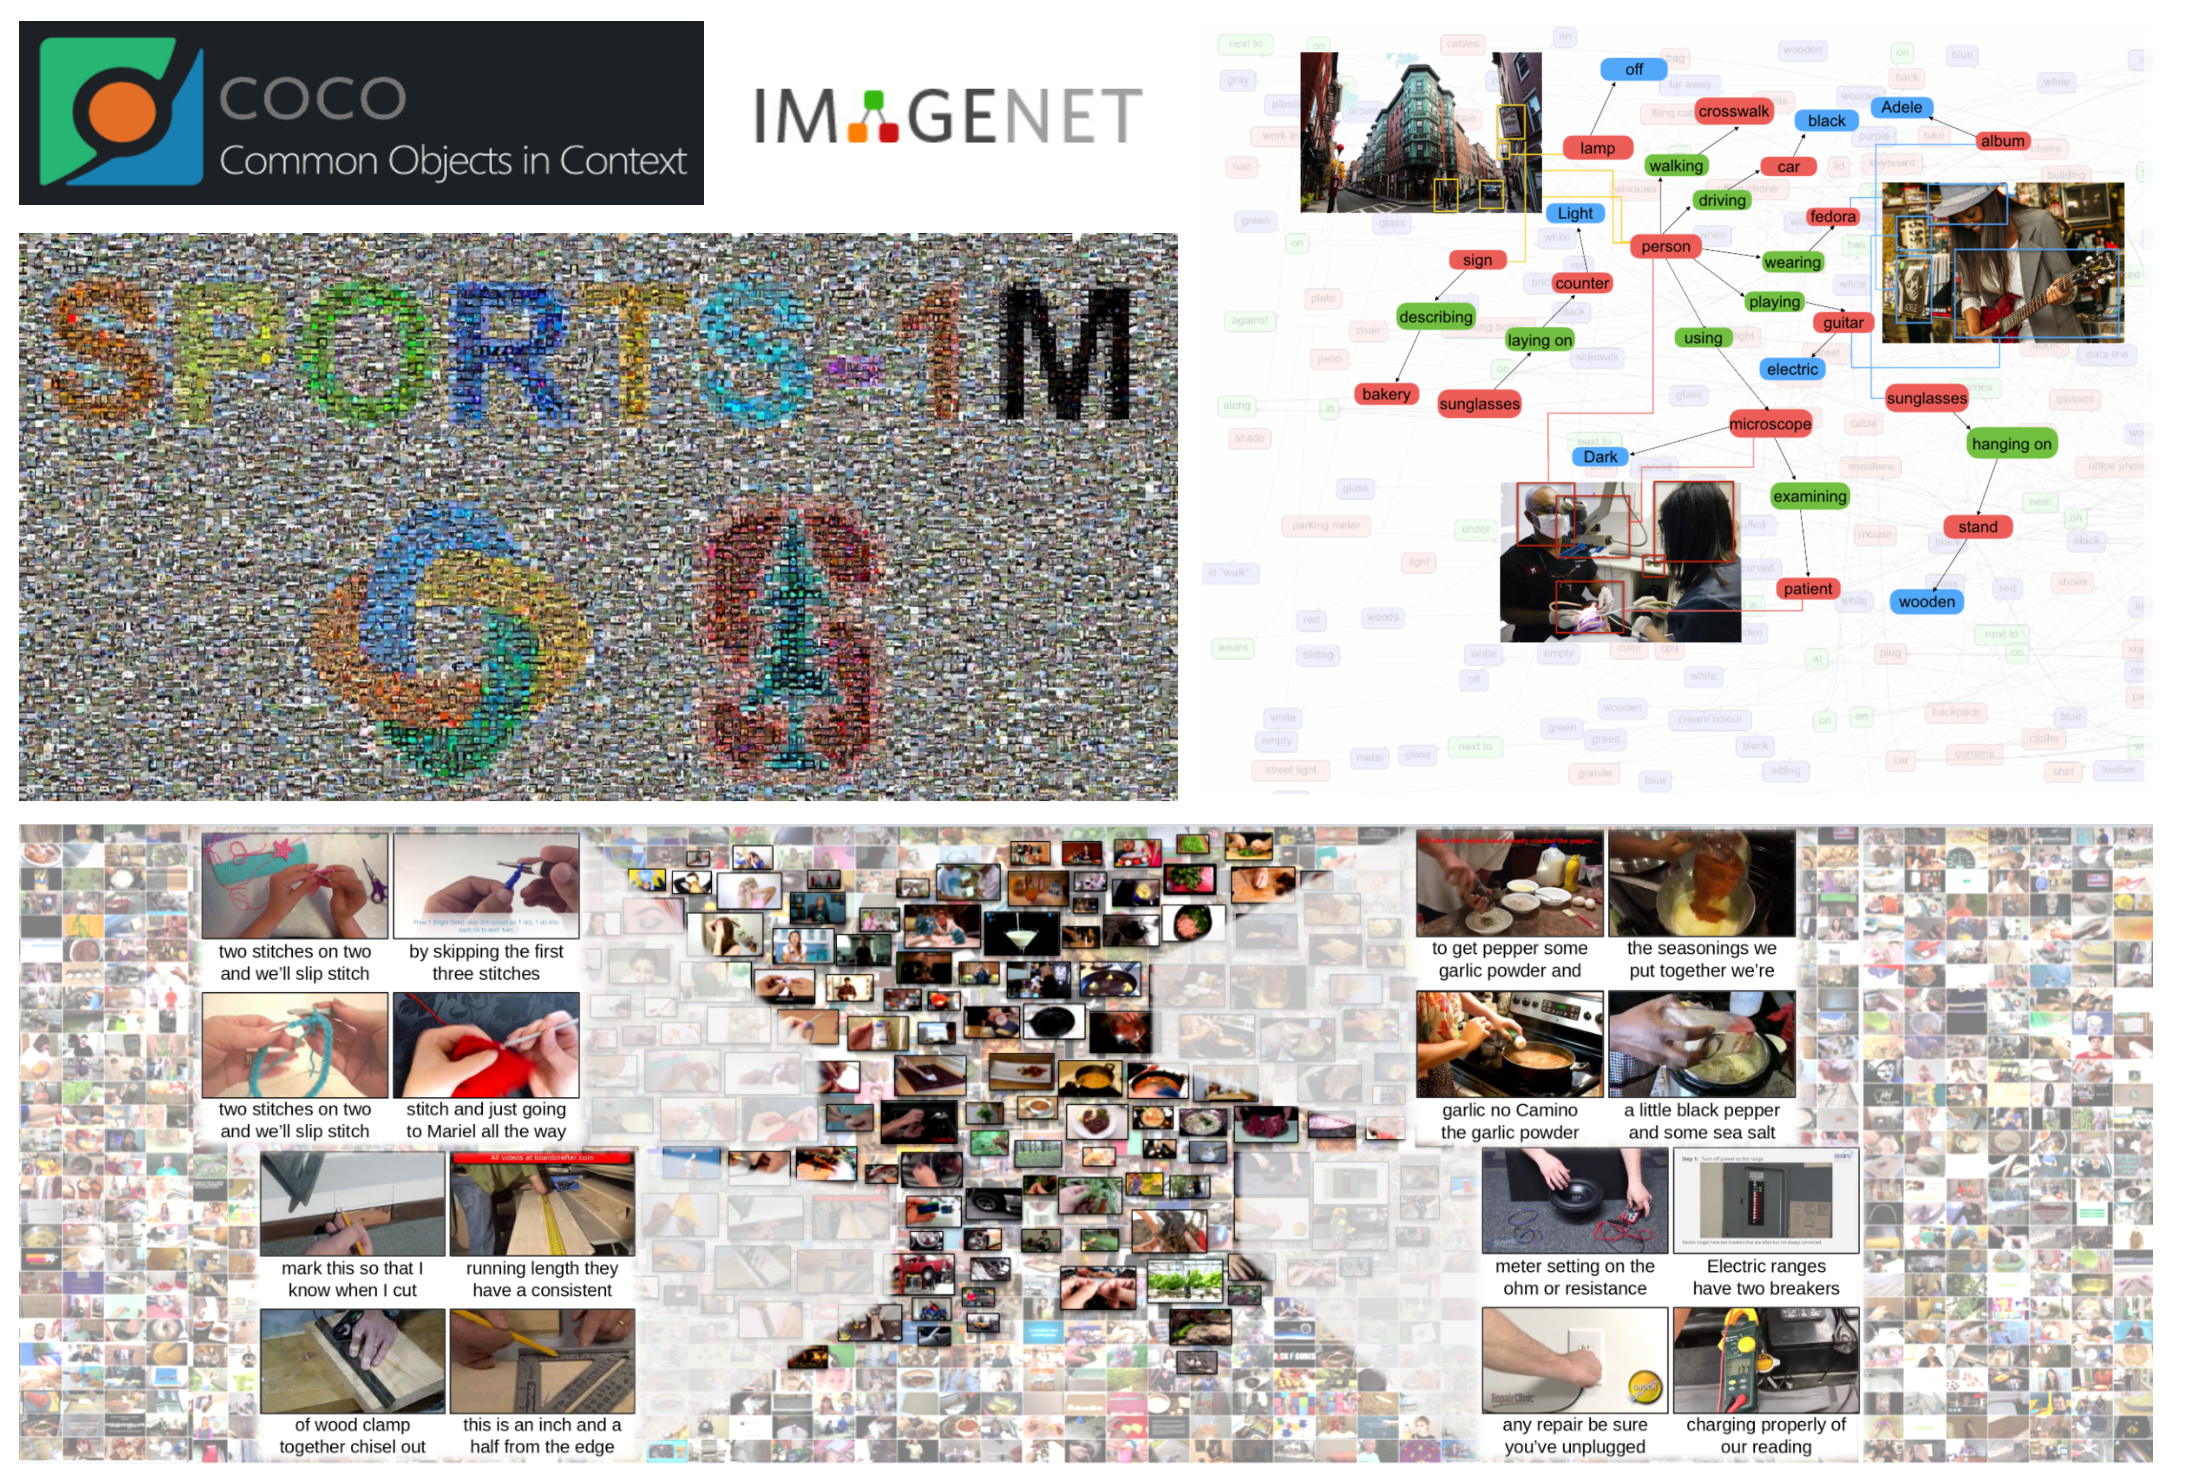
\includegraphics[width=0.95\linewidth]{chapter1/res/datasets_examples.pdf}
    \caption{众多大规模图像和视频数据集推动计算机视觉技术的发展}
    \label{ch1:fig:datasets_examples}
\end{figure}

对于复杂视觉场景的感知和理解,具体来说,主要包含四个不同的层次:1)对场景内单个物体进行识别(\textbf{物体级别识别});2)对场景内所有物体以及物体之间的视觉关系进行识别(\textbf{场景级别识别});3)对整个视觉场景的内容进行理解(\textbf{场景级别理解});4)在场景级别理解的基础上进行知识推理(\textbf{场景级别推理})。本文将针对这四个不同层次的视觉场景感知和理解,逐步地对复杂视觉场景中视觉内容的识别、检测和推理进行研究。如图~\ref{ch1:fig:scene_understanding}所示,本文的关键技术线路主要包含:(零样本)物体分类、场景图生成、视觉描述生成、视觉检索和视觉问答等具体研究任务:

\begin{figure}[t]
    \centering
        \includegraphics[width=0.95\linewidth]{chapter1/res/scene_understanding.pdf}
    \centering
    \caption{复杂视觉场景中视觉内容的识别、检测和推理的关键技术路线}
    \label{ch1:fig:scene_understanding}
\end{figure}

1)\textbf{物体级别识别}:视觉场景感知和理解的首要步骤就是对场景内包含的物体进行个体层次的识别。作为计算机视觉领域中一个最基本的问题,个体层次的物体识别结果将直接影响后续对整个视觉场景进行场景层次的识别、理解和推理。根据识别的粒度,物体级别识别通常包含物体分类、目标检测、实例分割等多种具体的视觉任务。其中物体分类任务~\cite{russakovsky2015imagenet,krizhevsky2012imagenet,simonyan2015very,szegedy2015going,he2016deep,xie2017aggregated,hu2018squeeze}只是对物体进行多类别分类,而目标检测任务~\cite{ren2015faster,liu2016ssd,redmon2016you}和实例分割任务~\cite{he2017mask}需要在物体分类的基础上,同时对物体的大致边框位置或精确像素位置进行定位。随着卷积神经网络的发展,在理想实验条件下,当每个类别的训练样本足够充足时,物体识别已经可以达到较高的准确率。然而,在日常生活中,所有类别的样本数量常常呈现“长尾分布”(long-tail distribution),即大量的类别往往缺乏足够的训练样本。例如,在大规模图像分类数据集ImageNet中,除最常见的1,000类图像以外,在剩余的21,814个类别中,有296个类别只有一张训练样本图像~\cite{russakovsky2015imagenet}。为了提升物体识别模型的通用性和鲁棒性,更加接近实际应用场景的少样本学习(Few-Shot Learning, FSL)~\cite{fei2006one}或零样本学习(Zero-Shot Learning, ZSL)~\cite{lampert2009learning}逐渐成为近年来的研究热点。然而,目前的零样本物体分类模型普遍存在语义丢失的问题(semantic loss),这将大大限制模型的迁移能力。本文将聚焦于零样本物体分类任务,研究如何缓解模型的语义丢失,提升模型的通用性和鲁棒性。

2)\textbf{场景级别识别}:视觉场景的组成元素除了大量的规则物体(object)外,还包括不规则物体(stuff),以及物体之间的视觉关系(visual relationship)等。因此,对整个视觉场景进行感知和理解的第二步就需要对场景中所有的不规则物体(如:全景分割~\cite{kirillov2019panoptic})和视觉关系(如:场景图生成~\cite{johnson2015image})进行识别。尤其对于复杂视觉场景来说,丰富的视觉关系通常“隐式地”包含场景内所有物体之间的内在联系。充分利用物体间的视觉关系不仅可以帮助提升单个物体的识别准确率,同时可以将非结构化的视觉场景内容转换成结构化的场景图(scene graph)。这些场景图可以看成视觉场景内容的一种抽象知识表达,能够辅助更高语义层级的场景级别的理解和推理。然而,目前的场景图生成模型主要都集中于研究如何更加有效地编码物体间的内在联系,并使用所有物体和视觉关系分类的交叉熵之和作为模型的优化目标。这个优化目标忽略了不同物体对整体场景图质量的贡献差异,大大降低了训练梯度的优化效率。本文将聚焦于图像场景图生成任务,研究如何设计更加合理的优化目标,提升场景图生成质量以及提供更加有效的训练梯度。

3)\textbf{场景级别理解}:在对整个视觉场景中所有的组成元素都完成识别之后,就可以开始对场景内容进行理解和推理。就场景级别理解而言,如何判断一个计算机模型对整个视觉场景的理解程度,通常缺乏统一的衡量方式和标准的评价指标。随着自然语言处理领域的发展,众多视觉和文本融合的多模态任务开始被当作场景级别理解的代理任务:如视觉描述生成~\cite{vinyals2015show}、视觉检索~\cite{gao2017tall}等。具体来说,视觉描述生成任务需要计算机模型生成自然描述语句,使得该语句刚好能够准确地概括整个视觉场景的内容。通过衡量最终描述语句的生成质量,来从侧面反映模型对视觉场景的理解程度。视觉检索任务需要计算机模型输出与给定查询内容完全一致的视觉场景。通过衡量最终的检索排序结果,来从侧面反映模型对视觉场景的理解程度。本文将聚焦图像描述生成(image captioning)和视频片段检索(Query-based Video Localization, QBVL)两个具体的场景级别理解任务,通过分析现有模型框架的优缺点,研究如何设计更加合理的网络结构,来提升计算机模型对视觉场景的理解。

4)\textbf{场景级别推理}:在对整个视觉场景内容进行充分理解之后,视觉场景理解的最终目标就是能够像人类一样进行知识推理。视觉问答(Visual Question Answering, VQA)~\cite{antol2015vqa}或视觉对话(visual dialog)~\cite{das2017visual}等场景推理任务,通常被看成是一种视觉图灵测试~\cite{malinowski2014towards,geman2015visual}。通过对视觉场景相关的内容进行提问,来判断模型的场景推理能力。由于测试问题的自由性和开放性,理论上一个理想的计算机模型需要同时具备物体识别、场景识别、空间推理、常识推理等多方面的能力。然而,现阶段的视觉问答模型往往都过于依赖数据集内部的文本偏置(language bias),并且忽略了两个重要特性:视觉可解释性和问题敏感性。本文将聚焦于视觉问答任务,研究如何减少文本偏置对视觉问答模型的影响,提升视觉问答模型的视觉可解释性和问题敏感性。


\section{研究内容}

本文主要研究如何对复杂视觉场景进行不同层次的感知和理解,结合现有的研究技术,提出更加优化的学习算法和更加合理的网络结构设计,具体可以归纳为图~\ref{ch1:fig:technique_summary}中所示方法。本文基于深度学习的方法对复杂视觉场景感知和理解中上述的关键技术进行研究,具体包括以下内容:

\begin{figure}[t]
    \centering
        \includegraphics[width=0.95\linewidth]{chapter1/res/technique_summary.pdf}
    \centering
    \caption{复杂场景识别、检测和推理的关键技术研究方法}
    \label{ch1:fig:technique_summary}
\end{figure}

\subsection{基于属性保持对抗网络的零样本物体分类}
复杂视觉场景的感知和理解,其首要步骤就是对视觉场景内的物体进行个体层次的识别。其中本文涉及到的关键技术为零样本物体分类,也称零样本学习。

目前主流的零样本物体分类模型都是基于嵌入映射的框架,这类方法主要是先在训练集上学习一个图像视觉特征与类别属性特征之间的映射函数,然后直接将学习到的映射函数迁移到测试集中。由于训练集和测试集之间的类别存在差异,这些映射函数在测试集中不可避免地存在语义丢失的问题。针对这一普遍问题,本文提出一种全新的零样本学习网络:基于属性保持的对抗网络。该网络通过引入两个独立的映射网络分支,将图像分类和图像重建两个原本相互冲突的任务分离出来。然后利用对抗网络学习让重建网络的特征向量的部分属性能够迁移到分类网络的特征向量中,从而使得分类网络的特征向量能够保持尽可能多的属性,缓解语义丢失的问题。本文提出的零样本学习网络不仅可以逼真地重建回原始图像,同时可以在多个数据集上大幅度地提升零样本分类的准确率。

\subsection{基于反事实多智能体学习的图像场景图生成}
在复杂视觉场景的识别中,除了需要对场景内所有的单个物体进行识别,还需要检测物体间的视觉关系。图像场景图生成任务主要研究如何充分地利用视觉场景内各种视觉元素间的内在联系,实现场景级别的识别。

现有的图像场景图生成方法几乎都是将场景内所有的物体和视觉关系分类的交叉熵之和作为模型的优化目标。这个优化目标的本质是认为每个物体分类的损失是相互独立的,即它忽略了不同物体对整体场景图生成质量的不同贡献,容易使模型陷入局部最优解。本文提出了一种全新的训练框架,将图像场景图生成任务转换成一个多智能体协同决策问题,并且直接使用最终的场景图生成质量评价指标(即:Recall@K)作为模型的优化目标。具体来说,我们将图像中的每个物体看成一个单独的智能体,每个智能体的动作空间是所有可能的物体类别。同时,本文提出了一个全新的反事实基准模型,通过固定其他智能体预测的类别,而反事实地“更改”目标智能体的预测类别,来推测目标智能体预测类别对整体场景图生成质量的局部贡献。本文提出的反事实多智能体学习框架可以通过提升物体类别的预测准确率,显著提升整个场景图的生成质量。


\subsection{基于多层空间和通道注意力网络的图像描述生成}

图像描述生成是一种典型的视觉场景理解任务。该任务要求模型在对整个视觉场景进行充分的理解之后,生成自然语句来准确地描述场景内容。

现有的图像描述生成模型都是基于编码器-解码器(encoder-decoder)框架:即利用编码网络(如:卷积神经网络)将图像编码成视觉特征向量,然后利用解码网络(如:递归神经网络)将编码的视觉特征向量解码成自然语句。早期的图像描述生成模型都是只将图像编码成一个固定的视觉特征向量,这大大限制了视觉特征向量的表达能力。之后,部分模型开始引入空间注意力机制,通过在每个单词生成的时刻对不同空间区域的视觉特征赋予不同的权重,进行加权得到不同的视觉特征向量。然而,卷积神经网络的特征图(feature map)除了空间维度外,还包含通道和层级两个维度。在不同的通道和层级下,卷积神经网络的特征图所编码的视觉信息也往往不同。本文提出一种全新的多层空间和通道注意力网络,不仅可以充分地挖掘特征图的三个维度之间的联系,提升了编码网络的表达能力,同时,还可以帮助人们理解在图像描述生成过程中卷积神经网络的特征图的变化过程。


\subsection{基于密集型自底向上网络的视频片段检索}

视频片段检索任务也是一种具有广泛应用价值的视觉场景理解任务。给定一个查询内容(query),视频片段检索任务需要模型在视频中定位出与查询内容相匹配的视频片段。

对于视频片段检索任务,目前的方法都属于自顶向下框架或稀疏型自底向上框架。本文首先分析了现有的视频片段检索的主流框架的优缺点,然后针对稀疏型自底向上模型的设计缺陷,我们提出了一种全新的密集型自底向上框架。具体来说,我们将边界预测问题分解成相关性预测和边界回归两个子问题,大大降低了视频动作边界定位问题的难度。同时,我们提出一个基于图卷积的特征金字塔层,来增强骨干网络编码能力。该框架显著地提升了自底向上模型的检索准确率。对于多种不同的查询形式(如:自然语句或视频片段等),本文提出的密集型自底向上模型都达到了当时最好的性能。


\subsection{基于反事实样本生成的视觉问答}

视觉场景理解的最终目标就是能够在对整个场景内容完成理解之后进行知识推理。视觉问答是最经典的一种视觉推理任务,给定一个与视觉场景内容相关的问题,模型需要在经过一系列逻辑推理之后给出问题的答案。

尽管近年来涌现了大量的视觉问答模型,但是这些方法几乎都忽略了一个理想视觉问答模型应当具备的两个重要能力:视觉可解释性和文本敏感性。为了提升视觉问答模型的这两个能力,本文提出了一种全新的反事实样本生成机制。通过人为地遮盖图像中的重要区域或问题中的重要单词,同时更改标准答案,来合成大量的反事实训练样本。通过使用原始训练样本和新合成的反事实训练样本一起对视觉问答模型进行训练,迫使模型关注反事实训练样本中被遮盖的重要内容,即让模型在决策时能够更加关注“重要的”视觉区域和单词,提升模型的视觉可解释性和问题敏感性。本文提出的反事实样本生成机制可以无缝地运用到任意的视觉问答模型中,提升模型的鲁棒性和准确率。


\section{本文组织结构}
本文通过对复杂视觉场景理解中视觉内容的识别、检测和推理中的一系列典型问题,提出了多个更加优化的学习算法和更加合理的网络结构。本论文总共分为八章,之后的章节内容安排如下:

\begin{asparaitem}

\item 第二章介绍了与复杂视觉场景理解相关的关键技术研究,就零样本物体分类、图像场景图生成、图像描述生成、视频片段检索和视觉问答等几方面的相关工作和本文的关系进行综述。

\item 第三章介绍了基于属性保持对抗网络的零样本物体分类方法。本章首次提出图像分类与图像重建本质上是相互冲突的两个子任务。算法通过引入两个独立的映射网络分支,将图像分类和图像重建两个任务分离出来。然后利用对抗网络学习让重建网络的特征向量的部分属性能够迁移到分类网络的特征向量中,从而使得分类网络的特征向量保持尽可能多的属性,缓解语义丢失的问题。此项工作发表在国际顶级计算机视觉会议CVPR上。

\item 第四章介绍了基于反事实多智能体学习的图像场景图生成方法。本章首次将
图像场景图生成问题转化为一个多智能体协同决策问题,并且直接使用整体的场景图生成质量作为优化目标,避免模型陷入局部最优解。同时,本章提出一个全新的反事实基准模型,有效地对不同物体的预测类别赋予不同的优化梯度,显著提升了物体类别的预测准确率和整体场景图的生成质量。此项工作发表在国际顶级计算机视觉会议ICCV上。

\item 第五章介绍了基于多层空间和通道注意力网络的图像描述生成方法。本章首次提出通道注意力机制,并认为通道注意力机制本质上也属于一种特殊的语义注意力机制。同时,本章提出一种全新的多层空间和通道注意力网络,不仅充分挖掘了卷积神经网络的特征图的三个维度(空间、通道和层级)之间的联系,提升了编码网络的表达能力。同时,还可以帮助人们理解在图像描述生成过程中卷积神经网络的特征图的变化过程。此项工作发表在国际顶级计算机视觉会议CVPR上。

\item 第六章介绍了基于密集型自底向上网络的视频片段检索方法。本章首次提出了一种密集型自底向上网络框架。通过将边界预测问题分解成相关性预测和边界回归两个子问题,大大降低了模型对视频动作边界定位的难度。同时,本章提出了一个基于图卷积的特征金字塔层,来增强骨干网络编码能力。该框架显著地提升了视频片段检索的准确率。此项工作发表在国际顶级人工智能会议AAAI上。

\item 第七章介绍了基于反事实样本生成的视觉问答方法。本章首次提出了一种通用的反事实训练样本生成方法,提升视觉问答模型的视觉可解释性和文本敏感性。本文提出的反事实样本生成机制可以无缝地运用到任意的视觉问答模型中,提升模型的准确率和鲁棒性。此项工作发表在国际顶级计算机视觉会议CVPR上。

\item 第八章对全文所有介绍的工作进行了总结,并提出了在今后进一步对复杂场景理解的识别、检测和推理的研究内容以及研究展望。

\end{asparaitem}

\section{本章小结}
本章对复杂视觉场景的识别、检测和推理问题进行了叙述,分别介绍了研究背景、本文的主要研究内容以及全文的组织结构。



\chapter{相关研究综述}

本章将就零样本物体分类、图像场景图生成、图像描述语句生成、视频片段检索和图像视觉问答几方面的相关工作和本文的关系进行综述。

本文提出的算法和其相关工作的具体细节和对比将在之后各章节中展示。


\section{零样本物体分类}

\subsection{零样本学习}
零样本物体分类,或零样本学习,通过利用所有类别(即:已见类别和未见类别)在属性空间的关联性~\cite{farhadi2009describing,lampert2009learning,romera2015embarrassingly,norouzi2014zero,demirel2017attributes2classname,jiang2017learning},将类别属性看成是一个共同语义空间的中间特征,实现知识从已见类别到未见类别之间的迁移。早期的零样本学习模型通常为二阶段模型~\cite{lampert2013attribute,norouzi2014zero,al2016recovering,jayaraman2014zero,kankuekul2012online}。在第一阶段,模型预测出图像包含的属性特征;在第二阶段,模型根据预测的属性特征推测出物体的类别。

为了扩大零样本迁移能力,目前的大多数方法都是基于嵌入映射的~\cite{palatucci2009zero,frome2013devise,akata2015label,akata2015evaluation,romera2015embarrassingly,xian2016latent,socher2013zero,kodirov2017semantic,li2017zero}:通过学习图像的视觉特征向量和类别的语义嵌入向量之间的映射函数,实现零样本分类。最早的基于嵌入映射的模型是SOC~\cite{palatucci2009zero}。SOC通过将图像特征从视觉空间直接映射到语义空间,然后在语义空间与类别属性的嵌入向量进行相似度对比。之后,ALE~\cite{akata2015label}和DeViSE~\cite{frome2013devise}开始提出使用排序损失函数(ranking loss)作为优化目标。除了将视觉图像特征线性地映射到语义空间,LatEm~\cite{xian2016latent}开始使用非线性的映射函数。CMT~\cite{socher2013zero}使用两层神经网络的将视觉图像特征映射到语义空间中。为了进一步提升图像视觉特征的表达能力,Ba等人~\cite{lei2015predicting}提出要让图像编码网络和映射网络一起端到端训练。同样地,Zhang等人~\cite{zhang2017learning}认为图像的视觉特征空间比类别的语义空间具有更强的区分能力,通过将类别属性的嵌入向量映射到视觉空间中,然后通过端到端训练可以进一步提升零样本分类效果。与此同时,部分模型开始提出将图像的视觉特征和类别的语义特征都映射到其他的共同空间。例如:SSE~\cite{zhang2015zero}直接将已见类别的线性组合作为共同空间。JLSE~\cite{zhang2016zero}分别讲图像的视觉特征和类别的语义特征分别映射到两个单独的子空间,然后计算两个子空间的相似度。

类别在语义空间中的嵌入向量主要来自于属性标注,但是由于属性信息需要大量的人工标注。一些工作开始研究使用其他的辅助信息来减少模型需要的属性标注。如SJE~\cite{akata2015evaluation}使用了四种嵌入向量:属性、word2vec~\cite{mikolov2013distributed}、GloVe~\cite{pennington2014glove}和wordnet~\cite{miller1995wordnet}。另外,嵌入向量不仅可以来自于单词,也可以来自于图像的描述语句~\cite{reed2016learning,lei2015predicting,elhoseiny2013write}。


\subsection{通用型零样本学习}
在之前的零样本物体分类(即:传统型零样本学习)中,测试阶段的所有图像都只来自于未见类别,即模型预测类别的选择空间只限于未见类别。这种实验设定大大降低了零样本学习的难度以及在实际场景中的运用价值。随着通用型零样本学习~\cite{scheirer2012toward}的提出,模型在测试阶段需要对所有类别(已见类别和未见类别)的图像进行类别预测。Bendale等人~\cite{bendale2016towards}首次将通用型零样本分类问题看成异常检测问题,利用一个网络先判断图像是否来自未见类别。对于通用型零样本学习,由于训练时使用了大量的已见类别图像而没有使用任何未见类别图像,模型往往倾向于将图像分类成已见类别。为了更好的评估通用型零样本分类,许多工作提出了不同的评价指标~\cite{chao2016empirical,xian2018zero}来权衡已见类别和未见类别。

在本文,我们也重点研究通用型零样本物体分类。据我们了解,本文提出的属性保持的对抗网络学习模型(SP-AEN)是零样本分类算法中,第一个可以用语义空间的嵌入向量来重建原始图像。

\subsection{零样本学习中的域偏移问题}
属性损失问题,也常常被称为域偏移问题(domain shift)~\cite{fu2015transductive,saenko2010adapting},是零样本学习、少样本学习~\cite{hariharan2017low}或领域自适应~\cite{motiian2017unified,panareda2017open}
等任务中一个非常普遍存在的问题。只要训练集数据和测试集数据的分布不同,就存在域偏移。目前的研究工作都发现重建原始信号可以缓解域偏移问题~\cite{kim2017learning}。在零样本分类领域,Kodirov等人~\cite{kodirov2017semantic}通过同时进行图像分类和语义属性重建来缓解属性丢失问题。在本文,我们通过实验发现利用同一个网络同时进行重建和分类这两个相互冲突的任务对于保持语义特征并不是很有效。与此同时,另一种缓解语义损失的办法是增加一个单独的属性分类器~\cite{morgado2017semantically},但是这个方法需要额外的属性标注信息。

\subsection{零样本学习和对抗生成网络}
对抗生成网络~\cite{goodfellow2014generative}主要是训练一个生成器,使得生成器生成的样本和真实数据非常“相似”,可以“骗过”判别器。理论上,这种对抗的训练过程可以让生成器生成的样本分布和真实的样本分布完全相同。对于零样本分类问题,一些模型开始借助于对抗生成网络来生成更多的训练样本,从而将零样本分类问题转化为普通的分类问题~\cite{mishra2018generative,xian2018feature,xian2019f}。尽管这类方法目前已经取得很好的实验性能,但是它们违背了零样本分类问题的一个基本假设:训练阶段中测试集的类别信息是无法知道的。相反,本文提出的零样本分类模型SP-AEN只是将对抗网络中的对抗思想运用到特征层面上~\cite{odena2017conditional,tzeng2017adversarial,makhzani2015adversarial,shrivastava2017learning},使得分类特征向量的分布向重建特征向量的分布靠近,进而让分类特征向量尽可能地保持更多的属性特征,提升模型的迁移能力。



\section{图像场景图生成}

\subsection{场景图生成}
随着视觉关系检测任务~\cite{lu2016visual}和大规模图像场景图数据集~\cite{krishna2017visual}的出现,图像场景图生成任务逐渐成为一个新的研究热点。目前,绝大多数的场景图生成模型都是将场景图生成任务分为两个步骤:1)利用预训练好的目标检测器~\cite{lu2016visual,zhuang2017towards,zhang2017visual,dai2017detecting,yang2018shuffle,yu2017visual}或在图像场景图生成数据重新微调的目标检测器~\cite{li2017vip,xu2017scene,yin2018zoom,zellers2018neural,zhang2017relationship,zhang2019large}对图像进行目标检测。2)对于所有检测的物体的类别以及两两物体间的视觉关系类别进行预测。在早期阶段,许多模型都将物体类别预测和视觉关系类别预测拆分成两个独立的任务~\cite{lu2016visual,zhang2017visual,zhuang2017towards,zhu2018deep,zhang2017relationship}。这样的拆分忽略了场景内所有所有物体间的内在联系。为了充分利用场景内所有物体间的诱导偏置(inductive bias),一些场景图生成模型开始利用信息传递机制(message passing)~\cite{xu2017scene,dai2017detecting,li2017scene,li2018factorizable,yin2018zoom,jae2018tensorize,yang2018graph,tang2019learning,gu2019scene,qi2019attentive,wang2019exploring}。例如:Xu等人~\cite{xu2017scene}将物体和视觉关系分别看成两个独立的递归神经网络的节点,在递归神经网络的每个迭代过程中两个节点互相传递信息,每个物体节点和视觉关系节点通过接收传递的信息来更新自身节点的内部特征表达,从而充分利用图像的上下文全局信息。Li等人~\cite{li2017scene}通过引入图像密集描述生成任务,构建三层语义节点(物体、视觉关系以及密集描述框),然后同样利用信息传递机制更新三种节点的特征表达。Yang等人~\cite{yang2018graph}利用图卷积,对每个物体周围的特征进行加权。之后,Zellers等人~\cite{zellers2018neural}发现目前数据集中标注的视觉关系包含大量的文本偏置,即利用物体类别和视觉关系类别之间的统计频率就可以得到较高的视觉关系预测准确率。目前,最新的模型都将训练集图像中视觉关系的统计频率作为场景图中视觉关系的先验知识。

然后,之前所有的方法都关注于如何编码周围的信息来增强物体特征,所有的这些模型都使用物体和视觉关系分类的交叉熵作为模型最终的优化目标。这个优化目标将图像中所有的物体的重要性看成完全相同,即忽略了不同物体间的重要性,容易让模型陷入局部最优解。本文,首次将最终的场景图生成质量作为整体优化目标,并首次将场景图生成任务看成多智能体协同合作的决策问题。

\subsection{多智能体策略梯度}

策略梯度即是一种强化学习的优化策略,同样也是一种对不可导优化目标进行优化的方法。在视觉场景理解任务中,策略梯度已经广泛应用在多种任务中,如:图像描述生成~\cite{ranzato2016sequence,ren2017deep,liu2017improved,rennie2017self,zhang2017actor,liu2018context},图像视觉问答~\cite{hu2017learning,johnson2017inferring},图文匹配~\cite{chen2017query,yu2017joint},视觉对话~\cite{das2017learning},和目标检测~\cite{caicedo2015active,mathe2016reinforcement,jie2016tree}。目前,所有的场景图生成模型中,只有Liang等人~\cite{liang2017deep}将图像场景图生成任务看成一个单智能体的序列决策过程。它首先根据文本的先验信息构建一个有向的语义图,在决策过程的每一个步骤中,选取新的物体和视觉关系,逐渐构建视觉场景图。相反,本文将图像场景图生成任务看成一个多智能体协同决策过程。通过构建成多智能体协同决策过程,我们可以直接使用整体场景图生成质量作为优化目标。另外,与目前许多现有的多智能体协同工作不同~\cite{foerster2016learning,omidshafiei2017deep},本文的模型中,单个图像中智能体的数量(64个检测物体)与动作空间范围(151个物体类别)都非常大。


\section{图像描述生成}

\subsection{编码-解码框架}

图像描述生成任务(Image Captioning)通常被认为是一种多模态的“翻译”任务,即模型将视觉图像“翻译”成自然语言描述。由于端到端编码-解码框架在机器翻译任务(Neural Machine Translation, NMT)~\cite{sutskever2014sequence}的成功,许多的图像描述生成模型也开始借鉴使用编码-解码框架。最早的基于编码-解码框架的图像描述生成模型是NIC~\cite{vinyals2015show}。NIC用一个卷积神经网络将原始输入图像编码成一个固定的视觉特征向量,然后将该视觉特征向量作为一个递归神经网络的初始时刻的输入,利用递归神经网络逐步将视觉特征向量解码成描述语句。类似地,Karpathy等人~\cite{karpathy2015deep}将编码的视觉特征向量作为递归神经网络隐含状态的初始化,通过引入一个额外的“START”字符触发递归神经网络对视觉特征进行解码。

由于在大规模图像分类数据集ImageNet预训练的卷积神经网络(如:VGG~\cite{simonyan2015very}、GoogLeNet~\cite{szegedy2015going}、ResNet~\cite{he2016deep}等)通常可以提取较好的图像视觉特征,之后的许多基于编码-解码框架的改进工作主要集中于完善解码过程。例如,Donahue等人~\cite{donahue2015long}和Mao等人~\cite{mao2015deep}提出在递归神经网络迭代的每个时刻都输入视觉特征向量,避免生成句子过长时图像特征的影响逐渐减弱。Wang等人~\cite{wang2016image}提出使用双边递归神经网络作为解码器,避免单向递归神经网络LSTM~\cite{hochreiter1997long}只考虑之前时刻的单词信息。

\subsection{注意力机制}

在解码器生成语句的过程中,可以通过引入注意力机制~\cite{bahdanau2014neural}使得模型在预测每个单词的时候动态地调整视觉特征向量,增强编码器的表达能力。

\textbf{空间注意力机制}:Xu等人~\cite{xu2015show}首次将注意力机制应用于图像描述生成任务中。具体来说,Xu等人在卷积神经网络的最后一层特征图中引入空间注意力机制,让模型在每个时刻动态地关注不同的空间区域,合成新的视觉特征。类似地,Zhu等人将同样的空间注意力机制也运用到图像视觉问答任务~\cite{zhu2016visual7w}。除了在最后一层特征图只使用一次空间注意力加权,Yang等人~\cite{yang2016stacked}和Xu等人~\cite{xu2016ask}提出通过叠加使用多次空间注意力加权来提升模型性能。相比于之前的模型只在卷积神经网络的特征图中使用空间注意力加权,Anderson等人~\cite{anderson2018bottom}和Li等人~\cite{li2016visual}提出先对图像进行目标检测,然后对物体级别特征使用空间注意力机制可以进一步提升模型性能。

\textbf{语义注意力机制}:除了对图像的不同视觉区域加权,一些模型开始引入图像包含的属性,作为额外的语义信息,来引导语句的生成~\cite{wu2016what,you2016image,pan2017video,yao2017boosting}。其中,You等人~\cite{you2016image}提出语义注意力机制,通过对不同的属性赋予不同的权重,在生成单词的过程中不断关注相关的属性。Yao等人~\cite{yao2017boosting}不仅引入属性来提升图像的描述语句生成,同时研究如何设计网络结构使得模型在生成描述语句过程中能够更好的利用属性信息。Jia等人~\cite{jia2015guiding}通过将图像和当前生成语句的相关性看成一个全局的语义信息,来引导语句生成。但是,这些模型需要额外地提取语义信息,如属性等。在本文提出的多层空间和通道注意力网络中,每个卷积核可以看成是多个语义检测器~\cite{zeiler2014visualizing}。因此,通道注意力机制可以看成是一种特定的语义注意力机制。


\textbf{自注意力机制}:自注意力机制~\cite{vaswani2017attention}先将特征集合(如图像区域特征)通过不同的映射矩阵分别映射为查询特征矩阵(query)、键特征矩阵(key)和值特征矩阵(value)。通过查询特征矩阵和键特征矩阵计算相似度得到注意力权重矩阵,然后对值特征矩阵进行加权,得到加权后的特征向量。基于自注意力机制的图像描述生成主要是利用Transformer结构~\cite{vaswani2017attention}:用编码网络对图像进行编码,解码网络对编码特征进行解码。其中编码网络和解码网络中都包含大量的自注意力机制模块。Herdade等人~\cite{herdade2019image}首次基于Transformer结构,并且将图像中物体间的几何位置作为重要的语义信息,帮助生成描述语句。与此同时,Li等人~\cite{li2019entangled}通过引入外部的语义标签来增强图像描述的内容。Huang等人~\cite{huang2019attention}引入额外的注意力机制对加权后的特征进行再一次加权。不同于之前的模型都只基于原始的Transformer结构,Cornia等人~\cite{cornia2020m}通过将编码网络中所有层级的特征都作为每层解码网络的输入,对Transformer结果进行改进,进一步提升描述语句生成质量。



\section{视频片段检索}

\subsection{视频片段检索}

\textbf{基于语句查询的视频片段检索}:
基于语句查询的视频片段检索,是一个典型的多模态问题。目前,主流的方法都是基于自顶向下的框架,这些方法主要关注如何设计更强的多模态融合模型,如基于视频的查询注意力机制~\cite{liu2018attentive}、基于查询的视频注意力机制~\cite{liu2018cross}、查询-视频的协同注意力机制~\cite{chen2018temporally,chen2019localizing,yuan2019find}。据我们了解,绝大多数的模型都是自顶向下或自底向上框架,只有两个例外:RWM~\cite{he2019read}和SM-RL~\cite{wang2019language}。这两个方法都是将视频片段检索问题转换成时序决策问题,然后利用梯度策略进行优化,其中的动作空间为时序窗口的变化或帧的跳变。

\textbf{基于视频查询的视频片段检索}:
基于视频查询的视频片段检索的主要困难来自于查询视频和参考视频之间巨大的场景差异,包括背景、物体、视角等不同。目前最好的视频查询的视频片段检索是CGBM~\cite{feng2018video},它也是基于稀疏型自底向上模型。


\subsection{自顶向下与自底向上}
自顶向下和自底向上方法,是计算机视觉研究领域解决问题的两种重要的思考哲学。与本文提出的自底向上框架最为接近的概念是:

\textbf{目标检测}:随着目标检测器Faster R-CNN~\cite{ren2015faster}的出现,目前绝大多数的目标检测算法都是基于自顶向下的框架,即在每个位置上预先定义大量的锚框,然后对每个锚框进行类别分类和坐标位置回归。这类自顶向下的模型拥有和自顶向下的视频片段查询方法一致的缺点。随着第一个性能相当的自底向上目标检测器的出现:CornerNet~\cite{law2018cornernet},自底向上的目标检测模型开始逐渐受到关注,近期也推出了大量的自底向上的目标检测器~\cite{zhou2019bottom,zhou2019objects,duan2019centernet,tian2019fcos}。

\textbf{注意力机制}:自底向上注意力机制在许多的视觉-文本等多模态任务中发挥重要的作用,例如:图像描述生成~\cite{xu2015show,chen2017sca},视觉问答~\cite{xu2016ask,ye2017video}等。最近,Anderson等人~\cite{anderson2018bottom}提出融合自底向上和自顶向下的注意力机制,进一步提升了多个任务的模型性能。因此,如何更好的融合或权衡自顶向下与自底向上两种方法,将是未来的一个重要的研究方向。


\section{图像视觉问答}

\subsection{视觉问答模型}

典型的图像视觉问答模型通常包含一个图像编码模块、一个文本编码模块、一个融合模块和一个分类器。图像编码模块和文本编码模块分别对图像和问句进行编码,然后利用融合模块将两个模态的编码向量进行融合,最后分类器直接基于融合后的多模态特征进行答案预测~\cite{zhou2015simple,antol2015vqa,kim2016multimodal}。由于每个不同的问句往往涉及到图像的不同区域,之前的模型利用图像编码模块对图像提取统一的全局特征容易忽略一些重要的细节。为了避免上述问题,一些视觉问答模型开始引入注意力机制来动态提取视觉特征。Chen等人~\cite{chen2016abc}将问句的特征向量映射成一个卷积核,然后对图像的视觉特征卷积层进行卷积。Yang等人~\cite{yang2016stacked}通过迭代多个空间注意力机制,逐渐优化空间注意力的权重。Fukui等人~\cite{fukui2016multimodal}、Kim等人~\cite{kim2017hadamard,kim2018bilinear}、Yu等人~\cite{yu2017multi,yu2018beyond}、Ben等人~\cite{ben2017mutan,ben2019block}分别提出了不同的多模态双线性融合方式来融合文本特征(即问句)和不同图像区域特征。Anderson等人~\cite{anderson2018bottom}提出自底向上和自顶向下注意力机制,通过对物体框进行注意力机制,而不是直接对图像的不同特征层区域使用注意力机制。

除了对图像进行充分的理解外,视觉问答同时还需要对问句进行理解。因此,对问句使用注意力机制同样可以提取更加重要的文本信息。Lu等人~\cite{lu2017hierarchical}提出协同注意力机制(co-attention mechanism)同时对图像和问句进行注意力加权。Yu等人~\cite{yu2018beyond}通过在问句中使用自注意力机制对协同注意力机制进行简化。早期的协同注意力机制只是在单个模态下分别进行注意力加权,之后,Nguyen等人~\cite{nguyen2018improved}、Kim等人~\cite{kim2018bilinear}、Gao等人~\cite{gao2019dynamic}、Yu等人~\cite{yu2019deep}分别提出“密集型”协同注意力机制,充分计算每一个单词特征和每一个图像视觉特征之间的交互,进一步提升视觉问答性能。


\subsection{视觉问答模型的文本偏置}

尽管所有的视觉问答模型都在融合了多模态的特征之后进行答案预测,但是大量的研究工作表明~\cite{jabri2016revisiting,agrawal2016analyzing,zhang2016yin,goyal2017making},目前的视觉问答模型预测答案时往往都依赖文本偏置。为了减少文本偏置对视觉问答的影响,主要有两种解决方案:

\begin{asparaenum}

\item \textbf{收集更平衡的数据集}:减少文本偏置最简单的方法就是收集更加平衡的数据集。例如:Zhang等人~\cite{zhang2016yin}通过对抽象数据集中所有的判断题收集互补的场景图像,使得判断题的答案刚好完全相反。Goyal等人~\cite{goyal2017making}对真实图像数据集的所有类型的问题都收集互补的图像,使得标准答案与原始图像不同。虽然这些数据集在一定程度上可以缓解文本偏置的问题,但是由于训练集和测试集的问题答案分布基本一致,目前的模型仍然可以通过统计的偏置得到较高的准确率~\cite{agrawal2018don}。例如,在数据集VQA-CP中,当训练集和测试集的问题答案分布不同时,模型都会出现明显的性能下降。本文,我们同样是参考这个思路,来生成更多的互补样本。相反,本文提出的反事实样本生成机制(Counterfactual Samples Synthesizing, CSS)不需要任何额外的人工标注。

\item \textbf{设计更合理的去偏置模型}:另一种减少文本偏置的方法就是设计更合理的去偏置模型。到目前为止,效果最后的去偏置模型就是复合模型~\cite{ramakrishnan2018overcoming,grand2019adversarial,belinkov2019don,cadene2019rubi,clark2019don,mahabadi2019simple}:通过引入一个辅助网络来约束视觉问答网络的训练,其中的辅助网络只用文本(即问题语句)作为输入。在本文,我们提出的反事实样本生成机制可以无缝地应用于复合模型中,进一步减少文本偏置的影响。

\end{asparaenum}

\subsection{视觉问答模型的特性}

视觉可解释性和文本敏感性是一个理想的视觉问答模型必不可少的两个特性:
\begin{asparaenum}
\item \textbf{视觉可解释性}:为了提升视觉可解释性,早期的视觉问答模型~\cite{qiao2018exploring,liu2017attention,zhang2019interpretable}都直接使用人类关注的区域作为额外的监督信息。然而,由于强大的文本偏置,即使模块关注到正确的图像区域,后续的网络结构仍然会忽视这部分视觉信号~\cite{selvaraju2019taking}。因此,最近的一些视觉问答工作~\cite{selvaraju2019taking,wu2019self}开始使用工具Grad-CAM~\cite{selvaraju2017grad}来计算每个物体对正确答案的贡献,然后让不同物体的贡献度与人工标注的一致。但是,这类方法有两个明显的缺点:1)它们需要额外的人工标注,即每个物体的贡献度大小或者排序;2)目前这类方法都不是端到端训练的。

\item \textbf{文本敏感性}:如果一个视觉问答模型能够充分理解问题的含义,那么这个模型应该对问题的变化十分的敏感,即具备文本敏感性。据我们所知,目前只有一个工作讨论了视觉问答模型的文本敏感性~\cite{shah2019cycle}。具体来说,Shah等人~\cite{shah2019cycle}对于视觉问答和视觉问题生成两个对偶任务设计了一个循环一致的损失函数,然后通过引入随机噪声来生成不同的问题。然后,他们只考虑了对不同语句表达时的鲁棒性。相反,本文提出的反事实样本生成机制帮助模型能够感知重要单词的改变,提升文本敏感性。
\end{asparaenum}
目前的方法都只关注于视觉可解释性或着文本敏感性。相反,本文提出的反事实样本生成机制可以提升着两个特性。


\chapter{基于属性保持的零样本物体识别方法}

\section{引言}

\section{属性保持的对抗网络学习}

\section{实验设置与性能对比}

\section{本章小结}

\chapter{基于反事实多智能体学习的图像场景图生成方法}

图像场景图(scene graph)是将图像中每个物体当成一个节点,两两物体之间的视觉关系看成节点间的有向边,即视觉三元组“主语(物体)$\to$谓语(视觉关系)$\to$宾语(物体)”。图像场景图描绘了整个图像视觉场景中所有物体的类别、位置以及物体间的交互。为了生成准确的场景图,现有的场景图生成方法几乎都是通过“信息传递机制”(message passing),让每个物体和视觉关系都能充分地考虑和融合周围的视觉信息。例如,物体“人”和物体“自行车”之间一个最常见的视觉关系就是“骑”(即“人$\to$骑$\to$自行车”);同样,视觉关系“骑”也能够提升这两个物体(“人”和“自行车”)的类别预测概率。最后,这些方法都是直接利用物体和视觉关系分类的交叉熵之和作为模型最终的优化目标。然而,这个优化目标(交叉熵之和)将所有节点分类的重要性看成完全相同,即每个不同节点的分类损失对总的损失函数影响相同,这将大大限制模型融合周围信息的能力。

在本章,我们提出一种全新的反事实多智能体学习方法(Counterfactual critic Multi-Agent Training, CMAT)。模型CMT是一种基于多智能体策略梯度优化方法。它通过将每个物体看成一个智能体,从而将图像场景图生成任务转换成一个多智能体协同决策问题。基于这种转换,模型CMAT就可以直接利用整体场景图的生成质量作为优化目标(即全局奖励函数)。与此同时,为了给每个智能体分配适当的奖励,我们设计来一个反事实基准模型(counterfactual baseline)。这个反事实基准模型通过改变目标智能体的预测类别,同时固定其他所有智能体的预测,来推测当前智能体预测的局部贡献。通过在图像场景图生成数据集Visual Genome上进行大量的对比实验,模型CMAT在多个设定和评价指标下都达到当时最好的性能。


\section{问题描述}

视觉场景理解是计算机视觉研究领域一个重要的研究领域。它不仅仅需要对场景中所有物体的类别以及位置进行预测,同时需要对两两物体之间的视觉关系进行预测。随着目标检测~\cite{ren2015faster,liu2016ssd}与物体分割技术~\cite{long2015fully,he2017mask}的成熟,计算机已经可以准确地识别物体的类别、位置以及属性。然而,视觉场景理解不仅仅只是对单个物体的识别,还需要进一步对物体间视觉关系进行识别。所有的物体和视觉关系组合在一起,就构成了场景图~\cite{johnson2015image}。如图~\ref{ch4:fig:sgg}所示,场景图中每个节点和边分别表示图像中的物体和对应物体间的视觉关系。与此同时,图像场景图通常作为一种结构化的视觉知识,辅助许多视觉场景理解任务,如:图像描述生成~\cite{yao2018exploring,yang2019auto,kim2019dense}、视觉问答~\cite{norcliffe2018learning,hudson2019gqa}和视觉推理~\cite{shi2019explainable,haurilet2019s}等。

\begin{figure}[t]
    \centering
    \includegraphics[width=0.95\linewidth]{chapter4/res/sgg.pdf}
    \caption{图像场景图生成任务示例}
    \label{ch4:fig:sgg}
\end{figure}

对于图像场景图生成任务(Scene Graph Generation, SGG),一个最直接的解决思路就是将场景图生成任务分解成物体分类和视觉关系分类两个独立的子任务,即先用一个物体检测器定位出物体框,然后分别预测每个物体框的类别以及两两物体框之间视觉关系的类别~\cite{lu2016visual,zhang2017visual,yang2018shuffle}。尽管这类方法的结构十分简单,但是它们都忽略了图像中所有视觉元素之间的内在联系,即每个物体(视觉关系)周围的视觉信息往往会提供一些归纳偏置~\cite{divvala2009empirical}(inductive bias)来辅助物体(视觉关系)的预测。如图~\ref{ch4:fig:sgg}所示,物体“窗户”(window)和物体“建筑物”(building)常常会出现在同一张图像中,“在附近”(near)也是物体“树”(tree)和物体“建筑物”(building)之间最常见的视觉关系类别。因此,从视觉关系三元组“窗户$\to$在上面$\to$?”或“树$\to$在附近$\to$?”中,很容易推测出物体“?”是“建筑物”。这些归纳偏置带来的辅助信息已经被广泛地用来提升场景图生成性能~\cite{xu2017scene, dai2017detecting, li2017vip, li2017scene, li2018factorizable, yin2018zoom, jae2018tensorize, zellers2018neural, tang2019learning, gu2019scene, qi2019attentive, wang2019exploring, qian2019video}。具体来说,这些方法都是通过借助条件随机场~\cite{zheng2015conditional}(Conditional Random Field, CRF)来建模所有节点和边的联合分布,然后通过信息传递机制来更新节点和边的特征~\cite{krahenbuhl2011efficient}。最后,整个模型利用所有节点(物体)和边(视觉关系)分类的交叉熵之和作为模型的优化目标进行参数优化。

\begin{figure}[t]
    \centering
    \includegraphics[width=0.95\linewidth]{chapter4/res/motivation.pdf}
    \caption{场景图生成中优化目标的整体一致性和局部敏感性}
    \label{ch4:fig:motivation}
\end{figure}

现有的图像场景图生成方法没有充分地利用场景中视觉元素之间的内在联系,一个重要的原因就是将物体和视觉关系分类的交叉熵之和作为场景图生成的优化目标。这个优化目标不具备\textbf{整体一致性}。所谓的“整体一致性”是指所有预测的物体类别和视觉关系类别之间应该保持整体一致。而交叉熵之和将所有的物体和视觉关系的预测看成是相互独立的。如图~\ref{ch4:fig:motivation}(a)所示,考虑两种极端情形,分别只有红色节点(“bike”)或蓝色节点(“tree”)被错误地分类成同一类别“man”,而其他所有的物体和视觉关系都正确。对于这两种情况,根据交叉熵之和的损失函数,它们最终的损失大小是完全相同的。然而,因为红色节点连接的边远多于蓝色节点,即对红色节点的错误分类将影响更多的视觉关系。因此,错误分类红色节点相比于错误分类蓝色节点应该导致更大的损失。因此,我们提出直接使用Recall@K~\cite{lu2016visual}或者SPICE~\cite{anderson2016spice}等图像场景图的全局评价指标作为优化目标。另一方面,场景图生成的优化目标还应该具备\textbf{局部敏感性}。所谓的“局部敏感性”是指优化目标应该能够感知每个节点类别的预测影响。由于场景图的全局评价指标是一个整体生成质量的评价数值,忽略了单个节点的预测贡献。因此我们需要设计一种机制,可以分解出每个节点各自预测的贡献,进而为每个局部预测计算更加有效的优化梯度。

在本章,我们提出了一种全新的场景图优化模型,可以同时满足优化目标的整体一致性和局部敏感性:反事实多智能体学习(CMAT)。具体来说,我们将图像场景图生成任务转换成一种多智能体协同决策任务。其中将每个物体看成是一个智能体,每个智能体的动作空间是所有可选择的物体类别。每个智能体之间可以进行通信,来编码周围的视觉元素,提升智能体内部的特征表达。经过多轮智能体通信之后,我们再利用一个视觉关系预测模型来预测智能体之间的视觉关系,得到最终的场景图预测结果。通过与人工标注的场景图对比,得到一个全局的奖励。

为了优化目标的整体一致性,我们直接将整体场景图生成的评价指标(如:Recall@K或SPICE~\cite{anderson2016spice})作为全局奖励函数,并且使用策略梯度(policy gradient)的方法对参数进行优化~\cite{sutton2000policy}。从多智能体强化学习~\cite{tampuu2017multiagent,lowe2017multi}(Multi-Agent Reinforcement Learning, MARL)的观点来看,尤其是“演员-评论家”方法~\cite{lowe2017multi}(actor-critic),模型CMAT模型中视觉关系预测模型可以看成是评论家(critic),而物体类别的分类模型可以看成是策略网络(policy network)。为了优化目标的局部敏感性,对于每个智能体,我们都从全局奖励中减去一个特定的反事实基准~\cite{foerster2018counterfactual}。这个反事实基准模型通过改变目标智能体的预测类别同时固定其他智能体的预测类别,来推测目标智能体预测的局部贡献。如图~\ref{ch4:fig:motivation}(b)所示,为了得到红色节点预测为“自行车”(bike)的贡献,我们可以固定其他节点的预测,而将红色节点的预测替换成其他的“非自行车”(non-bike)类,如“人”(person)等。进而通过计算出这种反事实式的替换对整体的场景图生成效果带来多大的影响,推测红色节点预测为“自行车”类别的贡献。

为了更好地编码物体周围的视觉元素信息和物体间的内在联系,我们还设计了一种更加有效的智能体通信(agent communication)模型。相比于现有的信息传递机制~\cite{xu2017scene, li2017scene, jae2018tensorize, li2017vip, yin2018zoom, li2018factorizable},我们不再将视觉关系也看成节点进行信息传递和更新。基于这个设计,我们可以将智能体通信与视觉关系分类两个任务分离出来,让前者关注如何编码物体周围视觉元素的内在联系,让后者作为评论家(critic)提供全局奖励来引导整个模型的优化。

我们在目前最大的图像场景图生成数据集Visual Genome上对模型CMAT的性能进行了验证。通过大量的对比实验,我们在通用的三种不同的实验设定下都可以达到当时最好的效果。

在本章,我们主要有三个技术贡献:

1)我们提出了一种全新的图像场景图生成模型的训练方法:反事实多智能体学习(CMAT)。据我们了解,我们是第一次将图像场景图生成任务转换成一个多智能体协同决策问题,使得优化目标满足整体一致性要求。

2)我们设计了一个全新的反事实基准模型,可以使得多智能体策略梯度算法的优化目标同时具备局部敏感性。

3)我们设计了一个有效的多智能体通信模型,有效地将智能体通信与视觉关系预测两个任务分离出来。


\section{反事实多智能体学习}
给定一个物体类别集$\mathcal{C}$(包括背景)和一个视觉关系类别集$\mathcal{R}$(包括没有视觉关系),图像场景图可以表示成:$\mathcal{G} = \left\{ \mathcal{V}=\{(v_i, \bm{l}_i)\},\mathcal{E}=\{r_{ij}\} | i,j = 1...n \right\}$,其中$\mathcal{V}$和$\mathcal{E}$分别表示所有节点(物体)和边(视觉关系)的集合。$v_i \in \mathcal{C}$表示第$i$个节点的物体类别,$\bm{l}_i \in \mathbb{R}^4$表示第$i$个节点的物体位置,$r_{ij} \in \mathcal{R}$表示第$i$个节点和第$j$个节点之间的视觉关系。图像场景图生成任务就是检测出图像中所有的物体以及物体间的视觉关系。

在本节,我们先介绍模型CMAT中的每个组成部分。然后,我们再介绍模型CMAT的优化目标。

\begin{figure}[t]
    \centering
    \includegraphics[width=\linewidth]{chapter4/res/architecture.pdf}
    \caption{模型CMAT的总体流程图}
    \label{ch4:fig:architecture}
\end{figure}

\subsection{多智能体协同决策模型}

\textbf{\kaishu{物体候选框检测}}:我们首先使用预训练好的目标检测器Faster R-CNN~\cite{ren2015faster}对输入图像进行物体检测,得到一系列候选框。对于每个候选框,我们可以同时得到其位置坐标$\bm{l}_i$、特征向量$\bm{x}^0_i$、以及初始的物体类别预测概率分布$\bm{s}^0_i$。上角标$0$表示$T$轮智能体通信的初始输入(第0轮)。我们参考现有的场景图生成工作~\cite{xu2017scene, zellers2018neural},固定所有候选框的位置$\{\bm{l}_i\}$作为物体位置的最终预测结果。为了后续表达的简洁性,我们在后续内容中省略位置坐标$\bm{l}_i$。


\textbf{\kaishu{智能体通信}}:给定$n$个物体候选框,我们将每个候选框看成是一个智能体。智能体之间将通过$T$轮的通信来编码每个物体与各自周围的视觉元素之间的内在联系。如图~\ref{ch4:fig:communication}所示,在单步智能体通信过程中,共有三个模块参与智能体通信:信息提取模块(extract module)、信息合成模块(message module)和状态更新模块(update module)。为了减小整个CMAT模型的参数量,这三个模块在所有的智能体之间都共享参数。关于这三个模块的具体细节如下:

\begin{figure}[t]
    \centering
    \includegraphics[width=\linewidth]{chapter4/res/communication.pdf}
    \caption{模型CMAT中的单步智能体通信示意图}
    \label{ch4:fig:communication}
\end{figure}

(a)信息提取模块:我们使用递归神经网络LSTM~\cite{hochreiter1997long}来实现信息提取模块。LSTM不仅可以编码智能体之间的交互历史,同时也可以提取智能体自身的内部状态。具体来说,对于第$i$个智能体,在第$t$轮($0 < t \leqslant T$)通信时:
\begin{equation}
\begin{aligned}
    \bm{h}^{t}_i & = \text{LSTM}(\bm{h}^{t-1}_i, [\bm{x}^{t}_i, \bm{e}^{t-1}_i]), \\
    \bm{s}^t_i & = \bm{s}^{t-1}_i + \bm{W}_h \bm{h}^{t}_i, \\
    v^t_i & \sim \bm{p}^{t}_i = \text{softmax}(\bm{s}^t_i), \\
    \bm{e}^{t}_i &= \textstyle{\sum_{\tilde{v}}} \bm{p}^{t}_i(\tilde{v}) \mathbf{E}[\tilde{v}],
\end{aligned}
\end{equation}
其中$\bm{h}^t_i \in \mathbb{R}^h$是LSTM的隐含状态向量,$\bm{x}^t_i \in \mathbb{R}^d$是每个LSTM时刻的输入特征,$\bm{s}^t_i \in \mathbb{R}^{|\mathcal{C}|}$是预测的物体类别概率分布。初始的(即第0步通信时)输入特征和类别预测概率都来自于物体候选框检测。$\mathbf{E}[\tilde{v}] \in \mathbb{R}^e$是类别标签$\tilde{v} \in \mathcal{C}$的特征编码向量,以及$\bm{e}^{t}_i \in \mathbb{R}^e$是一个基于类别概率$\bm{p}^t_i$加权的类别标签编码向量,$\bm{W}_h \in \mathbb{R}^{h \times |\mathcal{C}|}$是一个可学习的映射矩阵,以及$[,]$是向量间的连接操作。所有的隐藏状态$\{\bm{h}^t_i\}$都输入到之后的信息合成模块用于合成通信信息。


(b)信息合成模块:对于第$i$个智能体和第$j$个智能体之间的通信,信息合成模块将分别合成信息$M^t_{ij}$和$M^t_{ji}$。具体来说,对于第$i$个智能体收到的信息$M^t_{ij} = (\bm{m}^t_j, \bm{m}^t_{ij})$,主要包含两部分:
\begin{equation}
\begin{aligned}
\bm{m}^t_j = \bm{W}_u \bm{h}^t_j, \; \bm{m}^t_{ij} = \bm{W}_p\bm{h}^t_{ij},
\end{aligned}
\end{equation}
其中$\bm{m}^t_j \in \mathbb{R}^h$表示一元信息,用来表征第$j$个智能体本身的属性(如:单个物体的局部视觉特征),$\bm{m}^t_{ij} \in \mathbb{R}^h$表示二元信息,用来表征两个智能体之间的交互信息(如:两个智能体的相对位置信息)。$\bm{h}^t_{ij} \in \mathbb{R}^d$表示第$i$个智能体与第$j$个智能体之间的共同特征,它的初始化是两个智能体物体框合并之后的视觉特征。对于第$i$个智能体,所有来自其他智能体的通信信息$\{M^t_{i*}\}$和其内部状态$\bm{h}^t_i$都输入到状态更新模块,更新其内部状态。

(c)状态更新模块:在每轮智能体通信过程中,对于每个智能体,我们使用注意力机制~\cite{chen2017sca}来融合不同智能体的通信信息:
\begin{equation}
\begin{aligned}
    u^t_j &= \bm{w}_u [\bm{h}^t_i, \bm{h}^t_j], \\ 
    u^t_{ij} &= \bm{w}_p [\bm{h}^t_i, \bm{h}^t_{ij}], \\
    \alpha^t_j & = \exp(u^t_j) / \textstyle{\sum_k} \exp(u^t_k), \\
    \alpha^t_{ij} & = \exp(u^t_{ij}) / \textstyle{\sum_k} \exp(u^t_{ik}), \\
    \bm{x}^{t+1}_i &= \bm{W}_x (\text{ReLU} (\bm{h}^t_i + \textstyle{\sum_j} \alpha^t_j \bm{m}^t_j +  \textstyle{\sum_j} \alpha^t_{ij} \bm{m}^t_{ij})), \\
    \bm{h}^{t+1}_{ij} &= \text{ReLU} (\bm{h}^t_{ij} + \bm{W}_s \bm{h}^{t+1}_i + \bm{W}_e \bm{h}^{t+1}_j),
\end{aligned}
\end{equation}
其中$\alpha^t_j$和$\alpha^t_{ij}$是不同信息融合的权重,$\bm{w}_u \in \mathbb{R}^{2h}$、$\bm{w}_p \in \mathbb{R}^{h+d}$、$\bm{W}_x \in \mathbb{R}^{h\times d}$、$\bm{W}_s \in \mathbb{R}^{h\times d}$和$\bm{W}_e \in \mathbb{R}^{h\times d}$这些都是需要学习的映射矩阵。


\textbf{\kaishu{视觉关系预测}}:在$T$轮智能体通信之后,所有的智能体都完成了状态更新。在测试阶段,对于所有的智能体,我们直接根据预测的分数$\bm{s}^T_i$来选取所有智能体的物体类别$v^T_i$。最后,我们再利用视觉关系预测模型对任意两个智能体之间进行视觉关系分类:
\begin{equation}
\begin{aligned}
    \bm{z}_i & = \bm{W}_o [\bm{h}^T_i, \mathbf{E}[v^T_i]], \\
    \bm{z}_j & = \bm{W}_o [\bm{h}^T_j, \mathbf{E}[v^T_j]], \\
    \bm{p}_{ij} & = \text{softmax} ([\bm{z}_i,  \bm{z}_j] \odot \bm{W}_r \bm{z}_{ij} + \bm{w}_{v^T_i, v^T_j}), \\
    r_{ij} & = \arg \textstyle{\max_{r \in \mathcal{R}}} \bm{p}_{ij}(r),
\end{aligned}
\end{equation}
其中$\bm{W}_o \in \mathbb{R}^{(h+e) \times z}$、$\bm{W}_r \in \mathbb{R}^{z\times 2z}$都是需要学习的映射矩阵,$\bm{z}_{ij} \in \mathbb{R}^z$是第$i$个智能体与第$j$个智能体之间预测的视觉关系特征,$\odot$是特征融合函数~\cite{zhang2018learning}: $\bm{x} \odot \bm{y} = \text{ReLU}(\bm{W}_x \bm{x} + \bm{W}_y \bm{y}) - (\bm{W}_x \bm{x} - \bm{W}_y \bm{y})^2$,$\bm{w}_{v^T_i, v^T_j} \in \mathbb{R}^{|\mathcal{C}|}$是基于VG数据集统计的视觉关系类别偏置~\cite{zellers2018neural}。 


\subsection{反事实多智能体学习}

在本节,我们将详细介绍模型CMAT中优化目标的细节,具体包括:(1)符合整体一致性的多智能体策略梯度算法;(2)符合局部敏感性的反事实评论家模型。


\textbf{\kaishu{优化目标的整体一致性}}:目前,几乎所有的场景图生成算法都是将所有物体和视觉关系分类的交叉熵之和作为模型的优化目标。对于一个预测的场景图($\hat{\mathcal{V}}, \hat{\mathcal{E}}$),如果人工标注的场景图为($\mathcal{V}^{gt}, \mathcal{E}^{gt}$),根据交叉熵之和(cross-entropy, XE)的优化目标,整个模型的损失函数则为:
\begin{equation} \label{ch4:eq:eq_5}
\begin{aligned}
   L(\theta) =  \textstyle{\sum_{ij}} \left(\text{XE}(\hat{v}_i, v^{gt}_i) + \text{XE}(\hat{r}_{ij}, r^{gt}_{ij}) \right). 
\end{aligned}
\end{equation}
由公式~\eqref{ch4:eq:eq_5}可以看出,交叉熵之和的优化目标本质上将所有的节点预测都看成相互独立的。

为了解决上述问题,我们提出将交叉熵之和的优化目标替换成以下两种具备整体一致性的优化目标:(1)\textbf{Recall@K}~\cite{lu2016visual}在预测分数最高的前K个视觉三元组(“主语$\to$谓语$\to$宾语”)中,预测正确的视觉三元组占所有标注视觉三元组的百分比。(2)\textbf{SPICE}~\cite{anderson2016spice}:所有视觉三元组预测的准确率和召回率之间的F值。与交叉熵之和不同的是,Recall@K和SPICE都是不可导的。因此,模型CMAT需要借助多智能体策略梯度算法对模型参数进行优化。


\textbf{\kaishu{多智能体策略梯度}}:
我们首先定义模型CMAT中智能体的动作(action)、策略函数(policy)和状态(state)。然后,我们推导出模型参数的梯度计算公式。

(a)动作:每个智能体的动作空间是所有可选择的物体类别的集合,即第$i$的智能体的动作是$v^t_i$。我们用集合$V^t = \{v^t_i\}$来表示所有智能体的动作集合。

(b)状态:我们参考Hausknecht等人~\cite{hausknecht2015deep}使用递归神经网络LSTM(信息提取模块)来编码智能体与环境之间的交互历史(history)。LSTM的隐含状态$\bm{h}^t_i$可以看成是第$i$个智能体对局部可见环境状态的近似。我们用集合$H^t = \{\bm{h}^t_i\}$来表示所有智能体的状态集合。

(c)策略函数:每个智能体的策略函数就是物体类别分类模型。在训练阶段,每个智能体通过对分类概率进行采样得到智能体类别,即:$\bm{p}^T_i = \text{softmax}(\bm{s}^T_i)$。因为模型CMAT只在$T$轮智能体通信之后进行动作采样,根据策略梯度的理论~\cite{sutton2000policy},模型CMAT中梯度计算公式为:
\begin{align}
\nabla_{\theta} J \approx \sum^n_{i=1} \nabla_{\theta} \log \bm{p}^T_i (v^T_i|h^T_i; \theta)Q(H^T, V^T),
\end{align}
其中,$Q(H^T, V^T)$为状态-动作函数(state-action value function)。不同于现有的演员-评论家~\cite{bahdanau2017actor,lowe2017multi,konda2000actor}(actor-critic)算法通常用一个独立的网络来近似函数$Q$,在模型CMAT中,我们参考Rao等人~\cite{rao2018learning}直接使用实际的奖励来代替函数$Q$。这样做的原因主要有两个:(1)在图像场景图生成任务中,智能体的数量(如:SGDet中通常检测64个物体框)和动作空间的采样大小(如:数据集VG中有150个物体类别)都明显大于现有的多智能体策略梯度的工作。这容易导致训练样本不充足,难以训练一个准确的状态-动作函数。(2)直接使用实际的奖励可以大大减小模型的复杂度,提升模型训练速度。因此,模型CMAT中梯度计算公式变为:
\begin{align} \label{ch4:eq:eq_7}
\nabla_{\theta} J \approx \sum^n_{i=1} \nabla_{\theta} \log \bm{p}^t_i (v^T_i|h^T_i; \theta) R(H^T, V^T),
\end{align}
其中,$R(H^T, V^T)$是实际的全局奖励(即:Recall@K或SPICE)。另外,值得注意的是,$R(H^T, V^T)$里包含一个可以学习的视觉关系分类模型。

\begin{figure}[t]
    \centering
        \includegraphics[width=0.95\linewidth]{chapter4/res/baseline.pdf}
    \caption{模型CMAT中反事实基准模型}
    \label{ch4:fig:baseline}
\end{figure}


\textbf{\kaishu{优化目标的局部敏感性}}:从上述公式~\eqref{ch4:eq:eq_7}可以看出,全局的奖励是综合考虑了所有智能体预测类别的总贡献,即对每个单独的智能体而言,总贡献是完全相同的。在图~\ref{ch4:fig:local_sensitive}中,我们用一个简单的示例来说明这种“总贡献”对场景图生成任务的副作用。如图~\ref{ch4:fig:local_sensitive}所示,绿色和红色分别表示正确的预测和错误的预测(包括节点和边),假定全局奖励函数定义为预测正确的视觉三元组数减去预测错误的视觉三元组数,且在图~\ref{ch4:fig:local_sensitive}(1)(2)两个场景图中只有节点“a”预测不同,其他预测都完全相同。

\begin{wrapfigure}{r}{0.55\linewidth}
    \centering
        \includegraphics[width=0.9\linewidth]{chapter4/res/local_sensitive.pdf}
    \captionof{figure}{优化目标局部敏感性的重要性示例图}
    \label{ch4:fig:local_sensitive}
\end{wrapfigure}

根据公式~\eqref{ch4:eq:eq_7},场景图(1)中所有的节点都得到一个正的全局奖励(3-1=+2),而场景图(2)中所有的节点都得到一个负的全局奖励(1-3=-2)。在这两种情况下,虽然节点“b”、“c”、“d”的预测完全相同,但是对于它们计算得到的梯度方向却完全相反,容易造成模型多次无效的优化迭代。因此,通过让优化目标满足局部敏感性,即通过计算每个智能体各自的局部奖励,有利于提供更有效的优化梯度,提升模型训练效率。

\textbf{\kaishu{反事实评论家}}:一个直观地计算某个智能体动作的局部奖励的方法就是将目标智能体的动作替换成其他的动作,然后利用总贡献的变化来近似。因此,$R(H^T, V^T) - R(H^T, (V^T_{-i}, \tilde{v}^T_i))$可以表示第$i$个智能体的动作$v^T_i$的局部贡献,其中$V^T_{-i}$表示除第$i$个智能体以外其他所有智能体都保持初始的预测动作,而第$i$个智能体采取新的动作$\tilde{v}^T_i$。由于新的动作$\tilde{v}^T_i$有$|\mathcal{C}|$种可能性,为了准确地计算其他所有智能体动作(即:$V^T_{-i}$)的贡献,我们对所有可能的动作进行平均:$ \text{CB}^i(H^T, V^T) = \sum \bm{p}^T_i(\tilde{v}^T_i) R(H^T, (V^T_{-i}, \tilde{v}^T_i))$,其中$\text{CB}^i(H^T, V^T)$称为第$i$个智能体的\textbf{反事实基准}(counterfactual baseline)。这个反事实基准表示的意义是无论第$i$个智能体采用的动作,其他所有智能体采用默认动作时模型能够得到的平均全局奖励。模型CMAT的反事实基准模型展示在图~\ref{ch4:fig:baseline}中。

给定一个全局的奖励$R(H^T, V^T)$和第$i$个智能体动作的反事实基准$\text{CB}^i(H^T, V^T)$,我们可以得到第$i$个智能体动作的局部贡献为:
\begin{align}
    A^i(H^T, V^T) = R(H^T, V^T) - \text{CB}^i(H^T, V^T),
\end{align}
其中,$A^i(H^T, V^T)$在演员-评论家算法~\cite{sutton2018reinforcement,mnih2016asynchronous}中常被称为“优势”(advantage),$\text{CB}^i(H^T, V^T)$在策略梯度算法中常被称为“基准”(baseline),用来减少梯度计算时的方差。整个计算$A^i(H^T, V^T)$的网络结构可以合称为“反事实评论家”(counterfactual critic)。因此,根据公式~\eqref{ch4:eq:eq_7},模型CMAT的梯度计算公式变为:
\begin{align}
\nabla_{\theta} J \approx \sum^n_{i=1} \nabla_{\theta} \log \bm{p}^T_i (v^T_i|h^T_i; \theta) A^i(H^T, V^T).
\end{align}

最后,我们在加上交叉熵之和损失一起训练,最终参数训练的梯度为:
\begin{equation}
\begin{split}
\nabla_{\theta} J \approx  \overbrace{\sum^n_{i=1} \nabla_{\theta} \log \bm{p}^T_i (v^T_i|h^T_i; \theta) A^i(H^T, V^T)}^{\text{CMAT}} + \\
\underbrace{\alpha\sum^n_{i=1}\sum^n_{j=1} \nabla_{\theta} \log \bm{p}_{ij}(r_{ij})}_{\text{视觉关系交叉熵之和}} + 
\underbrace{\beta \sum^n_{i=1} \nabla_{\theta} \log \bm{p}^T_i(v^T_i)}_{\text{物体类别交叉熵之和}},
\end{split}
\end{equation}
其中,$\alpha$和$\beta$是不同损失函数之间权衡的权重,额外的交叉熵之和是为了增加模型训练的稳定性~\cite{rao2018learning}。同样,我们还增加了一个熵正则项~\cite{xu2015show, hu2017learning}来约束$\{\bm{p}^T_i\}_i$。


\section{实验设置与性能对比}
\subsection{图像场景图生成数据集与实验设定}

\textbf{\kaishu{图像场景图生成数据集}}:我们使用目前最大的图像场景图数据集Visual Genome~\cite{krishna2017visual}对模型性能进行评估。为了能够与现有的工作公平地进行比较,我们采用与它们完全相同的数据集划分和预处理步骤~\cite{xu2017scene, zellers2018neural, newell2017pixels, yang2018graph, herzig2018mapping}。处理后的数据集共包含150个物体类别和50个视觉关系类别。每张图像平均包含11.5个物体和6.2个视觉关系。在整个数据集中,70\%的图像作为训练集,剩余30\%的图像作为测试集。


\textbf{\kaishu{实验设定}}:我们参考现有的图像场景图生成的工作~\cite{xu2017scene, zellers2018neural, jae2018tensorize},在三种实验设定下评估场景图生成质量:
\begin{asparaenum}
\item \textbf{视觉关系分类(PredCls)}:给定图像中所有的物体框位置和物体类别,模型只需要预测两两物体间的视觉关系类别;

\item \textbf{场景图分类(SGCls)}:给定图像中所有的物体框位置,模型需要预测所有物体的类别以及两两物体间的视觉关系类别;

\item \textbf{场景图检测(SGDet)}:给定图像,模型需要检测物体框位置、预测物体类别以及两两物体间的视觉关系类别。
\end{asparaenum}

一个视觉三元组预测正确,不仅需要主语(subject)、谓语(predicate)和宾语(object)的类别都预测正确,同时需要主语和宾语的物体框与真实准确物体框的交并比(IoU)均大于0.5。按照图像场景图生成任务惯例,我们使用Recall@20(R@20)、Recall(R@50)和Recall(R@100)作为场景图生成质量的评价指标。

\subsection{实验细节}

\textbf{\kaishu{物体检测器}}:为了公平地与现有的工作进行对比,我们采用了与Zellers等人~\cite{zellers2018neural}完全相同的物体检测器。具体来说,它是以VGG网络~\cite{simonyan2015very}为主干网络,然后锚框的大小和长宽比与YOLO-9000~\cite{redmon2017yolo9000}设置一样, 然后用RoIAlign~\cite{he2017mask}代替RoIPooling~\cite{girshick2014rich,girshick2015fast}。

\textbf{\kaishu{训练细节}}:我们参照之前的策略梯度的工作,将整个训练过程分成两个阶段:先使用监督训练对模型参数进行初始化,再使用策略梯度对模型参数进行微调。在监督训练过程中,我们将RoIAlign层之前的参数都固定住,然后使用所有物体和视觉关系分类的交叉熵之和作为优化目标。批处理的大小和初始的学习率分别设为6和$10^{-3}$。在策略梯度优化过程中,初始的学习率设为$3\times5^{-5}$。对于场景图检测任务,因为所有可能的物体组合非常多(例如:64个物体框就存在大约4000中组合),我们参照Zellers等人~\cite{zellers2018neural}只考虑当物体有重叠时的视觉关系,这样可以将每张图预测的视觉关系数减少到1000左右。

\textbf{\kaishu{速度与正确率的权衡}}:在策略梯度的训练过程中,完整的反事实评论家的计算需要对所有可能的物体类别进行平均加权,通常需要非常多的时间(如:对于64个智能体,每个智能体共有151种物体类别选择,则需要超过9600次($\approx 151 \times 64$)计算评价指标Recall@K)。幸运的是,初始的目标检测器可以对物体类别有个初步的预测概率,而只有极少数的类别才有较大的预测概率,绝大多数类别的预测概率都趋近于0。为了速度与正确率之间的权衡,我们只对背景(background)和预测概率最高的两种类别进行平均求和来近似对所有的类别的期望。在我们的实验中,这样的实验简化可以减少70倍的评估计算,同时维持几乎相同的实验效果。

\textbf{\kaishu{SGDet的后处理}}: 对于场景图检测任务(SGDet),为了与之前的工作~\cite{zellers2018neural,zhang2019graphical}公平地进行对比,我们采用相同的后处理操作。具体来说,在对每个RoI预测出物体所有类别的概率分布之后,我们对每个类别使用一次非极大值抑制来确定最终的物体类别,以及选择对应类别的位移偏置。在我们的实验中,非极大值抑制的IoU阈值设置为0.5。


\subsection{场景图生成性能分析}
在本节,我们通过大量的对比实验来分析模型CMAT中的不同设计选择对总体性能的影响,包括全局奖励函数的选择、基准模型的选择、以及多智能体通信步数的选择等。

\textbf{\kaishu{全局奖励函数的选择}}:为了验证不同的全局奖励对最终场景图生成性能的影响,我们对比了两种全局奖励函数:\textbf{Recall@K}和\textbf{SPICE}。在这个实验中,我们使用预测前20个视觉三元组来计算对应的Recall@K和SPICE值。实验结果展示在表~\ref{ch4:tab:reward_choice}中,其中XE表示以所有物体和视觉关系交叉熵之和为优化目标的预训练结果。从表~\ref{ch4:tab:reward_choice}可以看出,全局奖励函数Recall@K和SPICE都能在交叉熵之和为优化目标的预训练基础上进一步提升场景图生成性能,这主要是因为将全局奖励函数作为场景图生成优化目标满足整体一致性。另外,使用Recall@K可以得到比SPICE稍微好一点的结果,可能的原因是因为目前的场景图生成数据集都是不完全标注的,而评价指标SPICE不适合用来评估这类数据集。因此,在后续的实验中,我们都使用Recall@K作为全局奖励函数。

%%%%%%%%%%%%%%%%% reward choice %%%%%%%%%%%%%%
\begin{table}[t]
\begin{center}
\scalebox{0.95}{
    \begin{tabular}{|l|l ccc|}
    \hline
    & & XE & R@20 & SPICE  \\
    \hline
    \multirow{2}{*}{SGCls} & R@20 & 34.08 & \textbf{35.93} & 35.27  \\
    & SPICE & 15.39 & \textbf{16.01} & 15.90 \\
    \hline
    \multirow{2}{*}{SGDet} & R@20 & 16.23 & \textbf{16.53} & 16.51  \\
    & SPICE & 7.48 & \textbf{7.66} & 7.64  \\
    \hline
    \end{tabular}
}
\end{center}
\caption{不同全局奖励函数对性能的影响}
\label{ch4:tab:reward_choice}
\end{table}
%%%%%%%%%%%%%%%%%%%%%%%%%%%%%%%%%%%%%%%%%%%%%%%%%%%%

%%%%%%%%%%%%%%%%% baseline types %%%%%%%%%%%%%%
\begin{table}[t]
\begin{center}
\scalebox{0.95}{
    \begin{tabular}{|l|l cccc|}
    \hline
    & & XE & MA & SC & CF  \\
    \hline
    \multirow{3}{*}{SGCls} & R@20 & 34.08 & 34.76 & 34.68 & \textbf{35.93} \\
    & R@50 & 36.90 & 37.58 & 37.54 & \textbf{39.00} \\
    & R@100 & 37.61 & 38.29 & 38.25 & \textbf{39.75} \\
    \hline
    \multirow{3}{*}{SGDet} & R@20 & 16.23 & 16.07 & 16.37 & \textbf{16.53} \\
    & R@50 & 20.62 & 20.41 & 20.82 & \textbf{20.95} \\
    & R@100 & 23.24 & 23.02 & 23.41 & \textbf{23.62} \\
    \hline
    \end{tabular}
}
\end{center}
\caption{不同基准模型对性能的影响}
\label{ch4:tab:baseline_types}
\end{table}
%%%%%%%%%%%%%%%%%%%%%%%%%%%%%%%%%%%%%%%%%%%%%%%%%%%%

%%%%%%%%%%%%%%%%% communication steps %%%%%%%%%%%%%%
\begin{table}[t]
\begin{center}
\scalebox{0.95}{
    \begin{tabular}{|l|l cccc|}
    \hline
    & & 2-step & 3-step & 4-step & 5-step  \\
    \hline
    \multirow{3}{*}{SGCls} & R@20 & 35.09 & 35.25 & 35.40 & \textbf{35.93} \\
    & R@50 & 37.95  & 38.19 & 38.37 & \textbf{39.00} \\
    & R@100 & 38.67 & 38.91 & 39.09 & \textbf{39.75} \\
    \hline
    \multirow{3}{*}{SGDet} & R@20 & 16.35 & 16.43 & 16.47 & \textbf{16.53} \\
    & R@50 & 20.89 & 20.88 & 20.92 & \textbf{20.95} \\
    & R@100 & 23.49 & 23.50 & 23.54 & \textbf{23.62} \\
    \hline
    \end{tabular}
}
\end{center}
\caption{不同多智能体通信步数对性能的影响}
\label{ch4:tab:comm_steps}
\end{table}
%%%%%%%%%%%%%%%%%%%%%%%%%%%%%%%%%%%%%%%%%%%%%%%%%%%%

\textbf{\kaishu{基准模型的选择}}:为了验证不同的基准模型对最终场景图生成性能的影响,我们将本章提出的反事实基准(CounterFactual baseline, CF)与其他两种流行的基准模型进行对比:“移动平均”(Moving Average, MA)~\cite{weaver2013optimal}和“自评论”(Self-Critical, SC)~\cite{rennie2017self}。模型MA是一个对总体奖励进行动态平均得到的常数~\cite{xu2015show, hu2017learning},而模型SC是对所有的动作都采取贪婪选择时得到的全局奖励。实验结果展示在表~\ref{ch4:tab:baseline_types}中,其中XE表示以所有物体和视觉关系交叉熵之和为优化目标的预训练结果。从表~\ref{ch4:tab:baseline_types}可以看出,反事实基准CF可以在交叉熵之和作为优化目标的预训练基础上显著提升实验性能;而模型MA和模型SC只能提升细微的实验性能。这主要是因为反事实基准符合局部敏感性,可以对所有的智能体提供更加有效的训练梯度;而模型MA和模型SC都只能提供全局的奖励,不具备局部敏感性。

\textbf{\kaishu{多智能体通信步数的选择}}:为了验证不同的多智能体通信步数对最终场景图生成性能的影响,我们将通信步数分别从2步依次增加到5步。从表~\ref{ch4:tab:comm_steps}可以看出,随着通信步数的增加,模型的性能可以持续提升,同时会造成计算资源和训练时间的增加。由于GPU的限制,我们将最大步数设为5步。通过与现有的信息传递机制相比,我们的多智能体通信模型可以避免过早饱和的问题~\cite{dai2017detecting,xu2017scene}。这主要的原因是我们没有将视觉关系也看成节点进行信息传递。


\subsection{场景图生成性能对比}
在本节,我们将本章提出模型CMAT与目前最先进的图像场景图生成算法进行对比。这些方法主要可以分为两大类:(1)\textbf{VRD}~\cite{lu2016visual}、\textbf{AED}~\cite{newell2017pixels}、\textbf{FREQ}~\cite{zellers2018neural}。这类方法都是将图像场景图生成任务分解成物体类别分类和视觉关系分类两个独立的子任务。(2)\textbf{MSDN}~\cite{li2017scene}、\textbf{IMP}~\cite{xu2017scene}、\textbf{TFR}~\cite{jae2018tensorize}、\textbf{MOTIFS}~\cite{zellers2018neural}、\textbf{G-RCNN}~\cite{yang2018graph}、\textbf{GPI}~\cite{herzig2018mapping}、\textbf{KER}~\cite{chen2019knowledge}。这类方法都是利用信息传递机制来编码每个物体周围的视觉元素和物体间的内在联系。特别地,这些方法都是利用所有物体和视觉关系分类的交叉熵之和作为模型的优化目标。

\textbf{\kaishu{定量性能分析}}:表~\ref{ch4:tab:sota}展示了不同场景图生成方法在数据集Visual Genome上的实验结果,其中图限制(Graph Constraint)~\cite{zellers2018neural}表示当主语和宾语确定时,两个物体之间只能存在一种视觉关系;而没有图限制(No Constraint)表示当主语和宾语确定时,两个物体之间可以存在多种视觉关系。由表~\ref{ch4:tab:sota}可以看出,模型CMAT在所有的评估指标下都达到了最好的性能。尤其值得注意的是,模型CMAT在场景图分类(SGCls)任务中可以显著提升实验效果(即:在有图限制和没有图限制的条件下可以分别提升3.4\%和4.3\%)。这也刚好符合我们的设计动机,即通过将预测物体类别看成智能体的动作选择来提升物体的类别预测准确率。另一方面,实验结果也表明反事实多智能体学习可以显著地提升场景图生成任务的性能。对于视觉关系分类任务(PredCls),即使我们使用的视觉关系分类模型非常简单,我们仍然可以达到最好的实验性能。这说明在模型CMAT中,视觉关系分类模型的输入可以更好地编码了智能体的内部状态。另外,模型CMAT可以兼容任何效果更好的视觉关系分类模型。对于场景图检测任务(SGDet),模型CMAT的提升没有场景图分类任务(SGCls)明显。我们猜测其中可能的原因来自于物体检测框的准确率还不是特别高,导致部分智能体本身是背景信息,引入额外的噪声。


%%%%%%%%%%%%%%%%%%%%%%% SOTA %%%%%%%%%%%%%%%%%%%%%%%%%%
\begin{table}[t]
\small
\begin{center}
\scalebox{0.95}{
\begin{tabular}{|l|l|ccc|ccc|ccc|}
\hline
& & \multicolumn{3}{c|}{SGDet} & \multicolumn{3}{c|}{SGCls} & \multicolumn{3}{c|}{PredCls} \\
& Model & R@20 & R@50 & R@100  & R@20 & R@50 & R@100 & R@20 & R@50 & R@100 \\ 
\hline\hline
\parbox[t]{2mm}{\multirow{12}{*}{\rotatebox[origin=c]{90}{Graph Constraint}}} & VRD & - & 0.3 & 0.5 & - & 11.8 & 14.1 & - & 27.9 & 35.0 \\
& IMP & - & 3.4 & 4.2 & - & 21.7 & 24.4 & - & 44.8 & 53.0  \\
& MSDN & - & 7.0 & 9.1 & - & 27.6 & 29.9 & - & 53.2 & 57.9 \\
& AED & 6.5 & 8.1 & 8.2 & 18.2 & 21.8 & 22.6 & 47.9 & 54.1 & 55.4 \\
& FREQ+ & 20.1 & 26.2 & 30.1 & 29.3 & 32.3 & 32.9 & 53.6 & 60.6 & 62.2 \\
& IMP+ & 14.6 & 20.7 & 24.5 & 31.7 & 34.6 & 35.4 & 52.7 & 59.3 & 61.3 \\
& TFR & 3.4 & 4.8 & 6.0 & 19.6 & 24.3 & 26.6 & 40.1 & 51.9 & 58.3 \\
& MOTIFS & 21.4 & 27.2 & 30.3 & 32.9 & 35.8 & 36.5 & 58.5 & 65.2 & 67.1 \\
& G-RCNN & - & 11.4 & 13.7 & - & 29.6 & 31.6 & - & 54.2 & 59.1 \\
& GPI & - & - & - & - & 36.5 & 38.8 & - & 65.1 & 66.9 \\
& KER & - & 27.1 & 29.8 & - & 36.7 & 37.4 & - & 65.8 & 67.6 \\
& \textbf{CMAT} & \textbf{22.1} & \textbf{27.9} & \textbf{31.2} & \textbf{35.9} & \textbf{39.0} & \textbf{39.8} & \textbf{60.2} & \textbf{66.4} & \textbf{68.1} \\
\hline
\parbox[t]{2mm}{\multirow{6}{*}{\rotatebox[origin=c]{90}{No Constraint}}} & AED & - & 9.7 & 11.3 & - & 26.5 & 30.0 & - & 68.0 & 75.2 \\
& IMP+ & - & 22.0 & 27.4 & - & 43.4 & 47.2 & - & 75.2 & 83.6  \\
& FREQ+ & - & 28.6 & 34.4 & - & 39.0 & 43.4 & - & 75.7 & 82.9  \\
& MOTIFS & 22.8 & 30.5 & 35.8 & 37.6 & 44.5 & 47.7 & 66.6 & 81.1 & 88.3  \\
& KER & - & 30.9 & 35.8 & - & 45.9 & 49.0 & - & 81.9 & 88.9  \\
& \textbf{CMAT} & \textbf{23.7} & \textbf{31.6} & \textbf{36.8} & \textbf{41.0} & \textbf{48.6} & \textbf{52.0} & \textbf{68.9} & \textbf{83.2} & \textbf{90.1} \\
\hline
\end{tabular}
}
\end{center}
\caption{不同场景图生成方法在Visual Genome数据集上的性能对比}
\label{ch4:tab:sota}
\end{table}
%%%%%%%%%%%%%%%%%%%%%%%%%%%%%%%%%%%%%%%%%%%%%%%%%%%%

\begin{figure}[t]
    \centering
    \includegraphics[width=0.95\linewidth]{chapter4/res/visualization.pdf}
    \caption{模型CMAT和模型MOTIFS在数据集Visual Genome上的场景图生成结果对比}
    \label{ch4:fig:visualization}
\end{figure}

\textbf{\kaishu{定性性能对比}}:图~\ref{ch4:fig:visualization}展示了模型CMAT和模型MOTIFS在数据集Visual Genome上的场景图生成结果。其中绿色框表示与真实物体框交叉比大于0.5的物体框,蓝色框表示模型的检测框但数据集中没有标注,红色框表示遗漏的真实物体框。绿色的边表示真阳性(true positive)的视觉关系预测,红色边表示假阴性(false negative)的视觉关系预测,以及蓝色边表示假阳性(false positive)的视觉关系预测。

由图~\ref{ch4:fig:visualization}前两排结果看出可以看出,模型CMAT很少遗漏一些重要的物体节点,如“laptop”、“surfboard”等。这主要原因是模型CMAT的优化目标满足整体一致性,往往对重要的物体节点赋予的权重更大。从第三排结果可以看出,模型CMAT的错误主要是检测出比模型MOTIFS更多的未标注的视觉关系(即蓝色边)。由于目前使用的评价指标主要是基于Recall@K,它只依据所有标注的视觉三元组的排序结果。因此,如果检测出更多的未标注的正样本,反而会得到更低的评价分数。


\section{本章小结}

在本章,我们提出图像场景图生成模型的优化目标应该同时具备整体一致性和局部敏感性。然而,现有的场景图生成模型基本都是使用所有物体和视觉关系分类的交叉熵之和作为模型的优化目标,缺乏整体一致性。为了解决这一问题,本章提出全新的反事实多智能体学习模型(CMAT)。模型CMAT首次将图像场景图生成任务转化成一个多智能体协同合作的决策问题,然后使用场景图生成的评价指标(如Recall@K)作为模型的优化目标,满足整体一致性要求。其次,模型CMAT中包含一个反事实基准模型,通过固定其他智能体的预测同时改变目标智能体的预测,来近似计算每个智能体的局部贡献,进而为每个智能体计算得到更加有效的训练信号。在大规模图像场景图生成数据集Visual Genome上的多个实验设定中,模型CMAT都可以通过提升物体类别的准确率,显著提升场景图生成质量。


\chapter{基于空间和通道注意力机制的图像描述语句生成方法}

视觉注意力机制已经被广泛地运用在多模态任务中,如描述语句生成、视觉问答等。现有的注意力机制都是空间注意力机制,即只对卷积神经网络的最后一个特征图(feature map)在空间维度上进行加权。但是,卷积神经网络除了空间维度以外,还有通道维度,以及多层的特性。因此,目前的空间注意力机制并没有充分利用卷积神经网络的特性。在本章,我们提出一种全新的卷积神经网络:空间和通道注意力卷积神经网络(Spatial and Channel-wise Attention in CNN, SCA-CNN)。对于图像描述语句生成任务,在生成每个单词的过程中,SCA-CNN可以动态地融合不同空间位置、不同通道、不同层之间特征的内在联系。我们在图像描述语句生成的三个标准数据集上(Flickr8K, Flickr30K和MSCOCO)对模型SCA-CNN进行评估,大量的对比实验结果都表明我们提出的空间和通道注意力机制(SCA-CNN)可以显著地提升图像描述语句生成的性能。


\section{问题描述}

视觉注意力机制已经被广泛地证明可以用来提升多模态任务性能,如图像或视频的描述语句生成~\cite{xu2015show,yao2015describing}、视觉问答~\cite{chen2016abc,yang2016stacked,xu2016ask}等。注意力机制主要是基于一个合理的设想:人类在做图像描述语句生成任务时,人类不是一次性记住整个图像,而是在生成语句的过程中不断地去调整关注的区域~\cite{corbetta2002control}。具体来说,与之前工作直接将整个图像编码成一个固定的向量表达不同,注意力机制让模型在语句生成过程中不断的调整图像表达,从而生成更加丰富和准确的描述语句。因此,注意力机制也可以看成是一种动态的特征调节机制~\cite{mnih2014recurrent,stollenga2014deep}。

目前主要的图像特征都是通过卷积神经网络进行编码~\cite{he2016deep,simonyan2015very}。给定一个大小为$W\times H\times 3$的彩色图像,通常卷积层用一个通道数为$C$的卷积核进行卷积,得到一个大小为$W'\times H'\times C$的特征图,然后这个特征图又输入到后续的网络结构中。三维的特征图中每个通道对应的是卷积核通道对应的响应。其中,卷积核也可以看成是一种模式检测器:底层的卷积核倾向于检测一些底层的视觉特征(如:边、角等),高层的卷积核倾向于检测一些高层的语义特征(如:物体等)~\cite{zeiler2014visualizing}。通过叠加多个卷积层,卷积神经网络实现对图像的多层语义特征提取。因此,卷积神经网络的图像特征本质上有三种维度:空间维度、通道维度、和层级维度。然后,目前所有的工作都只考了空间维度~\cite{xu2015show},即:只利用语句信息对卷积神经网络的最后一个特征图在空间维度上进行加权。


\begin{figure}[htbp]
    \centering
    \includegraphics[width=0.8\linewidth]{chapter5/res/motivation.pdf}
    \caption{VGG19网络中$conv5\_4$层和$conv5\_3$层的通道注意力机制示例图}
    \label{ch5:fig:motivation}
\end{figure}



在本章,我们在基于注意力机制的图像描述语句生成模型中,将充分利用卷积神经网络的图像特征的三个维度。具体来说,我们提出了一种全新的网络结构:空间和通道注意力卷积神经网络(SCA-CNN),对多个卷积层的所有元素都进行加权。如图~\ref{ch5:fig:motivation}所示,特征图的每一个通道本质上可以认为是一种特定属性或者物体检测器的响应结果,即通道注意力可以看成是基于生成语句对不同的属性特征进行选择。例如,当模型要预测单词“cake”时,通道注意力会对部分属性特征赋予更大的权重,如火、光、蜡烛形状等。另外,由于每个卷积层都是底层卷积的输出结果,因此,可以对多个不同的卷积层都使用空间和通道注意力机制,让低层特征(如图~\ref{ch5:fig:motivation}中$conv5\_3$)关注更加底层的属性特征。

我们在三个标准的数据集(Flickr8K、Flickr30K和MSCOCO)对SCA-CNN的性能进行评估。SCA-CNN可以比现有的空间注意力模型~\cite{xu2015show}在评价指标BLEU4上提升4.8\%。总而言之,我们提出了一种全新的卷积神经网络结构,对网络特征层在空间上、通道上、和层级上三个维度进行注意力加权。SCA-CNN模型是一种通用的结构,可以运用在任意的网络结构和网络层上,如VGG~\cite{simonyan2015very}和ResNet~\cite{he2016deep}。SCA-CNN也帮助我们更好的理解卷积神经网络特征在描述语句生成过程中的变化过程。



\section{空间和通道注意力机制}

\subsection{概述}
我们采用流行的编码-解码框架对图像生成描述语句,即先用编码器(卷积神经网络)将图像编码成一个向量表达,然后使用解码器(递归神经网络)将图像视觉表达解码成描述语句。如图~\ref{ch5:fig:architecture}所示,SCA-CNN利用语句信息对不同层级的特征进行空间和通道注意力加权。

假设模型在生成第$t$个单词,此时LSTM的隐含状态为$\mathbf{h}_{t-1}\in\mathbb{R}^d$,其中$d$是隐含状态的维度。对于第$l$层的特征,SCA-CNN根据$\mathbf{h}_{t-1}$和目前的卷积特征$\mathbf{V}^l$,可以得到新的卷积特征$\mathbf{X}^l$:
\begin{equation} \label{ch5:eq:eq_1}
\begin{split}
\mathbf{V}^l &= \textrm{CNN}\left(\mathbf{X}^{l-1}\right),\\
\gamma^l &= \Phi\left(\mathbf{h}_{t-1},\mathbf{V}^l\right),\\
\mathbf{X}^l &= f\left(\mathbf{V}^{l},\gamma^{l}\right).
\end{split}
\end{equation}
其中,$\Phi(\cdot)$是空间和通道注意力函数,$\mathbf{V}^l$是上一个卷积层的输出$mathbf{X}^{l-1}$之后再接卷积层或池化层~\cite{simonyan2015very,he2016deep},$f(\cdot)$是线性加权函数。当卷积特征达到最后一层(第$L$层)时,我们使用$\mathbf{X}^L$来生成第$t$个单词:
\begin{equation}
\begin{split}
\mathbf{h}_t &= \textrm{LSTM}\left(\mathbf{h}_{t-1},\mathbf{X}^L,y_{t-1}\right),\\
y_t & \sim p_t = \textrm{softmax} \left(\mathbf{h}_t, y_{t-1} \right).
\end{split}
\end{equation}
其中,$p_t \in \mathbb{R}^{|\mathcal{D}|}$是字典中所有单词的预测概率,$\mathcal{D}$是字典包含训练集语句中出现的所有单词。

如果注意力参数$\gamma^l$与特征$\mathbf{V}^l$或$\mathbf{X}^l$同时的尺寸($W^l\times H^l\times C^l$),其计算量大小为$\mathcal{O}(W^lH^lC^lk)$,其中$k$是卷积网络特征$\mathbf{V}^l$和LSTM的隐含状态$\mathbf{h}_{t-1}$映射到同一空间中的维度大小。在特征图尺寸非常大时,对GPU的需求比较大。因此,我们提出将三维的$\gamma^l$分解成空间注意力参数$\alpha^l$和通道注意力参数$\beta^l$:
\begin{eqnarray}
\alpha^l &= & \Phi_s \left(\mathbf{h}_{t-1},\mathbf{V}^l\right),  \label{ch5:eq:eq_3} \\
\beta^l &= & \Phi_c \left(\mathbf{h}_{t-1},\mathbf{V}^l\right). \label{ch5:eq:eq_4}
\end{eqnarray}
其中$\Phi_c$和$\Phi_s$分别表示通道注意力模型和空间注意力模型。这种简化将极大地减小计算空间到$\mathcal{O}(C^lk+W^lH^lk)$。

\begin{figure}[tbp]
    \centering
    \includegraphics[width=\linewidth]{chapter5/res/architecture.pdf}
    \caption{空间和通道注意力卷积神经网络流程图}
    \label{ch5:fig:architecture}
\end{figure}


\subsection{空间注意力机制}
通常,每个单词只与图像中的部分区域有关,如图~\ref{ch5:fig:motivation},当预测单词“cake”时,只有包含蛋糕的图像区域对于“cake”的预测有用。因此,在生成每个单词时,都用同一个全局图像特征容易使模型陷入局部最优解。空间注意力机制就是对不同的图像区域(空间上)赋予不同的权重。为了不失一般性,我们省略层数上角标$l$。我们先将视觉特征$\mathbf{V}$变形成$\mathbf{V}  = \left[\mathbf{v}_1, \mathbf{v}_2, ..., \mathbf{v}_m
\right]$,其中$\mathbf{v}_i\in\mathbb{R}^C$,$m=W\cdot H$,$\mathbf{v}_i\in\mathbb{R}^C$可以看成是第$i$个位置的图像特征。给定上一个时刻的LSTM的隐含状态$\mathbf{h}_{t-1}$,我们使用单层神经网络生成空间注意力权重$\alpha$:
\begin{equation} \label{ch5:eq:eq_5}
\begin{split}
\mathbf{a} & = \tanh \left( \left( \mathbf{W}_s \mathbf{V} + b_s \right) \oplus \mathbf{W}_{hs}\mathbf{h}_{t-1}\right), \\
\alpha & = \textrm{softmax} \left( \mathbf{W}_i \mathbf{a} + b_i \right).
\end{split}
\end{equation}
其中,$\mathbf{W}_s \in \mathbb{R}^{k \times C}$、$\mathbf{W}_{hs} \in \mathbb{R}^{k \times d}$、$\mathbf{W}_i \in \mathbb{R}^k$都是需要学习的映射矩阵,这些矩阵分别将视觉特征、隐含状态映射到同一个维度。$\oplus$表示矩阵和向量相加,即对矩阵中的每一个列向量都加上该向量。$b_s \in \mathbb{R}^k, b_i \in \mathbb{R}^1$是模型中可学习的偏置。


\subsection{通道注意力机制}




\section{实验设置与性能对比}
\subsection{图像描述语句生成数据集}
\noindent\textbf{Flickr8k}~\cite{hodosh2013framing}:它一共包含8000张图像。按照官方划分,我们将其中6000张图像作为训练集,1000张图像为验证集,以及1000张图像为测试集。

\noindent\textbf{Flickr30k}~\cite{young2014image}: 它一共包含31000张图像。因为这个数据集缺少官方划分,我们采用与之前工作~\cite{karpathy2015deep}同样的划分。在这种划分中,29000张图像作为训练集,1000张图像为验证集,以及1000张图像为测试集。

\noindent\textbf{MSCOCO}~\cite{lin2014microsoft}:根据该数据集的官方划分,训练集包含82783张图像,验证集包含40504张图像,以及测试集包含40775张图像。对于官方测试集,由于所有的图像都没有公布其中的人工标注信息,我们同样参考之前的工作~\cite{karpathy2015deep}将官方验证集划分为验证集和测试集两部分,其中验证集和测试集各包含5000张图像。


\subsection{评价指标}
\noindent\textbf{BLEU}~\cite{papineni2002bleu} (B@1, B@2, B@3, B@4):

\noindent\textbf{METEOR}~\cite{banerjee2005meteor} (MT):

\noindent\textbf{CIDEr}~\cite{vedantam2015cider} (CD):

\noindent\textbf{ROUGE-L}~\cite{lin2002manual} (RG):


对于所有的四种评价指标来说,他们都是通过比较生成语句中的n元词组在人工标注的语句中出现的频率。所有的评价指标都是采用MSCOCO官方的测评工具\footnote{https://github/tylin/coco-caption.}。



\subsection{实验设定}
对于图像编码部分,我们采用两种流行的卷积神经网络:VGG-19~\cite{simonyan2015very}和ResNet-152~\cite{he2016deep}。对于文本解码部分,我们使用LSTM~\cite{hochreiter1997long}来生成描述语句中的单词。单词编码的维度和LSTM的隐含状态的维度分别设定为100和1000。用于计算注意力权重的共同空间维度设置为512。对于Flickr8k数据集,batch size设置为16;对于Flickr30k和MSCOCO,batch size设置为64。为了避免过拟合,我们采用dropout和early stopping。我们整个模型采用端到端的训练方式,用优化算法Adadelta~\cite{zeiler2012adadelta}进行参数优化。整个语句的生成过程将会终止当模型刚好预测一个特定的“END”字符或者达到了预先设定的句子最长的长度。在测试阶段,我们采用BeamSearch~\cite{vinyals2015show}的方法,在每个时刻选择5个句子作为候选答案。


\subsection{通道注意力机制的性能分析}

%%%%%%%%%%%%%%%%%%%%%% Q1 %%%%%%%%%%%%%%%%%%%%%%%%%%%%%%%
\begin{table}[htbp]
\centering
\scalebox{0.8}{
\begin{tabular}{|l| l |l| c c c c|}
\hline
 Dataset & Network &Method & B@4 & MT & RG & CD\\
\hline
\multirow{10}{*}{Flickr8k} & \multirow{5}{*}{VGG} & Spatial & 23.0 & 21.0 & 49.1 & \textbf{60.6} \\
&  & SAT & 21.3 & 20.3 & --- & --- \\
&  & Channel & 22.6 & 20.3 & 48.7 & 58.7 \\
& & Spatial-Channel &22.6 & 20.9 & 48.7 & \textbf{60.6}\\
& & Channel-Spatial & \textbf{23.5} & \textbf{21.1} & \textbf{49.2} & 60.3\\
\cline{2-7}
& \multirow{5}{*}{ResNet} & Spatial & 20.5 & 19.6 & 47.4 & 49.9 \\
&  & SAT & 21.7 & 20.1 & 48.4 & 55.5 \\
&  & Channel & 24.4 & 21.5 & 50.0 & 65.5 \\
& & Spatial-Channel &24.8 & \textbf{22.2} & 50.5& 65.1\\
& & Channel-Spatial & \textbf{25.7} & 22.1& \textbf{50.9} & \textbf{66.5}\\
\hline
\multirow{10}{*}{Flickr30k} & \multirow{5}{*}{VGG} & Spatial & \textbf{21.1} & 18.4 & 43.1 & \textbf{39.5} \\
&  & SAT & 19.9 & \textbf{18.5} &  --- & --- \\
&  & Channel & 20.1 & 18.0 & 42.7 & 38.0 \\
& & Spatial-Channel & 20.8 & 17.8&42.9 & 38.2\\
& & Channel-Spatial & 21.0 & 18.0& \textbf{43.3} & 38.5\\
\cline{2-7}
& \multirow{5}{*}{ResNet} & Spatial & 20.5 & 17.4 & 42.8 & 35.3 \\
&  & SAT & 20.1 & 17.8 & 42.9 & 36.3 \\
&  & Channel & 21.5 & 18.4 & 43.8 & 42.2 \\
& & Spatial-Channel &21.9 & 18.5 & 44.0& \textbf{43.1}\\
& & Channel-Spatial & \textbf{22.1} & \textbf{19.0} & \textbf{44.6} & 42.5 \\
\hline
\multirow{10}{*}{MS COCO} & \multirow{5}{*}{VGG} & Spatial & \textbf{28.2} & 23.3 & \textbf{51.0} & \textbf{85.7} \\
&  & SAT & 25.0 & 23.0 & --- & --- \\
&  & Channel & 27.3 & 22.7 & 50.1 & 83.4 \\
& & Spatial-Channel &28.0 &23.0 & 50.6& 84.9\\
& & Channel-Spatial & 28.1 & \textbf{23.5} & 50.9& 84.7\\
\cline{2-7}
& \multirow{5}{*}{ResNet} & Spatial & 28.3 & 23.1 & 51.2 & 84.0 \\
&  & SAT & 28.4 & 23.2 & 51.2 & 84.9 \\
&  & Channel & 29.5 & 23.7 & 51.8 & 91.0 \\
& & Spatial-Channel &29.8 &23.9 & 52.0& 91.2\\
& & Channel-Spatial & \textbf{30.4} & \textbf{24.5} & \textbf{52.5} & \textbf{91.7}\\
\hline
\end{tabular}}
\caption{VGG-19网络和ResNet-152网络单层注意力机制的性能对比} 
\label{ch5:tab:Q1}
\end{table}
%%%%%%%%%%%%%%%%%%%%%%%%%%%%%%%%%%%%%%%%%%%%%%%%%%%%%%%%%


\subsection{多层注意力机制的性能分析}

%%%%%%%%%%%%%%%%%%%%%% Q2_1 %%%%%%%%%%%%%%%%%%%%%%%%%%
\begin{table}[htbp]
\centering
\scalebox{0.8}{
\begin{tabular}{|l| l |l| c c c c|}
\hline
 Dataset & Network &Method & B@4 & MT & RG & CD\\
\hline
\multirow{6}{*}{Flickr8k} & \multirow{3}{*}{VGG} & 1-layer & \textbf{23.0} & 21.0 & \textbf{49.1} & \textbf{60.6} \\
&  & 2-layer & 22.8 & \textbf{21.2} & 49.0 & 60.4 \\
&  & 3-layer & 21.6 & 20.9 & 48.4 & 54.5 \\
\cline{2-7}
& \multirow{3}{*}{ResNet} & 1-layer & 20.5 & 19.6 & 47.4 & 49.9 \\
&  & 2-layer & 22.9 & 21.2 & 48.8 & 58.8 \\
&  & 3-layer & \textbf{23.9} & \textbf{21.3} & \textbf{49.7} & \textbf{61.7} \\
\hline
\multirow{6}{*}{Flickr30k} & \multirow{3}{*}{VGG} & 1-layer & 21.1 & 18.4 & 43.1 & \textbf{39.5} \\
&  & 2-layer & \textbf{21.9} & \textbf{18.5} & \textbf{44.3} & \textbf{39.5} \\
&  & 3-layer & 20.8 & 18.0 & 43.0 & 38.5 \\  %%%%%%%%%
\cline{2-7}
& \multirow{3}{*}{ResNet} & 1-layer & 20.5 & 17.4 & 42.8 & 35.3 \\
&  & 2-layer & 20.6 & 18.6 & 43.2 & 39.7 \\
&  & 3-layer & \textbf{21.0} & \textbf{19.2} & \textbf{43.4} & \textbf{43.5} \\
\hline
\multirow{6}{*}{MS COCO} & \multirow{3}{*}{VGG} & 1-layer & 28.2 & 23.3 & 51.0 & 85.7 \\
&  & 2-layer & \textbf{29.0} & \textbf{23.6} & \textbf{51.4} & \textbf{87.4}\\
&  & 3-layer & 27.4 & 22.9 & 50.4 & 80.8 \\
\cline{2-7}
& \multirow{3}{*}{ResNet} & 1-layer & 28.3 & 23.1 & 51.2 & 84.0 \\
&  & 2-layer & \textbf{29.7} & 24.1 & \textbf{52.2} & \textbf{91.1} \\
&  & 3-layer & 29.6 & \textbf{24.2} & 52.1 & 90.3 \\
\hline
\end{tabular}}
\caption{空间注意力模型在VGG-19网络和ResNet-152网络下不同层的性能对比} 
\label{ch5:tab:Q2_1}
\end{table}
%%%%%%%%%%%%%%%%%%%%%%%%%%%%%%%%%%%%%%%%%%%%%%%%%%%%%

%%%%%%%%%%%%%%%%%%%%% Q2_2 %%%%%%%%%%%%%%%%%%%%%%%%%
\begin{table}[htbp]
\centering
\scalebox{0.8}{
\begin{tabular}{|l| l |l| c c c c|}
\hline
 Dataset & Network &Method & B@4 & MT & RG & CD\\
\hline
\multirow{6}{*}{Flickr8k} & \multirow{3}{*}{VGG} & 1-layer & \textbf{23.5} & 21.1 & 49.2 & 60.3 \\
&  & 2-layers & 22.8 & \textbf{21.6} & \textbf{49.5} & 62.1 \\
&  & 3-layers & 22.7 & 21.3 & 49.3 & \textbf{62.3} \\
\cline{2-7}
& \multirow{3}{*}{ResNet} & 1-layer & 25.7 & 22.1 & 50.9 & 66.5 \\
&  & 2-layers & \textbf{25.8} & 22.4 & \textbf{51.3} & 67.1 \\
&  & 3-layers & 25.3 & \textbf{22.9} & 51.2 & \textbf{67.5} \\
\hline
\multirow{6}{*}{Flickr30k} & \multirow{3}{*}{VGG} & 1-layer & 21.0 & 18.0 & 43.3 & 38.5 \\
&  & 2-layers & \textbf{21.8} & \textbf{18.8} & \textbf{43.7} & \textbf{41.4} \\
&  & 3-layers & 20.7 & 18.3 & 43.6 & 39.2 \\
\cline{2-7}
& \multirow{3}{*}{ResNet} & 1-layer & 22.1 & 19.0 & 44.6 & 42.5 \\
&  & 2-layers & \textbf{22.3} & \textbf{19.5} & \textbf{44.9} & \textbf{44.7} \\
&  & 3-layers & 22.0 & 19.2 & 44.7 & 42.8 \\        %%
\hline
\multirow{6}{*}{MS COCO} & \multirow{3}{*}{VGG} & 1-layer & 28.1 & 23.5 & 50.9 & 84.7 \\
&  & 2-layers & \textbf{29.8} & \textbf{24.2} & \textbf{51.9} & \textbf{89.7} \\
&  & 3-layers & 29.4 & 24.0 & 51.7 & 88.4 \\    %%
\cline{2-7}
& \multirow{3}{*}{ResNet} & 1-layer & 30.4 & 24.5 & 52.5 & 91.7 \\
&  & 2-layers & \textbf{31.1} & \textbf{25.0} & \textbf{53.1} & \textbf{95.2} \\
&  & 3-layers & 30.9 & 24.8 & 53.0 & 94.7 \\   %%
\hline
\end{tabular}}
\caption{空间和通道注意力模型在VGG-19网络和ResNet-152网络下不同层的性能对比} 
\label{ch5:tab:Q2_2}
\end{table}
%%%%%%%%%%%%%%%%%%%%%%%%%%%%%%%%%%%%%%%%%%%%%%%%%%%%%%%%%



\subsection{空间和通道注意力卷积神经网络的性能比较}

Deep VS~\cite{karpathy2015deep}、NIC~\cite{vinyals2015show}、m-RNN~\cite{mao2015deep}、SAT~\cite{xu2015show}、HAT~\cite{xu2015show}、gLSTM~\cite{jia2015guiding}、ATT~\cite{you2016image}

%%%%%%%%%%%%%%%%%%%%%%% Q3 %%%%%%%%%%%%%%%%%%%%%%%%%%%
\begin{table*}[htbp]
\centering
\scalebox{0.8}{
\begin{tabular}{ |l | c c c c  | c c c c | c c c c|}
\hline
\multirow{2}{*}{Model} & \multicolumn{4}{c|}{Flickr8k} & \multicolumn{4}{c|}{Flickr30k} & \multicolumn{4}{c|}{MS COCO} \\
\cline{2-13}
& B@2 & B@3 & B@4 & MT & B@2 & B@3 & B@4 & MT & B@2 & B@3 & B@4 & MT \\
\hline
Deep VS & 38.3 & 24.5 & 16.0 & -- &  36.9 & 24.0 & 15.7 & --  & 45.0 & 32.1 & 23.0 & 19.5 \\
NIC & 41.0 & 27.0 & -- & -- & 42.3 & 27.7 & 18.3  & -- & 46.1 & 32.9 & 24.6 & -- \\
m-RNN & -- & -- & -- & -- & 41.0 & 28.0 & 19.0 & -- & 49.0 & 35.0 & 25.0 & -- \\
SAT & 44.8 & 29.9 & 19.5 & 18.9 & 43.4 & 28.8 & 19.1 & 18.5 & 49.2 & 34.4 & 24.3 & 23.9 \\
HAT & 45.7 & 31.4 & 21.3 & 20.3 & 43.9 & 29.6 & 19.9 & 18.5 & 50.4 & 35.7 & 25.0 & 23.0 \\
gLSTM & 45.9 & 31.8 & 21.2 & 20.6 & 44.6 & 30.5 & 20.6 & 17.9 & 49.1 & 35.8 & 26.4 & 22.7 \\
ATT & -- & -- & -- & --  & 46.0 & 32.4 & \textbf{23.0} & 18.9 & 53.7 & 40.2 & 30.4 & 24.3  \\
\hline
ours(V) & 46.6 & 32.6 & 22.8 & 21.6 & 45.3 & 31.7 & 21.8 & 18.8 & 53.3 & 39.7 & 29.8 & 24.2\\
ours(R)  & \textbf{49.6} & \textbf{35.9} & \textbf{25.8} & \textbf{22.4} & \textbf{46.8} & \textbf{32.5} & 22.3 & \textbf{19.5} & \textbf{54.8} & \textbf{41.1} & \textbf{31.1} & \textbf{25.0}\\
\hline
\end{tabular}}
\caption{不同描述语句生成算法在数据集Flickr8k、Flickr30k和MSCOCO上的性能对比} 
\label{ch5:tab:state}
\end{table*}
%%%%%%%%%%%%%%%%%%%%%%%%%%%%%%%%%%%%%%%%%%%%%%%%%%%%%%%%%


%%%%%%%%%%%%%%%%%%%%%%% sever %%%%%%%%%%%%%%%%%%%%%%%
\begin{table*}[htbp]
\centering
\scalebox{0.8}{
\begin{tabular}{ |l | c | c | c| c | c |c | c |c | c |c | c| c | c |c | }
\hline
\multirow{2}{*}{Model} & \multicolumn{2}{c|}{B@1} & \multicolumn{2}{c|}{B@2} & \multicolumn{2}{c|}{B@3} & \multicolumn{2}{c|}{B@4} &\multicolumn{2}{c|}{METEOR} & \multicolumn{2}{c|}{ROUGE-L} & \multicolumn{2}{c|}{CIDEr} \\
\cline{2-15}
& c5 & c40 & c5 & c40 & c5 & c40 & c5 & c40 & c5 & c40 & c5 & c40 & c5 & c40 \\
\hline
ours & 71.2 & 89.4 & 54.2& 80.2& 40.4& 69.1& 30.2& 57.9& 24.4 & 33.1 & 52.4 & 67.4& 91.2 & 92.1 \\
\hline
HAT  & 70.5& 88.1& 52.8& 77.9& 38.3 & 65.8 & 27.7 & 53.7 & 24.1 & 32.2& 51.6 &65.4 & 86.5 & 89.3\\
\hline
ATT & \textbf{73.1} & \textbf{90.0} & \textbf{56.5} & \textbf{81.5} & \textbf{42.4} & \textbf{70.9} & \textbf{31.6} & \textbf{59.9} &25.0 & \textbf{33.5} & 53.5& \textbf{68.2} & \textbf{95.3} & \textbf{95.8}   \\
\hline
NIC & 71.3 & 89.5 & 54.2& 80.2& 40.7& 69.4& 30.9& 58.7 & \textbf{25.4} & \textbf{34.6} & 53.0 & \textbf{68.2} & 94.3 & 94.6 \\
\hline
\end{tabular}}
\caption{不同图像描述语句生成算法在数据集MSCOCO的在线服务器上的性能对比} 
\label{ch5:tab:server}
\end{table*}
%%%%%%%%%%%%%%%%%%%%%%%%%%%%%%%%%%%%%%%%%%%%%%%%%%%%

\subsection{空间和通道注意力机制的可视化}


\begin{figure}[htbp]
    \centering
    \includegraphics[width=\linewidth]{chapter5/res/visualization.pdf}
    \caption{空间和通道注意力机制的可视化结果}
    \label{ch5:fig:visualization}
\end{figure}


\section{本章小结}

\chapter{基于密集型自底向上网络的视频片段检索方法}

在本章,我们主要解决视频片段检索任务。具体来说,给定一个查询(如:自然语句或者视频片段)和一段未裁剪的长视频序列,视频片段检索模型需要在视频序列中定位出和查询内容相匹配的视频片段。目前,现有的视频片段检索方法可以分为两大类:(1)自顶向下(Top-down)的方法:它们先将整个视频序列切分成若干个候选视频片段,然后对每个候选片段分别进行分类和回归。其中分类主要是计算候选片段与查询的相似度,回归主要是计算视频片段微调的偏移大小。(2)自底向上(Bottom-up)的方法:先将视频序列和查询进行特征融合,然后对融合后的特征序列中的每一帧分别预测其属于视频序列定位边界的概率(即起始时刻和终止时刻)。然而,这两类方法都各自具有明显的缺点:自顶向下的方法需要人为地预先设定许多切分的规则(如:候选片段的大小、候选片段的数量等),同时自顶向下模型定位速度也相对较慢,而自底向上的方法的目前在性能还低于自顶向上的方法。在本章,我们重点分析了现有自底向上模型的设计缺陷,提出了一种全新的密集型自底向上网络。我们将位于起始时刻和终止时刻之间的每一帧都看成是正样本,然后对每一个正样本帧都回归其各自到两个定位边界的距离。与此同时,为了更好的适应密集型自底向上的框架,我们还提出了一种基于图结构的特征金字塔网络,来强化目前的骨干网络(backbone)的输出特征帧序列。我们先将多尺度的特征帧序列映射到同一个语义空间中,然后利用图卷积来学习语义空间中不同特征间的内在联系。我们在常用的四个视频片段检索数据集(TACoS~\cite{regneri2013grounding}、Charades-STA~\cite{gao2017tall}、ActivityNet Captions~\cite{krishna2017dense}、Activity-VRL~\cite{feng2018video})中验证了我们方法的有效性。我们提出的密集型自底向上网络不仅可以在性能上超过目前所有的方法,同时还可以保持和其他自底向上的模型相同的定位速度。
 

\section{问题描述}

视频片段检索是视觉场景理解领域一个重要的研究问题。它不仅仅需要准确地把握输入查询的语义内容,同时需要对视频内容有正确的理解。随着大规模视频数据集的出现~\cite{miech2019howto100m,monfort2018moments}和视频特征学习的发展~\cite{xu2019self},目前主要有两种视频片段检索任务:(1)基于语句查询的视频片段检索,即查询内容是一个自然语言描述语句(如图~\ref{ch6:fig:qbvl}(a)所示)。(2)基于视频查询的视频片段检索,即查询内容是包含一个动作的短视频片段(如图~\ref{ch6:fig:qbvl}(b)所示)。这两种视频片段检索任务的目标完全相同:在视频序列中定位出两个边界时刻(起始时刻和终止时刻),使得从起始时刻到终止时刻之间的视频片段内容刚好与查询内容一致。另外,视频片段检索已经成为众多重要的视频应用技术的基础。如:基于内容的精彩片段检索、行人重识别等。

\begin{figure}[t]
    \centering
    \includegraphics[width=0.8\linewidth]{chapter6/res/qbvl.pdf}
    \caption{两种不同的视频片段检索任务}
    \label{ch6:fig:qbvl}
\end{figure}

到目前为止,绝大多数的视频片段检索方法都属于\textbf{自顶向下}的方法:它们将视频序列切分为众多的候选视频片段,然后对每个候选片段进行分类和回归。具体来说,这些自顶向下的方法又可以细分为两类:(1)滑窗型~\cite{gao2017tall,anne2017localizing,liu2018attentive,liu2018cross,ge2019mac,chen2019semantic,xu2019multilevel,zhang2019exploiting}:它们预先定义一系列不同大小的滑窗,然后利用滑窗密集地将视频“显式”地切分成若干候选视频片段,最后分别对查询和候选片段提取特征。这样,视频片段检索任务就转变为一个相似度匹配问题。但是这类方法忽略了视频中每个视频帧与其他周围帧之间的内在联系,并且通常这些周围帧往往对视频理解有着巨大的帮助~\cite{wu2019long}。(2)锚框型(anchor-based)~\cite{chen2018temporally,zhang2019man}:它们不像滑窗型直接对视频预先切分,而是对于每个视频帧都定义若干个锚框,然后对每个锚框内的视频进行分类和回归。为了充分地利用周围的视频帧,它们通常采用递归神经网络将所有的视频帧进行串接。这类方法可以看成是基于锚框型的目标检测方法~\cite{ren2015faster}在视频领域的拓展。

尽管这些自顶向下的模型(包括滑窗型和锚框型)可以在多个视频片段检索数据集上达到目前最好的性能,但是这类方法本质上仍然有许多一些不可避免的缺点:(1)最终的视频片段检索结果受预先定义的规则影响较大(如滑窗或锚框的大小、数量等);(2)为了尽可能的提高召回率,模型必须增大滑窗或锚框数量,这将导致整个计算量增大、定位速度慢。


\begin{figure}[t]
    \centering
    \includegraphics[width=0.8\linewidth]{chapter6/res/sparse_bu.pdf}
    \caption{典型的稀疏型自底向上视频片段检索模型}
    \label{ch6:fig:sparse_bu}
\end{figure}


为了消除上述这些缺点,一些视频片段检索方法~\cite{chen2019localizing,yuan2019find,feng2018video}开始借鉴自然语言处理领域中阅读理解任务(reading comprehension)的方法\cite{xiong2017dynamic,xiong2018dcn+,yu2018qanet},用一种\textbf{稀疏型自底向上}的网络直接预测两个边界的概率。如图~\ref{ch6:fig:sparse_bu}所示,一个典型的稀疏型自底向上模型通常包含两个组成部分:骨干网络(图~\ref{ch6:fig:sparse_bu}(a))和头网络(图~\ref{ch6:fig:sparse_bu}(c))。骨干网络通常会使用协同注意力机制(co-attention mechanism)来融合查询特征和每个视频帧的特征,它的输出是融合后的特征帧序列(图~\ref{ch6:fig:sparse_bu}(b))。为了后续的头网络能够直接对视频帧序列中每一帧预测边界概率,融合后的特征帧序列往往需要保持和输入视频帧相同的长度。尽管这种稀疏型自底向上的方法可以避免自顶向下方法的缺点,但是它们的性能目前却仍然低于自顶向下方法。尤其是对于长视频(如:数据集TACoS),这种差距往往更加明显。在本章,我们认为自底向上方法的性能低于自顶向下方法的主要原因来自于目前骨干网络和头网络的不合理设计:

骨干网络(Backbone Network):对于骨干网络的设计,目前的稀疏型自底向上模型主要有两个缺点:(1)每个视频通常包含丰富的场景变化,即不同的视频场景分布在视频的不同位置中。因此,理解视频中不同场景的变化以及场景之间的关系对于充分理解视频内容十分重要。然而,目前的方法通常使用递归神经网络RNN来编码视频帧特征,忽略了场景级别的关系。(2)为了方便头网络的帧预测,骨干网络需要让融合后的特征帧序列保持和原始视频阵相同的长度,这容易导致每个视频帧特征只编码局部的语义信息,而忽略了全局的视频语义信息~\cite{chen2018encoder,lin2017feature}。

头网络(Head Network):对于头网络的设计,目前的稀疏型自底向上模型主要有三个缺点:(1)两个边界时刻(起始时刻和终止时刻)的预测是相互独立的,即模型预测边界时忽略了两个边界内部视频内容的一致性。如图~\ref{ch6:fig:headnetwork_motivation}(a),在时刻B和时刻D时的视频帧有非常相似的场景内容。因此,模型很容易将结果预测为(A$\to$D),即使在时刻(B$\to$C)之间存在有明显的视频场景内容变化。(2)在训练过程中,正样本和负样本的数量极度不均。因为视频的长度通常较长(如:数据集TACoS中每个视频的平均长度为9000帧),而只有其中两个边界帧为正样本(如图~\ref{ch6:fig:headnetwork_motivation}(b))。(3)即使没有查询的约束,对视频中发生动作的边界进行预测本身仍然是目前尚未解决的开放性难题~\cite{shou2018online}。因为它不仅需要判断每个视频帧内容和查询内容是否相关,同时需要判断该视频帧是否为动作边界。

\begin{figure}[t]
    \centering
    \includegraphics[width=0.98\linewidth]{chapter6/res/headnetwork_motivation.pdf}
    \caption{一个基于语句的视频片段检索示例}
    \label{ch6:fig:headnetwork_motivation}
\end{figure}


在本章,我们针对稀疏型自底向上模型的缺点,提出了一种全新的密集型自底向上网络:基于图特征金字塔的密集型预测(Graph-FPN with Dense Prediction, GDP)。对于骨干网络,GDP引入一个图特征金字塔层来增强骨干网络输出的特征帧序列(图~\ref{ch6:fig:sparse_bu}(b))。GDP首先构建一个金字塔多尺度特征,然后将不同尺度的特征序列映射到一个高语义的场景空间中,通过利用图卷积对场景空间中的节点进行特征融合。图卷积不仅可以充分地利用不同语义场景之间的内在联系,同时可以消除不同尺度下特征的语义差。最后,这些场景空间的特征组成为新的特征序列。对于头网络,我们将起始时刻到终止时刻中间的每一帧都看成是正样本。对于每个正样本,GDP包含一个回归网络来预测从当前帧到两个边界时刻各自的距离。这样的设计一方面可以缓解训练过程中正负样本极度不均的问题,另一方面由于两个边界预测来自于同一个特征,也可以避免陷入独立预测的局部最优。同时,GDP包含一个置信网络分支来预测当前帧与查询的关联度,可以将边界帧预测任务分离成关联度判断和边界回归两个任务,减少了视频片段检索任务的难度。

我们在四个常用的视频片段检索数据集(TACoS~\cite{regneri2013grounding}、Charades-STA~\cite{gao2017tall}、ActivityNet Captions~\cite{krishna2017dense}和Activity-VRL~\cite{feng2018video})中验证了模型GDP的有效性。在多个不同的评估指标下,模型GDP都超过了目前所有的自顶向下的方法,同时保持了稀疏型自底向上方法的定位速度。

\section{基于图特征金字塔的密集型预测}

给定一个视频序列$\mathcal{V}$和查询$\mathcal{Q}$,视频片段检索任务需要预测出两个边界时刻($t_s, t_e$),满足从$t_s$到$t_e$之间的视频片段内容与查询内容一致。在本节,我们将首先介绍GDP模型中的组合部分~\ref{ch6:fig:dense_bu},包括骨干网络(a)、图特征金字塔层(b)和密集型头网络(c)。然后,我们再介绍GDP的训练和测试过程。

\begin{figure}[t]
    \centering
    \includegraphics[width=0.8\linewidth]{chapter6/res/dense_bu.pdf}
    \caption{典型的稀疏型自底向上视频片段检索模型}
    \label{ch6:fig:dense_bu}
\end{figure}

\subsection{骨干网络}
GDP的骨干网络使用模型QANet~\cite{yu2018qanet}来融合查询和视频的特征。如图~\ref{ch6:fig:qanet}所示,QANet共有两个输入:查询特征$\bm{Q} = \{\bm{q}_n\}^N_{n=1}$和视频序列特征$\bm{V}=\{\bm{v}_i\}^T_{i=1}$,其中$N$和$T$分别表示查询和视频的长度。具体来说,QANet包含四个主要部分:

(1)查询特征编码器:查询特征编码器包含多个特征编码层对输入的查询特征进行编码。如图~\ref{ch6:fig:qanet}(b)所示,每个特征编码层由多个卷积层、层归一化层、自注意力层和全连接层组成。查询特征编码器的输出是$\bm{\tilde{Q}}=\{\bm{\tilde{q}}_n\}^N_{n=1}$。

(2)视频特征编码器:视频特征编码器对输入的视频特征进行编码。其结构和查询特征编码器完全相同,即由多个特征编码层组成(如图~\ref{ch6:fig:qanet}(b))。视频特征编码器的输出是$\bm{\tilde{V}} = \{\bm{\tilde{v}}_i\}^T_{i=1}$。

(3)查询-视频协同注意力层:查询-视频协同注意力层包含一个协同注意力机制来融合查询特征$\bm{\tilde{Q}}=\{\bm{\tilde{q}}_n\}^N_{n=1}$和视频特征$\bm{\tilde{V}} = \{\bm{\tilde{v}}_i\}^T_{i=1}$。具体来说,它先计算一个相似矩阵$\bm{S}\in\mathbb{R}^{T\times N}$,其中每个元素$\bm{S}_{ij}$表示$\bm{\tilde{v}}_i$和$\bm{\tilde{q}}_j$之间的相似度。然后可以得到两个加权特征:
\begin{equation}
  \bm{A} = \bar{\bm{S}} \cdot \tilde{\bm{Q}}, \quad \bm{B} = \bar{\bm{S}} \cdot \bar{\bar{\bm{S}}}^T \cdot \tilde{\bm{V}},
\end{equation}
其中$\bar{\bm{S}}$和$\bar{\bar{\bm{S}}}$分别是对$\bm{S}$按行和按列进行归一化。

\begin{figure}[t]
    \centering
    \includegraphics[width=0.8\linewidth]{chapter6/res/qanet.pdf}
    \caption{QANet的模型结构}
    \label{ch6:fig:qanet}
\end{figure}

(4)融合特征编码器:给定两个注意力权重矩阵$\bm{A}$和$\bm{B}$,融合特征编码器开始对融合后的特征进行编码。融合特征编码器同样由多层特征编码层(图~\ref{ch6:fig:qanet}(b))组成。融合特征编码器的输入是一个特征序列,它的第$i$个特征为$[\bm{v}_i, \bm{a}_i, \bm{v}_i\odot \bm{a}_i, \bm{v}_i\odot \bm{b}_i]$,其中$\bm{a}_i$和$\bm{b}_i$分别是矩阵$\bm{A}$和$\bm{B}$的第$i$行,$\odot$是元素积,$[,]$是向量连接符。融合特征编码器的输出为$\bm{H}_0=\{\bm{h}^0_i\}^T_{i=1}$,$\bm{H}_0 \in \mathbb{R}^{T\times D}$,其中每个特征$\bm{h}^0_i \in \mathbb{R}^D$都编码了查询信息。现有的稀疏型自底向上模型通常直接将$\bm{H}_0$作为头网络的输入,相反,模型GDP包含一个图特征金字塔层对特征$\bm{H}_0$进行增强。值得注意的是,模型GDP可以对任意的骨干网络兼容。

\begin{figure}[t]
    \centering
    \includegraphics[width=0.98\linewidth]{chapter6/res/graph_fpn.pdf}
    \caption{图特征金字塔层}
    \label{ch6:fig:graph_fpn}
\end{figure}

\subsection{图特征金字塔层}
如图~\ref{ch6:fig:graph_fpn}所示,图特征金字塔层主要包含四个步骤来增强骨干网络输出$\bm{H}_0$:

(1)特征金字塔的构建:给定特征帧序列$\bm{H}_0$,我们首先通过逐渐减少特征序列长度来构建特征金字塔$\{\bm{H}_1 \in \mathbb{R}^{T_1\times D}, \bm{H}_2 \in \mathbb{R}^{T_2\times D}, \bm{H}_3 \in \mathbb{R}^{T_3\times D}\}$,其中$T_{i+1} = T_i/2$。我们同样使用相同的多个特征编码层(如图~\ref{ch6:fig:qanet}(b))和一个额外的步长为2的卷积层将特征$\bm{H}_i$转换为$\bm{H}_{i+1}$。

(2)帧空间到场景空间:在得到多个尺度的特征$\{\bm{H}_1, \bm{H}_2, \bm{H}_3\}$之后,我们将这些特征从原始的帧空间映射到场景空间。以$\bm{H}_2 = \{\bm{h}^2_i\}^{T_2}_{i=1}$为例,我们希望得到一系列场景空间特征$\bm{X}_2 = f_2(\bm{H}_2) \in \mathbb{R}^{N_2\times D}$,其中$N_2$表示场景空间在该尺度特征的节点数量,映射函数$f_2(\cdot)$是对原始输入特征的线性组合:
\begin{equation} \label{ch6:eq:eq_2}
    \bm{x}^2_i = \bm{c}^2_i \bm{H}_2 = \sum\nolimits_j c^2_{ij}\bm{h}^2_j,
\end{equation}
其中$\bm{C}_2 = [\bm{c}^2_1, ..., \bm{c}^2_{N_2}]$,$\bm{C}_2 \in \mathbb{R}^{N_2\times T_2}$。$\bm{C}_2$由$\bm{H}_2$经过一个$1\times1$卷积层得到。相似地,我们可以通过$\bm{H}_1$、$\bm{H}_3$得到$\bm{X}_1 \in \mathbb{R}^{N_1\times D}$、$\bm{X}_3 \in \mathbb{R}^{N_3\times D}$。

(3)场景空间图卷积:当把不同尺度的特征都从帧空间映射到场景空间之后,我们使用图卷积(graph convolution)~\cite{kipf2017semi}里编码不同场景间的关系。具体来说,我们将所有的$N_{total}$节点($N_{total} = N_1 + N_2 + N_3$)看成一个全连接图,然后利用图卷积进行参数更新:
\begin{equation}
    \bm{Y} = ((\bm{I}-\bm{A}_{adj})\bm{X})\bm{W},
\end{equation}
其中,$\bm{X} = [\bm{X}_1; \bm{X}_2; \bm{X}_3] \in \mathbb{R}^{N_{total}\times D}$是场景空间所有节点特征的集合,[;]表示矩阵按行连接符,$\bm{W}\in \mathbb{R}^{D\times D}$是可学习的映射矩阵,$\bm{A}_{adj} \in \mathbb{R}^{N_{total}\times N_{total}}$是可学习的邻接矩阵,$\bm{I}$是大小与$\bm{A}_{adj}$相同的单位矩阵。

(4)场景空间到帧空间:给定场景空间特征$\bm{Y} = [\bm{Y}_1; \bm{Y}_2; \bm{Y}_3]$,我们重新将特征从场景空间映射回帧空间。以$\bm{Y}_2$为例:
\begin{equation}
    \tilde{\bm{h}}^2_i = \bm{d}^2_i \bm{Y}_2 = \sum\nolimits_j d^2_{ij} y^2_j,
\end{equation}
其中$\bm{D}_2 = [\bm{d}^2_1, ..., \bm{d}^2_{T_2}]$,$\bm{D}_2 \in \mathbb{R}^{T_2 \times N_2}$。为了减少模型参数量,我们设定$\bm{C}_i=\bm{D}^T_i$。因此,我们可以得到增强的特征序列$\{\tilde{\bm{H}}_1, \tilde{\bm{H}}_2, \tilde{\bm{H}}_3\}$。最后,通过增大$\tilde{\bm{H}}_1$和$\tilde{\bm{H}}_2$的长度,并将所有的特征连接起来,得到输出特征$\tilde{\bm{H}} \in \mathbb{R}^{T_1 \times D}$。


\subsection{密集型头网络}

\begin{wrapfigure}{r}{0.3\linewidth}
    \centering
        \includegraphics[width=0.9\linewidth]{chapter6/res/head_network.pdf}
    \captionof{figure}{密集型头网络}
    \label{ch3:fig:head_network}
\end{wrapfigure}

与稀疏型自底向上模型不同,GDP将起始时刻和终止时刻之间的每一帧都看成是正样本。对于每一帧,GDP分别使用两个分支网络(如图~\ref{ch3:fig:head_network}):

(1)回归分支网络(regression subnet):对于每一帧,回归分支网络分别预测当前帧位置到两侧边界时刻的距离。给定图特征金字塔层的输出$\tilde{\bm{H}}$,回归分支网络使用四个通道数为$D$的$1\times3$的卷积层和一个通道数为1的$1\times3$卷积层。最后用非线性激活函数sigmoid输出预测的两侧边界距离。对于回归分支网络,我们只对正样本计算预测损失。对于第$i$帧,假设人工标注的结果为($t_s, t_e$)(即:$t_s \leq i \leq t_e$),回归分支网络的预测目标为:
\begin{equation}
    l^*_i = i - t_s, \quad r^*_i = t_e - i,
\end{equation}
其中$l^*_i$和$r^*_i$分别表示从第$i$帧到左右两侧边界的距离。

(2)置信分支网络(confindence subnet):虽然每一帧都有独立的边界预测,但是不同帧的预测置信度往往不同。例如,离起始时刻比较近的帧预测起始时刻的置信度通常比预测终止时刻的置信度要高。基于这一观察,我们认为中心帧对两个边界预测的综合置信度最高。因此,我们将置信分支的目标设为:
\begin{equation}
s^*_i=\left\{
    \begin{aligned}
        & \frac{\min(l^*_i, r^*_i)}{\max(l^*_i, r^*_i)}, & t_s \leq i \leq t_e \\
        & 0.  & i < t_s ~\text{or}~ i > t_e \\
    \end{aligned}
    \right.
\end{equation}

\begin{figure}[t]
    \centering
    \includegraphics[width=0.8\linewidth]{chapter6/res/temporal_pooling.pdf}
    \caption{时域池化示意图}
    \label{ch6:fig:temporal_pooling}
\end{figure}

\subsection{训练阶段和测试阶段}

\textbf{\kaishu{损失函数}}:给定所有特征序列帧两个分支网络的预测$\{(\hat{t}_i, \hat{s}_i)\}^T_{i=1}$和相应人工标注的目标$\{(t^*_i, s^*_i)\}^T_{i=1}$,整个GDP模型的训练损失函数为:
\begin{equation}
    L = \frac{1}{T}L_{conf}(\hat{s}_i, s^*_i) + \frac{1}{T_p}\mathbf{1}_{\{s^*_i>0\}}L_{reg}(\hat{t}_i, t^*_i),
\end{equation}
其中,$T$和$T_p$分别表示总样本和正样本的数量,$\mathbf{1}_{\{s^*_i>0\}}$为指示函数,当$s^*_i>0$时值为1,否则值为0。置信分支网络的分类损失函数$L_{conf}$为是二值化交叉熵,回归分支网络的回归损失函数$L_{reg}(\hat{t}_i, t^*_i) = L_{l1}(\hat{t}_i, t^*_i) + L_{IoU}(\hat{t}_i, t^*_i)$,其中$L_{l1}$是平滑的$l_1$损失函数,$L_{IoU}$是IoU损失函数(即:$-ln\frac{\min(\hat{r}_i, r^*_i)-\max(\hat{l}_i, l^*_i)}{\max(\hat{r}_i, r^*_i)-\min(\hat{l}_i, l^*_i)}$)。


\textbf{\kaishu{测试阶段}}:对于每一帧,我们可以得到单独的置信分数和边界预测结果。一种简单的方法就是直接选择置信分数最高的帧的边界预测结果作为最终视频片段检索结果。然而,我们从实验中发现,这种直接选择容易造成预测结果存在较大的方差。为了缓解这种问题,我们使用了一种简单的时域池化来融合多个预测结果。如图~\ref{ch6:fig:temporal_pooling}所示,我们使用所有候选帧的最左侧预测帧和最右侧预测帧分别作为最终的起始时刻和终止时刻预测。至于候选帧的选择,需要同时满足两个条件:(1)预测的视频片段和置信度最高的视频片段有重叠部分;(2)片段的置信度大于最高置信度乘以一个预先设定的阈值$\delta$(其中超参数$\delta \in \{0.1, 0.2, ..., 0.9 \}$ 通过实验对不同的数据集进行不同选择)。


\section{实验设置与性能对比}

\subsection{视频片段检索数据集和评价指标}

\textbf{\kaishu{基于语句查询的视频片段检索数据集}}:我们在以下三个基于语句查询的视频片段检索数据集上对模型GDP的性能进行评估:

\textbf{TACoS}~\cite{regneri2013grounding}:它一共包含127个视频和17344个文本与视频序列对。我们参考Gao等人~\cite{gao2017tall}的数据集划分,将其中50\%的样本作为训练集,25\%的样本作为验证集,25\%的样本作为测试集。在数据集TACoS中,每个样本中视频的平均长度为5分钟。

\textbf{Charades-STA}~\cite{gao2017tall}:它一共包含12408个文本与视频序列对作为训练集,3720个文本与视频序列对作为测试集。在数据集Charades-STA中,每个样本中视频的平均长度为30秒。

\textbf{ActivityNet Captions}~\cite{krishna2017dense}:它是目前为止数据集最大、最丰富的数据集,一共包含19209个视频。我们参考Yuan等人~\cite{yuan2019find}的数据集划分,将其中37421个文本与视频序列作为训练集,17505个文本与视频序列作为测试集。在数据集ActivityNet Captions中,每个样本中视频的平均长度为2分钟。


\textbf{\kaishu{基于视频查询的视频片段检索数据集}}:我们在一个基于视频查询的视频片段检索数据集上对模型GDP的性能进行评估:

\textbf{ActivityNet-VRL}~\cite{feng2018video}:它是目前唯一公开发布的基于视频查询的视频片段检索数据集。通过对动作识别数据集ActivityNet~\cite{caba2015activitynet}中200个类别的视频进行了重组,任意选取160个类别对应的视频作为训练集,20个类别对应的视频作为验证集,和剩余20个类别对应的视频作为测试集。这种零样本式的数据集划分能够充分评估模型的泛化能力。在训练阶段,查询和视频对是随机组合的。在测试阶段,查询和视频对是固定的。


\textbf{\kaishu{评价指标}}:参考现有的工作,对于上述两种视频片段检索任务,我们分别使用下列三种通用的评价指标:

\textbf{R@N, IoU@$\theta$}:在测试集中,每个样本中预测分数最高的n个视频片段的交并比(IoU)大于阈值$\theta$的百分比。基于自底向上模型的特性,我们仅对比$N=1$时的实验结果。

\textbf{mIoU}:测试集中所有测试样本预测分数最高的视频片段的平均交并比。

\textbf{mAP@1}:在不同阈值下,测试集中所有测试样本预测分数最高的视频片段的平均精度均值(mAP)。


\subsection{实验设定}
给定一个视频序列$\mathcal{V}$,我们首先对视频进行下采样,并且用在Sports-1M数据集~\cite{karpathy2014large}上预训练好的C3D网络提取特征~\cite{tran2015learning},然后利用PCA将特征维度降低到500维作为初始的视频特征。当查询为自然语句时,我们先将语句的最大长度设为15,然后每个单词使用300维的GloVe向量~\cite{pennington2014glove}作为编码向量的初始化,然后利用一个可学习的映射矩阵将维度也映射到500维。当查询为视频片段时,我们使用和之前参考视频同样的预处理。中间所有层的维度都设为128,并且节点数$N_1$、$N_2$和$N_3$分别设为10。这个网络利用优化算法Adam~\cite{kingma2015adam}对模型进行优化。整个模型在数据集上训练100个周期,初始的学习率设为0.0001,训练的批处理大小设为16。

\begin{figure}[t]
    \centering
    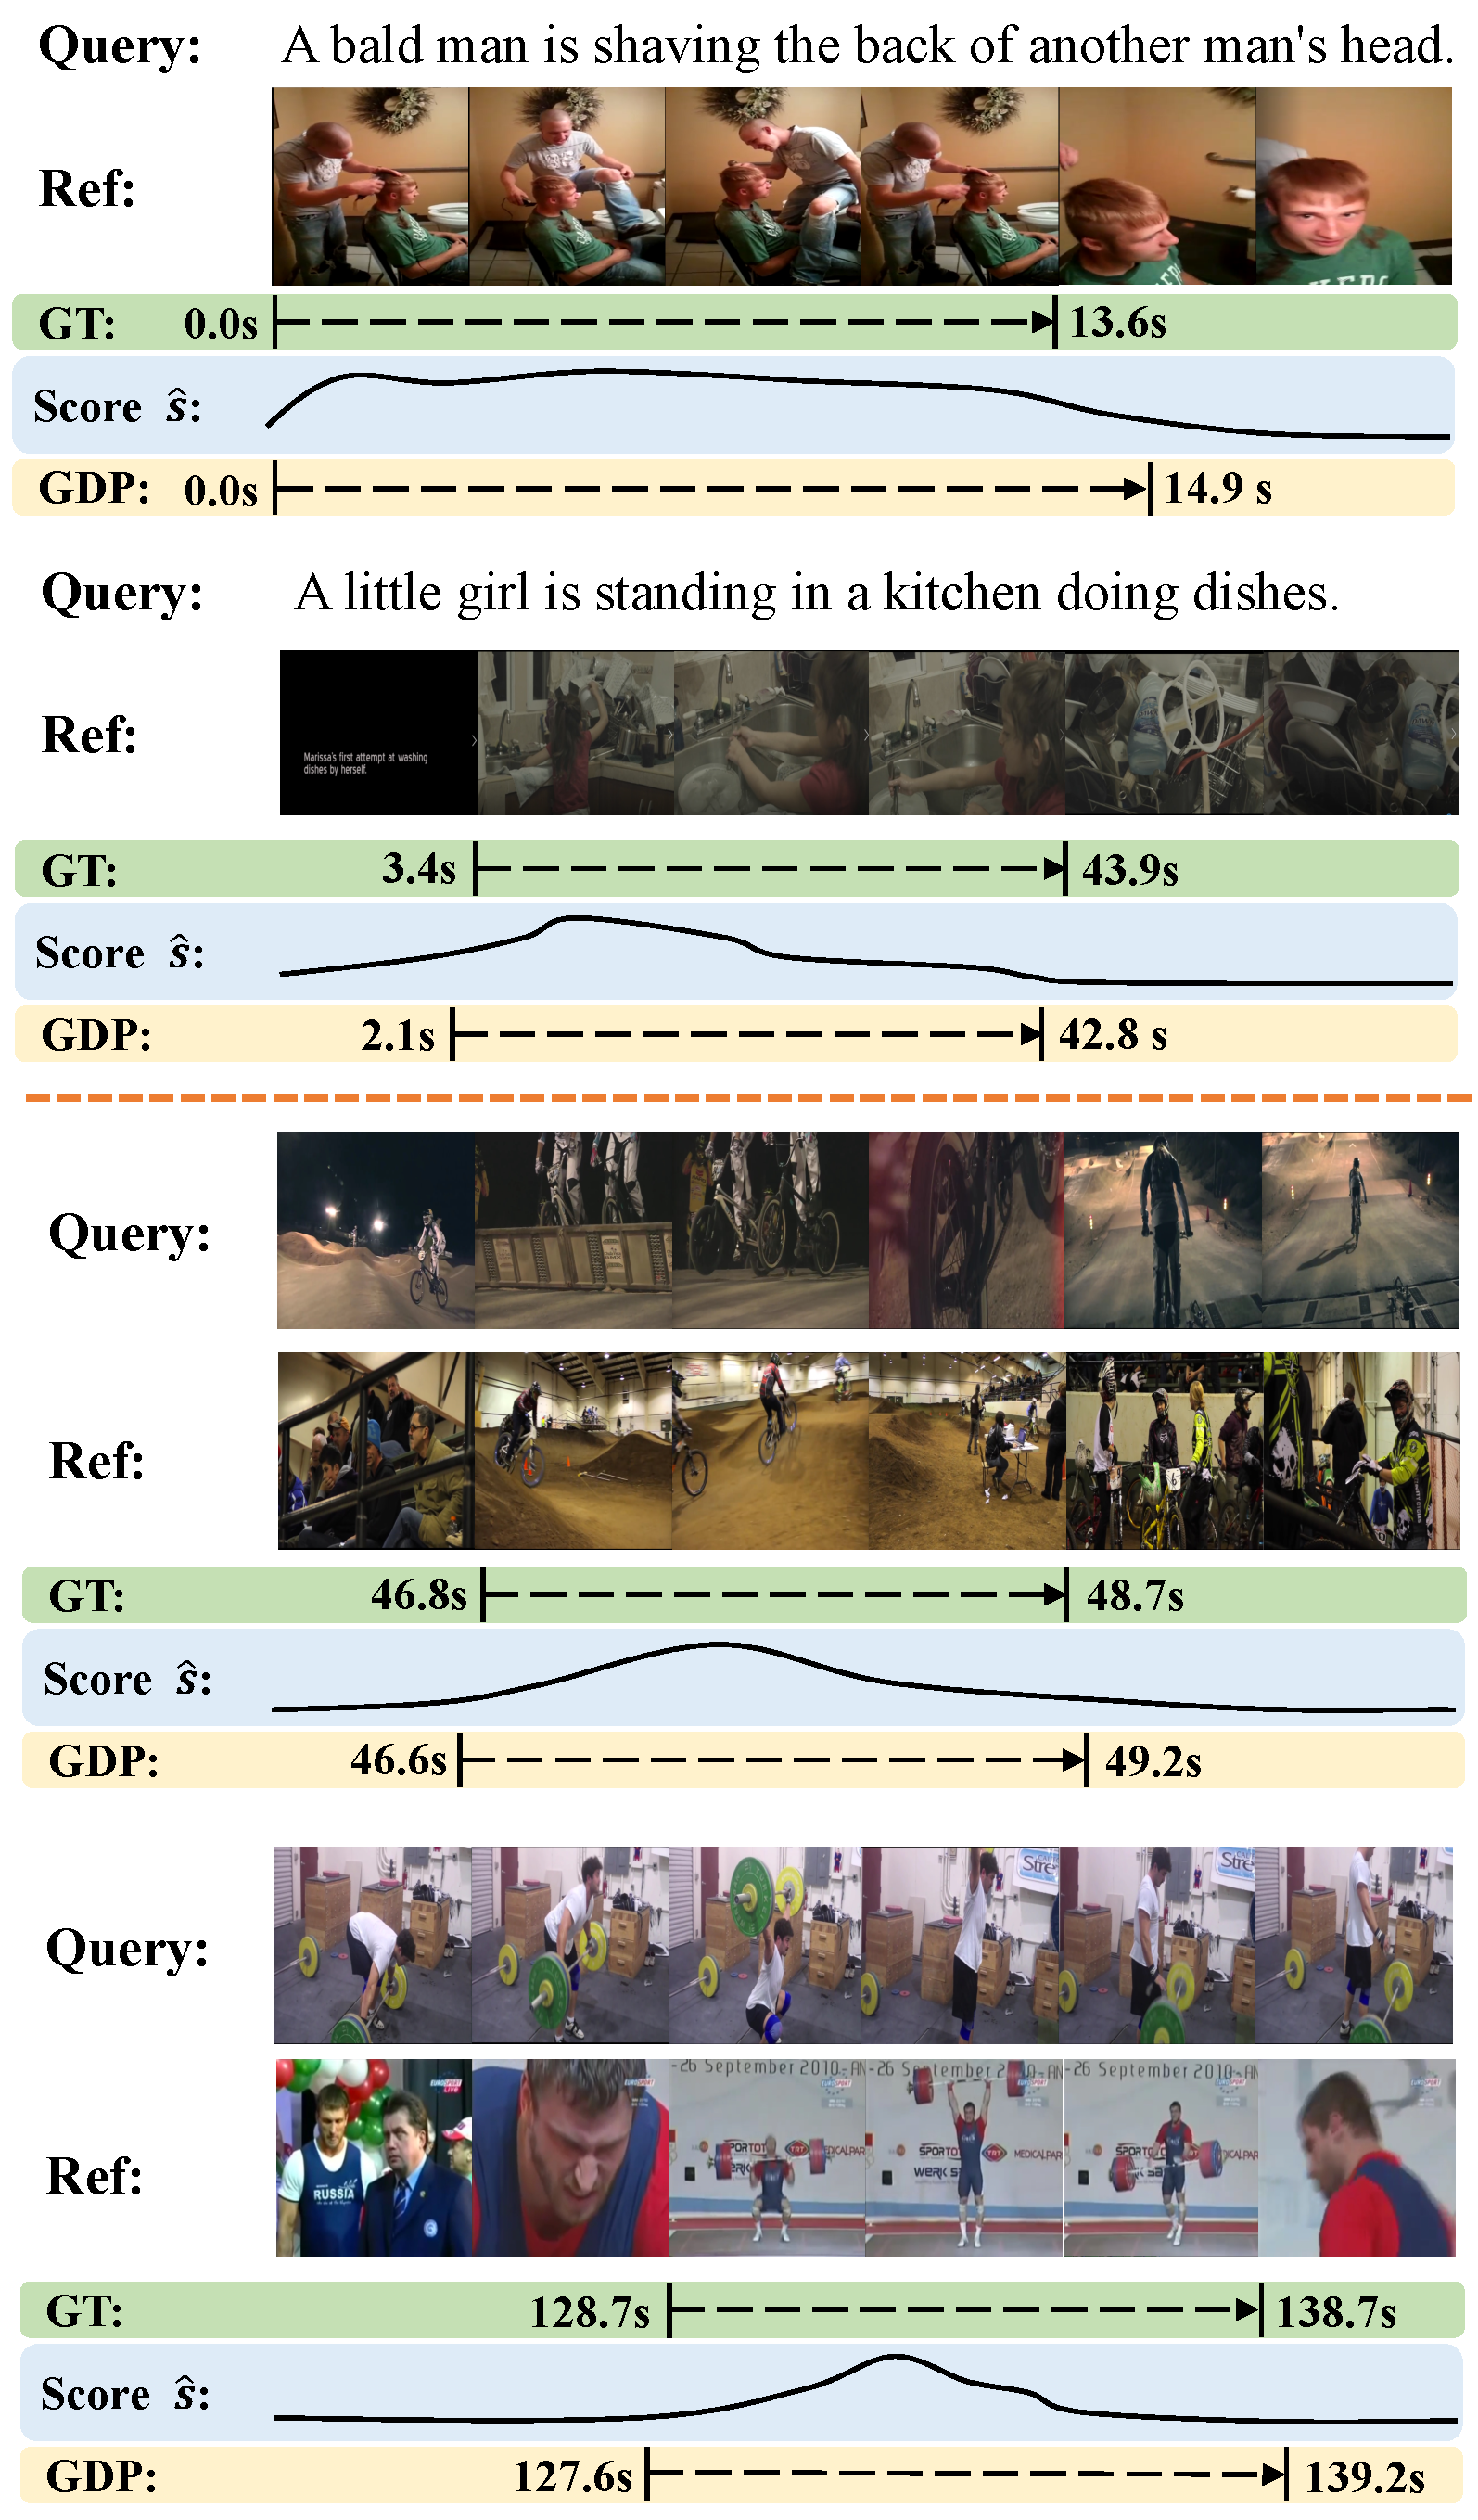
\includegraphics[width=0.6\linewidth]{chapter6/res/qualtative_results.pdf}
    \caption{GDP模型分别在ActivityNet Captions和Activity-VRL的检索结果}
    \label{ch6:fig:qualtative_results}
\end{figure}


%%%%%%%%%%%%%%%%%%% SOTA NLVL %%%%%%%%%%%%%%%%%%%%%%%
\begin{table*}[tbp]
    \centering
    \scalebox{0.75}{
        \begin{tabular}{|l|l| c c c| c c c | c c c |}
            \hline
            & \multirow{2}{*}{Method} & \multicolumn{3}{c|}{TACoS} & \multicolumn{3}{c|}{Charades-STA} & \multicolumn{3}{c|}{ActivityNet Captions} \\
            & & IoU@0.1 & IoU@0.3 & mIoU & IoU@0.3 & IoU@0.5 & IoU@0.7 & IoU@0.3 & IoU@0.5 & mIoU  \\
            \hline
            \parbox[t]{2mm}{\multirow{10}{*}{\rotatebox[origin=c]{90}{TD}}} & VSA-RNN & 8.84 & 6.91 & - & - & 10.50 & 4.32 & - & - & - \\
            & VSA-STV & 15.01 & 10.77 & - & - & 16.91 & 5.81 & - & - & - \\
            & CTRL & 24.32 & 18.32 & - & - & 23.63 & 8.89 & - & - & - \\
            & ROLE & - & - & - & 25.26 & 12.12 & - & - & - & - \\
            & ACRN & 24.22 & 19.52 & - & - & - & - & - & - & - \\
            & MCF & 25.84 & 18.64 & - & - & - & - & - & - & - \\
            & TGN & - & - & - & - & - & - & 43.81 & 27.93 & - \\
            & ACL & 28.31 & 22.07 & - & - & 26.47 & 11.23 & - & - & - \\
            & SAP & 31.15 & - & - & - & 27.42 & 13.36 & - & - & - \\
            & QSPN & - & - & - & \textbf{54.70} & 35.60 & 15.80 & 45.30 & 27.70 & - \\
            \cline{1-2}
            \parbox[t]{2mm}{\multirow{2}{*}{\rotatebox[origin=c]{90}{RL}}} & RWM & - & - & - & - & 36.70 & - & - & 36.90 & - \\
            & SM-RL & 26.51 & 20.25 & - & - & 24.36 & 11.17 & - & - & - \\
            \cline{1-2}
            \parbox[t]{2mm}{\multirow{4}{*}{\rotatebox[origin=c]{90}{BU}}} & L-NET & - & - & 13.41 & - & - & - & - & - & - \\
            & ABLR-aw & 31.60 & 18.90 & 12.50 & - & - & - & 53.65 & 34.91 & 35.72 \\
            & ABLR-af & 34.70 & 19.50 & 13.40 & - & - & - & 55.67 & 36.79 & 36.99 \\
            & \textbf{GDP} & \textbf{39.68} & \textbf{24.14} & \textbf{16.18} & 54.54 & \textbf{39.47} & \textbf{18.49} & \textbf{56.17} & \textbf{39.27} & \textbf{39.80} \\
            \hline
        \end{tabular}
    }
    \caption{不同基于语句查询的视频片段检索方法的性能对比}
    \label{ch6:tab:sota_nlvl}
\end{table*}

%%%%%%%%%%%%%%%%%%%%% SOTA VRL %%%%%%%%%%%%%%%%%%%%%%%
\begin{table}[tbp]
    \centering
    \scalebox{0.9}{
        \begin{tabular}{|l| c c c c c c |}
            \hline
            mAP@1 & 0.5 & 0.6 & 0.7 & 0.8 & 0.9 & Avg   \\
            \hline
            Frame-level  & 18.8 & 13.9 & 9.6 & 5.0 & 2.3 & 9.9 \\
            Video-level & 24.3 & 17.4 & 12.0 & 5.9 & 2.2 & 12.4 \\
            SST & 33.2  & 24.7 & 17.2 & 7.8 & 2.7 & 17.1  \\
            CGBM & 43.5 & 35.1 & 27.3 & 16.2 & 6.5 & 25.7 \\
            \textbf{GDP} & \textbf{44.0} & \textbf{35.4} & \textbf{27.7} & \textbf{20.0} & \textbf{12.1} & \textbf{27.8} \\
            \hline
        \end{tabular}
    }
    \caption{不同基于视频查询的视频片段检索方法的性能对比}
    \label{ch6:tab:sota_vrl}
\end{table}


\subsection{视频片段检索性能对比}

\textbf{\kaishu{基于语句查询的视频片段检索}}:在本节,我们将本章提出的GDP模型与目前最先进的基于语句查询的视频片段检索方法进行对比。按照自顶向下和自底向上框架划分,这些方法可以分为三类:(1)自顶向下模型:\textbf{VSA-RNN}~\cite{gao2017tall}、\textbf{VSA-STV}~\cite{gao2017tall}、\textbf{CTRL}~\cite{gao2017tall}、\textbf{ROLE}~\cite{liu2018cross}、\textbf{ACRN}~\cite{liu2018attentive}、\textbf{MCF}~\cite{wu2018multi}、\textbf{TGN}~\cite{chen2018temporally}、\textbf{ACL}~\cite{ge2019mac}、\textbf{SAP}~\cite{chen2019semantic}和\textbf{QSPN}~\cite{xu2019multilevel}。(2)基于强化学习的模型:\textbf{RWM}~\cite{he2019read}、\textbf{SM-RL}~\cite{wang2019language}。(3)自底向上模型:\textbf{L-Net}~\cite{chen2019localizing}、\textbf{ABLR-af}、\textbf{ABLR-aw}~\cite{yuan2019find}。

表~\ref{ch6:tab:sota_nlvl}展示了GDP模型的定量实验结果。从表~\ref{ch6:tab:sota_nlvl}可以看出,GDP在所有的数据集下都可以达到目前最好的性能。尤其对于更加严格的评价指标,性能增益往往更加明显。例如,在数据集TACoS和ActivityNet Captions中,mIoU可以分别提升2.77\%和2.81\%;在数据集Charades-STA中,IoU@0.7可以提升2.69\%。

图~\ref{ch6:fig:qualtative_results}展示了GDP模型的定性实验结果。由图~\ref{ch6:fig:qualtative_results}可以看出,置信度最高的视频帧往往都接近于人工标注的检索片段中心位置,这也符合我们的模型设计初衷,将检索片段中心帧的置信分数设为最高。


\textbf{\kaishu{基于视频查询的视频片段检索}}:在本节,我们将本章提出的GDP模型与目前最先进的基于视频查询的视频片段检索方法进行对比。同样,我们可以将这些方法分为两类:(1)自顶向下模型:\textbf{Frame-level}~\cite{feng2018video}、\textbf{video-level}~\cite{feng2018video}、\textbf{SST}~\cite{buch2017sst}。(2)自底向上模型:\textbf{CGBM}~\cite{feng2018video}。

从表~\ref{ch6:tab:sota_vrl}可以看出,GDP模型在所有的评价指标下都超过目前最好的模型。尤其对于高质量的预测,性能增益更加明显。例如:在tIoU阈值为0.9时,GDP的性能相比提升接近100\%。


\begin{figure}[tbp]
    \centering
    \includegraphics[width=0.9\linewidth]{chapter6/res/ablative_backbone.pdf}
    \caption{同一骨干网络不同特征优化层的性能对比}
    \label{ch6:fig:ablative_backbone}
\end{figure}


\subsection{视频片段检索性能分析}

\textbf{\kaishu{图特征金字塔层的有效性}}:为了验证图特征金字塔层的有效性,我们设计了三种基准模型进行对比。如图~\ref{ch6:fig:ablative_backbone}所示,模型A(a)包含一个骨干网络和一个密集头网络;模型B(b)用骨干网络的输出特征序列构建一个特征金字塔,然后直接将不同尺度的特征直接进行拼接融合;模型C(c)参考FPN(Feature Pyramid Network)~\cite{lin2017feature}使用一个自顶向下的支路网络将不同尺度的特征进行融合;模型D(d)为GDP模型。其中,四个对比模型中的骨干网络和密集头网络结构都完全相同。

%%%%%%%%%% Ablation about Backbone NLVL %%%%%%%%%%%%%%%%
\begin{table*}[t]
    \centering
    \scalebox{0.9}{
        \begin{tabular}{|c | c c c c| c c c c| c c c c|}
            \hline
            & \multicolumn{4}{c|}{TACoS} & \multicolumn{4}{c|}{Charades-STA} & \multicolumn{4}{c|}{ActivityNet Captions}  \\
            \hline
            \multirow{2}{*}{Model} & \multicolumn{3}{c|}{IoU@} & \multirow{2}{*}{mIoU} & \multicolumn{3}{c|}{IoU@} & \multirow{2}{*}{mIoU} & \multicolumn{3}{c|}{IoU@} & \multirow{2}{*}{mIoU} \\
            & 0.1 & 0.3 & 0.5 & \multicolumn{1}{|c|}{} & 0.3 & 0.5 & 0.7 & \multicolumn{1}{|c|}{}  & 01. & 0.3 & 0.5 & \multicolumn{1}{|c|}{} \\
            \hline
            A & 37.4 & 23.3 & 11.5 & 15.3 & 51.8 & 38.3 & 17.8 & 35.1 & 72.1 & 56.0 & \textbf{40.7} & 39.3  \\
            B & 37.3 & 23.1 & \textbf{13.9} & 15.8 & 53.8 & 38.6 & 18.4 & 36.0 & 73.1 & 56.2 & 40.3 & 39.5  \\
            C & 36.8 & 23.1 & 13.8 & 15.7  & 52.6 & 38.9 & 18.3 & 35.8 & 73.7 & 54.7 & 38.9 & 39.4 \\
            D & \textbf{39.7} & \textbf{24.1} & 13.5 & \textbf{16.2} & \textbf{54.5} & \textbf{39.5} & \textbf{18.5} & \textbf{36.6} & \textbf{75.0} & \textbf{56.2} & 39.3 & \textbf{39.8} \\
            \hline
        \end{tabular}
    }       
    \caption{基于语句查询的视频片段检索任务中模型A、B、C、D的性能对比}
    \label{ch6:tab:nlvl_ablation_backbone}
\end{table*}

%%%%%%%%%% Ablation about Backbone VRL %%%%%%%%%%%%%%%
\begin{table*}[t]
    \centering
    \scalebox{0.9}{
        \begin{tabular}{|c |c c c c c|}
            \hline
            mAP@1 & 0.5 & 0.6 & 0.7 & 0.8 & 0.9 \\
            \hline
            A & 41.1 & 34.2 & 27.7  & \textbf{20.3} & 6.8 \\
            B & 43.3 & 35.0 & \textbf{27.9} & 18.2  & 9.6 \\
            C & 42.9 & 34.5 & 26.9 & 18.8  & 8.4 \\
            D & \textbf{44.0} & \textbf{35.4} & 27.7 & 20.0 & \textbf{12.1} \\
            \hline
        \end{tabular}
    }       
    \caption{基于视频查询的视频片段检索任务中模型A、B、C、D的性能对比}
    \label{ch6:tab:vrl_ablation_backbone}
\end{table*}

\begin{figure}[t]
    \centering
    \includegraphics[width=0.9\linewidth]{chapter6/res/node_visualization.pdf}
    \caption{场景空间中的节点可视化}
    \label{ch6:fig:node_visualization}
\end{figure}

基于语句查询和视频查询的视频片段检索的结果分别展示在表~\ref{ch6:tab:nlvl_ablation_backbone}和表~\ref{ch6:tab:vrl_ablation_backbone}中。根据实验结果,我们可以发现:(1)特征金字塔结构可以显著地提升视频片段检索任务的性能(即:模型B、C、D的性能明显好于模型A的性能)。(2)利用自顶向下的支路将连续两个尺度的特征进行融合并不能有效地融合多尺度特征。例如,模型B和模型C的性能十分接近,即自顶向下支路和直接拼接效果接近。(3)GDP模型(模型D)在绝大多数的数据集和评价指标下都能取得最好的结果,说明了图特征金字塔层对视频检索任务的有效性。


%%%%%%%%%%%%%%%% Ablation Head Network %%%%%%%%%%%%%%
\begin{table}[t]
    \centering
    \scalebox{0.9}{
        \begin{tabular}{|l|l| c c c|}
            \hline
            Dataset & Metric & Sparse & Dense$^*$ & Dense \\
            \hline
            \multirow{4}{*}{TACoS} & IoU@0.1 & 32.3 & 36.5 & \textbf{39.7} \\
            & IoU@0.3 & 18.7 & 22.9 & \textbf{24.1}  \\
            & IoU@0.5 & 9.6 & 13.0 & \textbf{13.5}  \\
            & mIoU & 12.9 & 15.2 & \textbf{16.2}  \\
            \cline{1-5}
            \multirow{4}{*}{Charades-STA} & IoU@0.3 & 52.9 & 53.9 & \textbf{54.5} \\
            & IoU@0.5 & 31.4 & 39.0 & \textbf{39.5}   \\
            & IoU@0.7 & 14.7 & 18.3 & \textbf{18.5} \\
            & mIoU & 35.1 & 36.1 & \textbf{36.6}  \\
            \cline{1-5}
            \multirow{4}{*}{ActivityNet Captions} & IoU@0.1 & 72.4 & 73.5 & \textbf{75.0}  \\
            & IoU@0.3 & 53.0 & 55.9 & \textbf{56.2} \\
            & IoU@0.5 & 37.5 & \textbf{39.8} & 39.3  \\
            & mIoU & 39.0 & 39.3 & \textbf{39.8}  \\
            \hline
            \multirow{6}{*}{ActivityNet-VRL} & tIoU@0.5 & 41.6 & 42.3 & \textbf{44.0}  \\
            & tIoU@0.6 & 30.5 & 35.3 & \textbf{35.4}   \\
            & tIoU@0.7 & 25.7 & 27.6 & \textbf{27.7} \\
            & tIoU@0.8 & 19.8 & \textbf{20.6} & 20.0 \\
            & tIoU@0.9 & 8.5 & \textbf{12.5} & 12.1 \\
            & Average & 25.2 & 27.7 & \textbf{27.8}  \\
            \hline
        \end{tabular}
    }
    \caption{密集型头网络和稀疏型头网络的性能对比}
    \label{ch6:tab:ablation_head}
\end{table}


\textbf{\kaishu{密集头网络的有效性}}:为了评估密集头网络的有效性,我们设计了一个基准模型:它使用和GDP完全相同的骨干网络和图卷积特征层,然后只是将密集头网络替换成稀疏型头网络,即直接预测两端边界的概率。

基于语句查询和视频查询的视频片段检索的结果展示在表~\ref{ch6:tab:ablation_head}中,其中Sparse表示基准模型(稀疏型头网络),Dense$^*$表示模型在测试阶段没有使用时域池化。由表~\ref{ch6:tab:ablation_head}可以看出,密集头网络可以显著提升模型性能。尤其对于长视频(如:数据集TACoS),性能提升更加明显。这也间接说明密集头网络能够缓解稀疏头网络中存在的正负训练样本极度不均等问题。


\textbf{\kaishu{场景空间节点的可视化}}:在图~\ref{ch6:fig:node_visualization}中,我们随机选取了同一个尺度下的四个节点,然后每个节点选取了三个视频帧来表示节点信息。如图~\ref{ch6:fig:node_visualization}所示,同一个节点中的视频帧通常包含一个特定的视觉场景或相似的场景内容。

\section{本章小结}
在本章,我们深入分析了目前视频片段检索方法的优缺点,并针对稀疏型自底向上框架的设计缺点,提出了一种全新的密集型自底向上网络:基于图特征金字塔的密集型预测(GDP)。GDP通过引入一个图特征金字塔层来充分编码视频中多个场景之间的内在联系,提升特征帧序列的表达能力。同时,GDP将目前的稀疏头网络替换成密集头网络,不仅可以避免训练过程中正负样本极度不均的问题,同时可以将动作边界预测问题分解成相关性预测和动作边界回归两个子问题,简化视频片段检索的难度。在两种不同的查询形式下(基于自然语句和视频片段)的视频片段检索任务中,GDP模型都能取得目前最好的性能。


\chapter{基于反事实样本生成的图像视觉问答方法}

随着深度学习技术的发展,虽然图像视觉问答技术已经取得了长足的进步,但是目前的图像视觉问答模型往往只依赖于问题与答案之间的联系(即文本偏置)。为了缓解这一问题,最近的一些图像视觉问答模型开始引入一个辅助网络来约束目标视觉问答模型的训练,并且在标准图像视觉问答数据集VQA-CP上取得了目前最好的实验性能。然而,由于模型设计的复杂性,这类复合模型难以满足一个理想视觉问答模型应该具备的两个特点:1)视觉可解释性:在预测答案时,模型应该关注正确的视觉图像区域;2)文本敏感性:在变换问题时,模型应该感知问题的变化。因此,本章提出了一种通用的反事实样本生成机制(Counterfactual Samples Synthesizing, CSS)。CSS通过遮盖图像中的重要区域或问题中的重要单词来生成新的训练样本,然后对这些样本赋予不同的标准答案。通过使用原始训练样本和新生成训练样本一起对模型进行训练,迫使模型能够关注被遮盖的重要区域和重要单词,提升模型的视觉可解释性和文本敏感性。同样,模型的性能会被进一步提升。大量的对比实验证明CSS的有效性。值得注意的是,当对目前最好的视觉问答模型LMH~\cite{clark2019don}使用CSS机制生成样本一起训练后,模型在数据集VQA-CP v2上可以取得58.95\%的准确率,提升6.5\%。

\section{问题描述} \label{ch7:sec:introduction}
图像视觉问答(Visual Question Answering, VQA)是场景推理中一个重要的任务,也是走向真正人工智能时代至关重要的一步。图像视觉问答任务是给定一个图像和问题,模型需要根据图像内容问题回答。随着大规模视觉问答数据集的出现(如:VQA v1~\cite{antol2015vqa}和VQA v2~\cite{goyal2017making}),视觉问答任务得到了前所未有的关注。然而,由于在真实图像数据集的标注过程中不可避免地会引入偏置,目前的图像视觉问答模型往往过于依赖问题和答案之间的联系(即文本偏置)~\cite{agrawal2016analyzing,zhang2016yin,johnson2017clevr,goyal2017making}。例如,对于所有“How many”开始的问题,模型都回答“2”也可以得到较好的实验结果。为了去除之前视觉问答数据集中的偏置对视觉问答研究的影响,近期,学术界提出了一个新的数据集VQA-CP(VQA under Changing Priors)~\cite{agrawal2018don}。VQA-CP通过故意让训练集和测试集中问题和答案的分布不同,让过于依赖文本偏置的模型得到较差的实验结果。许多的视觉问答模型在VQA-CP数据集上都出现了明显的性能下降~\cite{andreas2016neural,fukui2016multimodal,yang2016stacked,anderson2018bottom}。

\begin{figure}[t]
    \centering
        \includegraphics[width=0.8\linewidth]{chapter7/res/motivation.pdf}
    \caption{VQA模型必备的视觉可解释性和文本敏感性}
    \label{ch7:fig:motivation}
\end{figure}

目前,对于数据集VQA-CP来说,最好的解决方案都是基于复合模型的设计,即引入一个辅助网络来约束视觉问答网络的训练,其中的辅助网络只用文本(即问题语句)作为输入。具体来说,这些复合模型又可以细分为两个小类:1)基于对抗学习的方法~\cite{ramakrishnan2018overcoming,grand2019adversarial,belinkov2019don}:它们使用对抗学习~\cite{goodfellow2014generative}的方式来训练这两个网络,即减少视觉问答网络的损失函数,而增大辅助网络的损失函数。因为这两个模型共享同一个文本编码器,这类基于对抗学习的方法希望通过学习到没有偏置的文本编码向量来缓解模型过于依赖文本偏置的问题。然而,有实验表明,这类方法在计算梯度过程中引入大量噪声,造成训练过程不稳定。2)基于融合的方法~\cite{cadene2019rubi,clark2019don,mahabadi2019simple}:它们将两个网络预测答案的概率分布进行融合,然后根据融合后的概率分布计算训练梯度。这类方法的设计思想是让视觉问答网络更加关注到辅助网络无法回答的训练样本。

尽管复合模型在数据集VQA-CP上取得了最好的实验性能,但是由于目前的复合模型复杂的设计,使得这类模型难以满足一个理想视觉问答模型应该具体的两个特点:1)\textbf{视觉可解释性}:在预测答案时,模型应该关注正确的视觉图像区域~\cite{ross2017right}。如图~\ref{ch7:fig:motivation}(a)所示,尽管两个模型都可以预测出正确的答案“surfing”,但实际上两个模型是根据完全不同的视觉区域做的决策。2)\textbf{文本敏感性}:在变换问题时,模型应该感知问题的变化。如图~\ref{ch7:fig:motivation}(b)所示,当两个问题的句式结构十分接近时(如只替换“luggage”成“bus”),如果问句的意思完全不同,模型应该感知问题的差异变化,然后做出不同的预测。

\begin{figure}[t]
    \centering
        \includegraphics[width=0.8\linewidth]{chapter7/res/V-CSS_Q-CSS.pdf}
    \caption{V-CSS和Q-CSS示意图}
    \label{ch7:fig:V-CSS_Q-CSS}
\end{figure}

在本文,我们提出了一个全新的反事实样本生成机制(CSS),CSS可以“即插即用”地提升多种图像视觉问答模型的视觉可解释性和文本敏感性。如图~\ref{ch7:fig:V-CSS_Q-CSS}所示,CSS包含两种不同的样本生成机制:V-CSS和Q-CSS。对于V-CSS,我们通过遮盖图像中的重要区域,得到反事实图像。所谓的“重要区域”是指针对回答该问题非常重要的图像区域。得到的反事实图像和原始的问题就组成了一个新的图像问题对。对于Q-CSS,我们通过将原始问题中的重要单词替换成一个特定的词“[MASK]”得到反事实问题。同样,反事实问题和原始的图像也组成了一个新的图像问题对。给定一个图像问题对,一个标准的视觉问答训练样本同时还需要标准答案。为了避免大量的人工标准,我们设计了一个动态的答案生成机制,对所有新合成的图像问题对分配合理的“标准”答案(如:图~\ref{ch7:fig:V-CSS_Q-CSS}中的“not green”)。然后通过使用原始训练样本和新生成训练样本一起对模型训练,迫使模型能够关注被遮盖的重要区域和重要单词。


我们通过大量的定性实验和定量实验都验证了CSS的有效性。CSS可以无缝地用在复合模型中,不仅提升它们的视觉可解释性和文本敏感性,同时提升模型在VQA-CP上的实验性能。值得注意的是,当对目前最好的视觉问答模型LMH~\cite{clark2019don}使用CSS机制生成样本一起训练后,我们在VQA-CP v2数据集上得到58.95\%的准确率。

\section{反事实样本生成}

对于图像视觉问答任务,我们参考现有的工作将其看成一个多类别分类任务。为了不失一般性,给定一个视觉问答数据集$\mathcal{D} = \{I_i, Q_i, a_i \}^N_i$包含大量的图像$I_i \in \mathcal{I}$、问题$Q_i \in \mathcal{Q}$和答案$a_i \in \mathcal{A}$,视觉问答任务的目的在于学习一个映射函数,$f_{vqa}: \mathcal{I} \times \mathcal{Q} \rightarrow [0, 1]^{|\mathcal{A}|}$,对任意的图像问题对可以预测一个答案概率分布。为了简洁,我们在后续的表述中省略下角标$i$。

在本节,我们先介绍基本的自底向上和自顶向下模型~\cite{anderson2018bottom},以及复合模型(第~\ref{ch7:sec:preliminaries}节);其次,我们介绍CSS的具体细节(第~\ref{ch7:sec:css}节)。

\subsection{引言} \label{ch7:sec:preliminaries}

\textbf{自底向上和自顶向下模型}(Bottom-Up Top-Down, UpDn):对于每张图像$I$,UpDn模型使用图像编码器$e_v$将图像编码成一系列物体特征:$\bm{V} = \{\bm{v}_1, ..., \bm{v}_{n_v}\}$,其中$\bm{v}_i$表示第$i$个物体特征。对于每个问题$Q$,UpDn模型使用问题编码器$e_q$编码成一系列单词特征:$\bm{Q} = \{\bm{w}_1, ..., \bm{w}_{n_q}\}$,其中$\bm{w}_j$表示第$j$个单词的特征。然后特征$\bm{V}$和$\bm{Q}$都输入到模型$f_{vqa}$中来预测答案概率分布:
\begin{equation} \label{ch7:eq:p_vqa}
    P_{vqa}(\bm{a}|I, Q) = f_{vqa}(\bm{V}, \bm{Q})
\end{equation}
其中,模型$f_{vqa}$通常包含一个注意力机制,然后利用交叉熵作为损失函数对模型进行优化。

\textbf{复合模型}:由前文提到(第~\ref{ch7:sec:introduction}节)提到,复合模型主要细分为两小类:基于对抗学习的方法和基于融合的方法。因为基于对抗学习的方法~\cite{ramakrishnan2018overcoming,grand2019adversarial,belinkov2019don}训练过程不稳定,在本节,我们只介绍基于融合的方法~\cite{cadene2019rubi,clark2019don,mahabadi2019simple}。如算法~\ref{ch7:alg:VQA},它们通过引入辅助网络$f_q$,只利用问题$\bm{Q}$做为输入:
\begin{equation}
P_{q}(\bm{a}|Q) = f_{q}(\bm{Q})
\end{equation}
然后,它们通过一个融合函数$M$将两个网络的概率分布进行融合:
\begin{equation}
\hat{P}_{vqa}(\bm{a}|I, Q) = M(P_{vqa}(\bm{a}|I, Q), P_{q}(\bm{a}|Q))
\end{equation}
在训练阶段,直接基于融合后的答案分布$\hat{P}_{vqa}(\bm{a})$计算交叉熵损失,然后计算梯度优化$f_{vqa}$和$f_q$。在测试阶段,只使用模型$f_{vqa}$。

\begin{algorithm}[t]
    \caption{复合模型(基于融合的方法)}\label{ch7:alg:VQA}
    \begin{algorithmic}[1]
        \Function {$\mathcal{\textcolor{blue}{VQA}}$}{$I, Q, a, cond$}
        \State $ \bm{V} \leftarrow e_v(I) $
        \State $ \bm{Q} \leftarrow e_q(Q) $
        \State $ P_{vqa}(\bm{a}) \leftarrow f_{vqa}(\bm{V}, \bm{Q}) $
        \State $ P_{q}(\bm{a}) \leftarrow f_{q}(\bm{Q})$      \Comment{辅助模型}
        \State $ \hat{P}_{vqa}(\bm{a}) \leftarrow M(P_{vqa}(\bm{a}), P_{q}(\bm{a}))  $
        \State $ Loss \leftarrow \text{XE}(\hat{P}_{vqa}(\bm{a}), a)$ \Comment{参数更新}
        \If{$cond$}
        \State \textbf{return} $\bm{V}, \bm{Q}, P_{vqa}(\bm{a})$
        \EndIf 
        \EndFunction
    \end{algorithmic}
\end{algorithm}

\subsection{反事实样本生成} \label{ch7:sec:css}
整个反事实样本生成(CSS)算法的流程展示在算法~\ref{ch7:alg:CSS}。具体来说,对于给定的一个视觉问答模型(即$\mathcal{VQA}$)和训练样本$(I, Q, a)$,CSS主要包含三个步骤:

\begin{asparaenum}
\item 用原始的训练样本对$\mathcal{\textcolor{blue}{VQA}}$模型进行训练;

\item 用V-CSS生成反事实样本$(I^-, Q, a^-)$或用Q-CSS生成反事实样本$(I, Q^-, a^-)$;

\item 用新生成的反事实样本对$\mathcal{\textcolor{blue}{VQA}}$模型进行训练。
\end{asparaenum}

在接下来,我们先详细介绍两种反事实样本生成机制:V-CSS和Q-CSS。如算法~\ref{ch7:alg:CSS}所示,对于每个训练样本,我们只使用特定的一种样本生成机制,其中$\delta$是一个超参数来权衡两种生成机制的比例。


\begin{algorithm}[tbp]
    \caption{反事实样本生成}\label{ch7:alg:CSS}
    \begin{algorithmic}[1]
        \Function {$\mathcal{CSS}$}{$I, Q, a$}
        \State $ \bm{V}, \bm{Q}, P_{vqa}(\bm{a}) \leftarrow \mathcal{\textcolor{blue}{VQA}}(I, Q, a, \text{True})$
        \State $ cond \sim U[0, 1]$
        \If {$cond \geq \delta $}  \Comment{执行V-CSS}
            \State $ \mathcal{I} \leftarrow  \textsc{IO\_Sel}(I, Q) $
            \State $ s(a, \bm{v}_i) \leftarrow \mathcal{S}(P_{vqa}(a), \bm{v}_i)$
            \State $ I^+, I^- \leftarrow \textsc{CO\_Sel}(\mathcal{I}, \{s(a, \bm{v}_i) \}) $
            \State $ a^- \leftarrow \textsc{DA\_Ass}(I^+, Q, \mathcal{VQA}, a) $
            \State $ \mathcal{\textcolor{blue}{VQA}}(I^-, Q, a^-, \text{False})$
        \Else \Comment{执行Q-CSS}
            \State $ s(a, \bm{w}_i) \leftarrow \mathcal{S}(P_{vqa}(a), \bm{w}_i) $
            \State $ Q^+, Q^- \leftarrow \textsc{CW\_Sel}(\{s(a, \bm{w}_i)\})$
            \State $ a^- \leftarrow \textsc{DA\_Ass}(I, Q^+, \mathcal{VQA}, a) $
            \State $ \mathcal{\textcolor{blue}{VQA}}(I, Q^-, a^-, \text{False})$
        \EndIf
        \EndFunction
    \end{algorithmic}
\end{algorithm}


\textbf{V-CSS}:我们将按照程序执行顺序陆续介绍V-CSS的主要步骤(即算法~\ref{ch7:alg:CSS}中第5行-第8行):初始物体选择(\textsc{IO\_Sel})、物体局部贡献计算、重要物体选择(\textsc{CO\_Sel})和动态答案生成(\textsc{DA\_Ass}):

初始物体选择(\textsc{IO\_Sel}):通常给定一个图像问题对$(Q, a)$,图像中只有部分物体与当前问题有关。为了缩小后续重要物体选择的范围,我们首先构建一个小的物体集$\mathcal{I}$,使得物体集$\mathcal{I}$中的物体都可能对回答正确问题有帮助。因为缺乏人工的标注,我们参考Wu等人~\cite{wu2019self}先提取与问答语句十分相关的物体。具体来说,我们先用spaCy POS tagger~\cite{honnibal2017spacy}提取问答中的所有名词,然后利用所有名词和类别的GloVe编码~\cite{pennington2014glove}计算余弦相似度,其中相似度记为$\mathcal{SIM}$。之后根据$\mathcal{SIM}$选择分数最高的$|\mathcal{I}|$个物体作为$\mathcal{I}$。

物体局部贡献计算:当得到物体集$\mathcal{I}$之后,我们开始计算每个物体对最终的正确答案的局部贡献。我们参考现有的工作~\cite{jain2019attention,selvaraju2019taking,wu2019self},同样使用修改的Grad-CAM~\cite{selvaraju2017grad}算法来计算局部贡献。对于第$i$个物体来说,它对正确答案$a$的贡献为:
\begin{equation} \label{ch7:eq:eq_4}
s(a, \bm{v}_i) = \mathcal{S}(P_{vqa}(a), \bm{v}_i) \coloneqq (\nabla_{\bm{v}_i} P_{vqa}(a))^T\mathbf{1}
\end{equation}
其中$P_{vqa}(a)$表示对正确答案$a$的预测概率,$\bm{v}_i$表示第$i$个物体特征,$\mathbf{1}$表示向量所有元素都为1。显然,如果分数$s(a, \bm{v}_i)$越高,物体特征$\bm{v}_i$对正确答案$a$的贡献也越大。

重要物体选择(\textsc{CO\_Sel}):在对物体集$\mathcal{I}$中每个物体计算局部贡献$s(a, \bm{v}_i)$之后,我们将分数最大的前K个物体当成重要的物体,即$I^+$。对于每张图像,K是满足公式~\eqref{ch7:eq:eq_5}最小的数:
\begin{equation} \label{ch7:eq:eq_5}
\sum_{\bm{v}_i \in I^+} \exp(s(a, \bm{v}_i)) / \sum_{\bm{v}_j \in \mathcal{I}} \exp(s(a, \bm{v}_j))  > \eta
\end{equation}
其中$\eta$是一个常数,所有的实验中我们将$\eta$设定为0.65。然后反事实图像就是物体集$I^+$在所有物体$I$中的补集,即$I^- = I \backslash I^+$。图~\ref{ch7:fig:IQ+-}展示了一个$I$、$I^+$和$I^-$的示例。

动态答案生成(\textsc{DA\_Ass}):给定反事实图像$I^-$和原始问题$Q$,我们可以组成一个新的图像问题对($I^-, Q$)。作为训练样本,新的图像问题对同样需要分配标准答案。为了减少人工标准的成本,我们设计了一种动态的答案生成机制,预测一个标准答案$a^-$。动态答案生成机制的细节在算法~\ref{ch7:alg:daass}。具体来说,我们将另一个图像问题对($I^+, Q$)输入到视觉问答模型$\mathcal{VQA}$中,然后得到预测的答案概率分布$P^+_{vqa}(\bm{a})$。根据概率$P^+_{vqa}(\bm{a})$,我们选取前N个答案作为$a^+$,然后定义$ a^- \coloneqq \{a_i | a_i \in a, a_i \notin a^+ \}$。极端情况下,如果模型对于图像问题对($I^+, Q$)可以回答全部的正确答案,即$a \subset a^+$,则$a^-$为空集$\emptyset$。

\begin{algorithm}[tbp]
    \caption{动态答案生成}\label{ch7:alg:daass}
    \begin{algorithmic}[1]
        \Function {$\textsc{DA\_Ass}$}{$I^+, Q^+, \mathcal{VQA}, a$}
        \State  $\mathcal{VQA}$.eval() \Comment{不更新参数}
        \State  $ \_, \_, P_{vqa}^+(\bm{a}) \leftarrow \mathcal{VQA}(I^+, Q^+, a, \text{True}) $
        \State $ a^+ \leftarrow \text{top-N}(\text{argsort}_{a_i \in \mathcal{A}}(P_{vqa}^+(a_i)))$
        \State $ a^- \coloneqq \{a_i | a_i \in a, a_i \notin a^+ \} $ \Comment{$a$是标准答案集}
        \State \textbf{return} $a^-$
        \EndFunction
    \end{algorithmic}
\end{algorithm}

\begin{figure}[t]
    \centering
        \includegraphics[width=0.8\linewidth]{chapter7/res/IQ+-.pdf}
    \caption{$I^+$、$I^-$、$Q^+$和$Q^-$的示例图}
    \label{ch7:fig:IQ+-}
\end{figure}

\textbf{Q-CSS}: 对于Q-CSS,主要的步骤和V-CSS非常接近,除了没有初始物体选择(即\textsc{IO\_Sel})。按照算法执行的顺序(算法~\ref{ch7:alg:CSS}第11行至第14行),Q-CSS主要包含三步:单词局部贡献计算、重要单词选择(\textsc{CW\_Sel})和动态答案生成(\textsc{DA\_Ass})。

单词局部贡献计算:与V-CSS(公式~\eqref{ch7:eq:eq_4})相似,对于第$i$个单词来说,它对正确答案$a$的贡献为:
\begin{equation} \label{ch7:eq:eq_6}
s(a, \bm{w}_i) = \mathcal{S}(P_{vqa}(a), \bm{w}_i) \coloneqq (\nabla_{\bm{w}_i} P_{vqa}(a))^T\mathbf{1}
\end{equation}

重要单词选择(\textsc{CW\_Sel}):对于这步,我们首先提取每个问题$Q$的问题类别前缀,这些前缀直接使用数据集VQA-CP默认的问题类别前缀。然后对剩余的单词选择贡献最高的K个单词作为重要单词。反事实问句$Q^-$就是将问句$Q$中的重要单词替换成一个特殊字符“[MASK]”。图~\ref{ch7:fig:IQ+-}展示了一个$Q$、$Q^+$和$Q^-$的示例。

动态答案生成(\textsc{DA\_Ass}):这个动态答案生成步骤和V-CSS的完全相同,即算法~\ref{ch7:alg:daass}。对于Q-CSS,\textsc{DA\_Ass}的输入是图像问题对$(I, Q^+)$。


\section{实验设置与性能对比}

我们主要在数据集VQA-CP~\cite{agrawal2018don}的测试集上对模型性能进行验证。为了实验比较的完整性,我们同样在VQA v2~\cite{goyal2017making}的验证集上进行测试。关于模型的准确率,我们使用通用的VQA准确率计算方式~\cite{antol2015vqa}。为了实验比较的公平性,所有的实验都采取与UpDn模型~\cite{anderson2018bottom}相同的数据预处理。

\subsection{CSS对视觉问答的性能分析}

\textbf{CSS机制中不同超参数选择的影响}:我们通过大量的对比实验来分析V-CSS和Q-CSS中不同超参数对模型性能的影响。具体来说,所有的实验都是基于模型LMH~\cite{clark2019don}。实验结果展示在图~\ref{ch7:fig:ablative_studies}中。

V-CSS中初始物体选择$\mathcal{I}$的大小:不同$\mathcal{I}$的大小对实验性能的影响如图~\ref{ch7:fig:ablative_studies}(a)所示。随着$\mathcal{I}$的增加,模型的性能逐渐降低。

V-CSS中重要物体选择的数量:不同重要物体选择的数量对实验性能的影响如图~\ref{ch7:fig:ablative_studies}(a)所示。我们比较了动态选择K(公式~\ref{ch7:eq:eq_5})和预先固定一些常数(如:1、3或5)。从实验结果可知,动态选择K个中国物体可以得到最佳性能。

Q-CSS中重要单词选择的数量:不同重要单词选择的数量对实验性能的影响如图~\ref{ch7:fig:ablative_studies}(b)所示。从实验结果可知,只选择一个单词作为重要单词性能最好。

V-CSS和Q-CSS的比例$\delta$:不同$\delta$对实验性能的影响如图~\ref{ch7:fig:ablative_studies}(c)所示。从实验结果可知,$\delta = 0.5$性能最好。


\begin{figure*}[t]
    \centering
    \includegraphics[width=\linewidth]{chapter7/res/ablative_studies.pdf}
    \caption{\textbf{消融实验}:不同超参数对V-CSS和Q-CSS性能的影响}
    \label{ch7:fig:ablative_studies}
\end{figure*}


\textbf{CSS机制对模型的通用性}:因为本章提出的CSS训练机制可以适用于不同的VQA模型中。为了验证CSS对不同模型结构性能的有效性,我们将CSS机制应用于多种VQA模型中:\textbf{UpDn}~\cite{anderson2018bottom}、\textbf{PoE} (Product of Experts)~\cite{clark2019don,mahabadi2019simple}、\textbf{RUBi}~\cite{cadene2019rubi}、\textbf{LMH}~\cite{clark2019don}。特别地,模型PoE、RUBi、LMH属于复合模型。所有的实验结果展示在表~\ref{ch7:tab:boost_models},其中$^\dagger$表示我们的重现结果。

和不同VQA结构的基准模型对比,CSS同时可以提升不同模型的性能。由于对于复合模型来说,性能的提升更加明显(例如:在LMH和PoE模型中分别提升6.5\%和9.79\%)。通常情况下,同时使用两种CSS机制(即V-CSS和Q-CSS)可以得到最佳性能。


%%%%%% Boost Ensemble-based Models  %%%%%%%%%%%%%%%
\begin{table}[tbp]
    \begin{center}
        \scalebox{0.90}{
            \begin{tabular}{|l | l | l | c c c c|}
                \hline
                & & Model & All & Y/N & Num & Other  \\
                \hline
                \parbox[t]{2mm}{\multirow{5}{*}{\rotatebox[origin=c]{90}{Plain Models}}} & \multirow{5}{*}{UpDn~\cite{anderson2018bottom}} & Baseline & 39.74 & 42.27 & 11.93  & 46.05 \\
                & & Baseline$^\dagger$ & 39.68 & 41.93 & 12.68 & 45.91 \\
                & & ~+Q-CSS & 40.05 & 42.16 & 12.30 & 46.56 \\
                & & ~+V-CSS & 40.98 & 43.12 & 12.28 & 46.86 \\
                & & ~+$\mathcal{CSS}$ & \textbf{41.16} & \textbf{43.96} & \textbf{12.78} & \textbf{47.48} \\
                \hline
                \parbox[t]{2mm}{\multirow{15}{*}{\rotatebox[origin=c]{90}{Ensemble-Based Models}}} & \multirow{5}{*}{PoE~\cite{clark2019don, mahabadi2019simple}} & Baseline & 39.93 & -- & --  & -- \\
                & & Baseline$^\dagger$ & 39.86 & 41.96 & 12.59 & 46.25 \\
                & & ~+Q-CSS & 40.73 & 42.99 & 12.49 & \textbf{47.28} \\
                & & ~+V-CSS & \textbf{49.65} & \textbf{74.98} & \textbf{16.41} & 45.50 \\
                & & ~+$\mathcal{CSS}$& 48.32 & 70.44 & 13.84 & 46.20 \\
                \cline{2-7}
                & \multirow{5}{*}{RUBi~\cite{cadene2019rubi}} & Baseline & 44.23 & -- & --  & -- \\
                & & Baseline$^\dagger$ & 45.23 & 64.85 & 11.83 & 44.11 \\
                & & ~+Q-CSS & 46.31 & \textbf{68.70} & \textbf{12.15} & 43.95 \\
                & & ~+V-CSS & 46.00 & 62.08 & 11.84 & \textbf{46.95} \\
                & & ~+$\mathcal{CSS}$ & \textbf{46.67} & 67.26 & 11.62 & 45.13 \\
                \cline{2-7}
                & \multirow{5}{*}{LMH~\cite{clark2019don}} & Baseline & 52.05 & -- & --  & -- \\
                & & Baseline$^\dagger$ & 52.45 & 69.81 & 44.46 & 45.54 \\
                & & ~+Q-CSS & 56.66 & 80.82 & 45.83 & 46.98 \\
                & & ~+V-CSS & 58.23 & 80.53 & \textbf{52.48} & 48.13 \\
                & & ~+$\mathcal{CSS}$ & \textbf{58.95} & \textbf{84.37} & 49.42 & \textbf{48.21} \\
                \hline
            \end{tabular}
        } % scale box
    \end{center}
    \caption{CSS机制对不同VQA模型的提升作用}
    \label{ch7:tab:boost_models}
\end{table}

\subsection{视觉问题方法性能对比}

\textbf{数据集VQA-CP v2和VQA v2上性能对比}:
我们将CSS机制应用于模型LMH~\cite{clark2019don}中,然后标记为\textbf{LMH-CSS}。我们将LMH-CSS与其他目前性能最好的视觉问答模型在数据集VQA-CP v2和VQA v2上进行性能对比。根据模型的骨干网络不同,我们可以将模型分为两大类:1)\textbf{AReg}~\cite{ramakrishnan2018overcoming}、\textbf{MuRel}~\cite{cadene2019murel}、\textbf{GRL}~\cite{grand2019adversarial}、\textbf{RUBi}~\cite{cadene2019rubi}、\textbf{SCR}~\cite{wu2019self}、\textbf{LMH}~\cite{clark2019don}和\textbf{HINT}~\cite{selvaraju2019taking}。这些模型都是将\textbf{UpDn}~\cite{anderson2018bottom}作为骨干网络。2) \textbf{HAN}~\cite{malinowski2018learning}、\textbf{GVQA}~\cite{agrawal2018don}、\textbf{ReGAT}~\cite{li2019relation}、\textbf{NSM}~\cite{hudson2019learning}。这些模型都是使用其他不同的骨干网络。例如:模型BLOCK~\cite{ben2019block}、BAN~\cite{kim2018bilinear} 等。特别地,AReg、GRL、RUBi和LMH都是复合模型。

所有的实验结果都展示在表~\ref{ch7:tab:SOTA_v2}中。当在数据集VQA-CP v2上进行训练和测试时,LMH-CSS在所有的问题类别上都可以达到目前最好实验性能。特别地,CSS可以大幅提升LMH模型6.5\%的准确率(58.95\% vs. 52.45\%)。当在数据集VQA v2上进行训练和测试时,CSS只造成了细微了性能下降(1.74\%)。为了对比的完整性,我们比较了两个不同数据集中性能的差异。相比于之前的模型往往存在较大的性能差异(例如:UpDn模型中存在23.74\%、LMH模型中存在9.19\%),LMH-CSS可以显著地将性能差异减少至0.96\%。这也间接说明CSS可以显著缓解模型对文本偏置的依赖。


%%%%%%%%%%%%% STOA on VQA-CP v2 %%%%%%%%%%%%%%%%
\begin{table*}
    \begin{center}
        \scalebox{0.85}{
            \begin{tabular}{| l | c c c c | c c c c| c |}
                \hline
                \multirow{2}{*}{Model}  & \multicolumn{4}{c|}{VQA-CP v2 test $\uparrow$} & \multicolumn{4}{c|}{VQA v2 val $\uparrow$} & Gap$\Delta$$\downarrow$ \\
                & All & Yes/No & Num & Other & All & Yes/No & Num & Other & All \\
                \hline
                HAN~\cite{malinowski2018learning} & 28.65 & 52.25 & 13.79 & 20.33 & -- & -- & -- & -- & --  \\
                GVQA~\cite{agrawal2018don} & 31.30 & 57.99 & 13.68 & 22.14 & 48.24 & 72.03 & 31.17 & 34.65 & 16.94 \\
                ReGAT~\cite{li2019relation} & 40.42 & -- & -- & -- & 67.18 & -- & -- & -- & 26.76 \\
                RUBi~\cite{cadene2019rubi} & 47.11 & 68.65 & 20.28 & 43.18 & 61.16 & -- & -- & -- & 14.05  \\ 
                NSM~\cite{hudson2019learning} & 45.80 & -- & -- & -- & -- & -- & -- & -- & -- \\
                \cline{1-1}
                UpDn~\cite{anderson2018bottom} & 39.74 & 42.27 & 11.93 & 46.05 & 63.48 & 81.18 & 42.14 & 55.66 & 23.74 \\
                ~~~~+AReg$^\dagger$~\cite{ramakrishnan2018overcoming} & 41.17 & 65.49 & 15.48 & 35.48 & 62.75 & 79.84 & 42.35 & 55.16 & 21.58 \\
                ~~~~+MuRel~\cite{cadene2019murel} & 39.54 & 42.85 & 13.17 & 45.04 & -- & -- & -- & --  & -- \\
                ~~~~+GRL$^\dagger$~\cite{grand2019adversarial} & 42.33 & 59.74 & 14.78 & 40.76 & 51.92 & -- & -- & -- & 9.59 \\
                ~~~~+RUBi$^\dagger$$^*$~\cite{cadene2019rubi} & 45.23 & 64.85 & 11.83 & 44.11 & 50.56 & 49.45 & 41.02 & 53.95 & 5.33  \\
                ~~~~+SCR~\cite{wu2019self} & 48.47 & 70.41 & 10.42 & 47.29 & 62.30 & 77.40 & 40.90 & 56.50 & 13.83  \\
                ~~~~+LMH$^\dagger$$^*$~\cite{clark2019don} & 52.45 & 69.81 & 44.46 & 45.54 & 61.64 & 77.85 & 40.03 & 55.04 & 9.19  \\
                ~~~~+\textbf{LMH-CSS} & \textbf{58.95} & \textbf{84.37} & \textbf{49.42} & \textbf{48.21} & 59.91 & 73.25 & 39.77 & 55.11 & \textbf{0.96}  \\
                \hline\hline
                ~~~~+HINT+HAT~\cite{selvaraju2019taking} & 47.70 & 70.04 & 10.68 & 46.31 & 62.35 & 80.49 & 41.75 & 54.01 & 14.65 \\
                ~~~~+SCR+HAT~\cite{wu2019self} & 49.17 & 71.55 & 10.72 & 47.49 & 62.20 & 78.90 & 41.40 & 54.30 & 13.03  \\
                ~~~~+SCR+VQA-X~\cite{wu2019self} & 49.45 & 72.36 & 10.93 & 48.02 & 62.20 & 78.80 & 41.60 & 54.40 & 12.75  \\
                \hline
            \end{tabular}
        } % scale box
    \end{center}
    \caption{不同模型在VQA-CP v2和VQA v2数据集上的性能对比} % \footnotemark
    \label{ch7:tab:SOTA_v2}
\end{table*}
%%%%%%%%%%%%%%%%%%%%%%%%%%%%%%%%%%

\textbf{数据集VQA-CP v1上性能对比}:我们同时将LMH-CSS于目前最好的视觉问答模型在数据集VQA-CP v1上进行性能对比。同样,根据骨干网络,我们将这些模型分为:1) \textbf{GVQA}。它是使用SAN~\cite{yang2016stacked}模型作为骨干网络。2)\textbf{AReg}、\textbf{GRL}、\textbf{RUBi}和\textbf{LMH}。这些模型都是使用UpDn模型作为骨干网络。

所有的实验结果都展示在表~\ref{ch7:tab:SOTA_v1}中。通过和其他模型对比,LMH-CSS在数据集VQA-CP v1上可以达到目前最好的实验性能。特别地,CSS可以提升LMH模型5.68\%的准确率(60.95\%相比于55.27\%)。

%%%%%%%%%%%%% STOA on VQA-CP v1 %%%%%%%%%%%%%%%%
\begin{table}[tbp]
    \begin{center}
        \scalebox{0.9}{
            \begin{tabular}{| l | c c c c|}
                \hline
                Model & All & Yes/No & Num & Other  \\
                \hline
                GVQA~\cite{agrawal2018don}  & 39.23 & 64.72 & 11.87 & 24.86 \\
                UpDn~\cite{anderson2018bottom} & 39.74 & 42.27 & 11.93 & \textbf{46.05} \\
                ~~~+AReg$^\dagger$~\cite{ramakrishnan2018overcoming} & 41.17 & 65.49 & 15.48 & 35.48 \\
                ~~~+GRL$^\dagger$~\cite{grand2019adversarial} &  45.69 & 77.64 & 13.21 & 26.97 \\
                ~~~+RUBi$^\dagger$$^*$~\cite{cadene2019rubi} & 50.90 & 80.83 & 13.84 & 36.02 \\
                ~~~+LMH$^\dagger$$^*$~\cite{clark2019don} & 55.27 & 76.47 & 26.66 & 45.68 \\
                \hline
                ~~~+\textbf{LMH-CSS} & \textbf{60.95} & \textbf{85.60} & \textbf{40.57} & 44.62  \\
                \hline
            \end{tabular}
        } % scale box
    \end{center}
    \caption{不同模型在VQA-CP v1数据集上的性能对比}
    \label{ch7:tab:SOTA_v1}
\end{table}
%%%%%%%%%%%%%%%%%%%%%%%%%%%%%%%%%


\subsection{CSS对视觉可解释性的帮助}

为了验证CSS对视觉可解释性的帮助,我们主要回答两个问题:\textbf{Q1} 现有的具备视觉可解释性的模型能否使用复合模型的框架?\textbf{Q2} CSS如何提升视觉可解释性?

\textbf{CSS vs. SCR (Q1)}:我们将


\textbf{视觉可解释性评估 (Q2)}:

%%%%%%%%%%%%% Ablative Studies  %%%%%%%%%%%%%%%
\begin{table}[tbp]
    \begin{center}
    \scalebox{0.9}{
        \begin{tabular}{|l| c c c c|}
            \hline
                Model & All & Yes/No & Num & Other\\
            \hline
                SCR  & 48.47 & 70.41 & 10.42 & 47.29 \\
                LMH &52.45 & 69.81 & 44.46 & 45.54  \\
                LMH+SCR & \multicolumn{4}{c|}{continued decrease} \\
                LMH+$\mathcal{CSS}$ & 58.95 & 84.37 & 49.42 & 48.21 \\
            \hline
        \end{tabular}
    }
    \end{center}
    \caption{VQA-CP v2测试集的准确率}
    \label{ch7:tab:ablative_a}
\end{table}

\begin{table}[tbp]
    \begin{center}
    \scalebox{0.9}{
        \begin{tabular}{| l | c c c |}
            \hline
                Model & Top-1 & Top-2 & Top-3  \\
            \hline
                UpDn & 22.70 & 21.58 & 20.89 \\
                SCR & 27.58 & 26.29 & 25.38 \\
                LMH & 29.67 & 28.06 & 27.04 \\
                LMH+V-CSS & 30.24 & 28.53 & 27.51 \\
                LMH+$\mathcal{CSS}$& \textbf{33.43} & \textbf{31.27} & \textbf{29.86} \\
            \hline
        \end{tabular}
    }
    \end{center}
    \caption{VQA-CP v2测试集的$\mathcal{AI}$分数}
    \label{ch7:tab:ablative_b}
\end{table}

\begin{table}[tbp]
    \begin{center}
    \scalebox{0.9}{
        \begin{tabular}{| l |c c c c| c |}
            \hline
                Model & k=1 & k=2 & k=3 & k=4  & $\mathcal{CI}$ \\
            \hline
                UpDn  & 49.94 & 38.80 & 31.55 & 28.08 & 6.01 \\
                LMH & 51.68 & 39.84 & 33.38 & 29.11 & 7.44 \\
                LMH+Q-CSS & 54.83  & 42.34 & 35.48 & 31.02 & 9.02 \\
                LMH+$\mathcal{CSS}$ & \textbf{55.04} & \textbf{42.78} & \textbf{35.63} & \textbf{31.17} & 
                \textbf{9.03} \\
            \hline
        \end{tabular}    
    }
    \end{center}
    \caption{左:VQA-CP-Rephrasing数据集中的$CS(k)$;右:VQA-CP v2测试集中$\mathcal{CI}$分数}
    \label{ch7:tab:ablative_c}
\end{table}
%%%%%%%%%%%%%%%%%%%%%%%%%%%%%%%



\subsection{CSS对文本敏感性的帮助}
为了验证CSS对文本敏感性的帮助,我们主要回答两个问题:\textbf{Q3} CSS可以提升模型对不同句式表达的鲁棒性吗?\textbf{Q4} CSS如何提升文本敏感性?

\textbf{对不同句式表达的鲁棒性(Q3)}

\textbf{文本敏感性评估(Q4)}

\begin{figure}[t]
    \centering
        \includegraphics[width=\linewidth]{chapter7/res/visualization.pdf}
    \caption{可视化结果}
    \label{ch7:fig:visualization}
\end{figure}


\section{本章小结}
本章,我们提出了一种全新的反事实样本生成机制(Counterfactual Samples Synthesizing, CSS)。CSS不仅仅可以提升模型的视觉可解释性和文本敏感性,同时可以提升不同模型的视觉问答性能。CSS通过遮盖重要的物体和单词,迫使模型更加关注被遮盖的区域。更进一步,1)我们可以将CSS扩展到其他的多模态任务,减缓文本偏置的影响;2)或者设计一个VQA的骨干网络,使得模型更加有利于CSS的训练。

%# -*- coding:utf-8 -*-
\chapter{总结和展望}
xx

\section{本文工作总结}
xx


本文主要主要的研究内容与贡献如下:
%
\begin{asparaenum}
\item xx

\end{asparaenum}


\section{未来研究展望}
%
xx
\begin{asparaenum}
\item xx

\end{asparaenum}


\ZJUbackmatter
%%%%%%%%%%%%%%%%%%%%%%%%%%%%%%
%% 参考文献
%%%%%%%%%%%%%%%%%%%%%%%%%%%%%%
\ZJUthesisbib{ZJUthesis}
\bibliography{ZJUthesis}


%%%%%%%%%%%%%%%%%%%%%%%%%%%%%%
%% 发表论文目录
%%%%%%%%%%%%%%%%%%%%%%%%%%%%%%

%# -*- coding:utf-8 -*-
\begin{publications}

\section*{个人简历:}
姓名:陈隆 \qquad\qquad\qquad\qquad\qquad\qquad 出生年月:1993年12月

民族:汉族 \qquad\qquad\qquad\qquad\qquad\qquad 政治面貌:中共党员

%邮箱:longc@zju.edu.cn \qquad\qquad\qquad\hspace{0.3em}  个人主页:\href{http://zjuchenlong.github.io}{zjuchenlong.github.io} 
 
\vspace{1.0em}
教育经历:
\begin{asparaitem}                                                
\item{2015.09 – 2020.06: \quad 浙江大学 \qquad\qquad 计算机科学与技术学院 \qquad  博士}
\item{2018.07 – 2019.05: \quad 新加坡南洋理工大学(学术新星计划资助) \quad 访问学者}
\item{2017.08 – 2018.02: \quad 美国哥伦比亚大学(研究生院校派资助) \qquad 访问学者}
\item{2011.09 – 2015.06: \quad 大连理工大学 \qquad 信息与通信工程学院 \qquad\quad 本科}  
\end{asparaitem}

\section*{发表学术论文:}

% review version
% \begin{enumerate}
% \item{
% 第一作者. IEEE Conference on Computer Vision and Pattern Recognition (CVPR), 2017.(CCF A 类)
% }

% \item{
% 第一作者. IEEE Conference on Computer Vision and Pattern Recognition (CVPR), 2018.(CCF A 类)
% }

% \item{
% 第一作者. IEEE International Conference on Computer Vision (ICCV), 2019.(CCF A 类)
% }

% \item{
% 第一作者. Thirty-Fourth AAAI Conference on Artificial Intelligence (AAAI), 2020.(CCF A 类)
% }

% \item{
% 第一作者. IEEE Conference on Computer Vision and Pattern Recognition (CVPR), 2020.(CCF A 类)
% }

% \item{
% 第二作者. Conference on Empirical Methods in Natural Language Processing (EMNLP), 2019.(CCF B 类)
% }

% \item{
% 第二作者. ACM International Conference on Multimedia (ACM MM), 2019.(CCF A 类)
% }

% \item{
% 第四作者. Neural Processing Letters, 2019. (SCI期刊). 
% } 
% \end{enumerate}



\begin{enumerate}
\item{
\textbf{Long Chen}, Hanwang Zhang, Jun Xiao, Wei Liu, Shih-Fu Chang.
Zero-Shot Visual Recognition using Semantics-Preserving Adversarial Embedding Networks [C].
IEEE Conference on Computer Vision and Pattern Recognition (CVPR), 2018.
(第一作者, CCF-A类)
}

\item{
\textbf{Long Chen}, Hanwang Zhang, Jun Xiao, Xiangnan He, Shiliang Pu, Shih-Fu Chang.
Counterfactual Critic Multi-Agent Training for Scene Graph Generation [C].
IEEE International Conference on Computer Vision (ICCV), 2019.
(第一作者, CCF-A类)
}

\item{
\textbf{Long Chen}, Hanwang Zhang, Jun Xiao, Liqiang Nie, Jian Shao, Wei Liu, Tat-Seng Chua.
SCA-CNN: Spatial and Channel-wise Attention in Convolutional Networks for Image Captioning [C].
IEEE Conference on Computer Vision and Pattern Recognition (CVPR), 2017.
(第一作者,CCF-A类)
}

\item{
\textbf{Long Chen}, Chujie Lu, Siliang Tang, Jun Xiao, Dong Zhang, Chilie Tan, Xiaolin Li.
Rethinking the Bottom-Up Framework for Query-based Video Localization [C].
Thirty-Fourth AAAI Conference on Artificial Intelligence (AAAI), 2020.
(第一作者,CCF-A类)
}

\item{
\textbf{Long Chen}, Xin Yan, Jun Xiao, Hanwang Zhang, Shiliang Pu, Yueting Zhuang.
Counterfactual Samples Synthesizing for Robust Visual Question Answering [C].
IEEE Conference on Computer Vision and Pattern Recognition (CVPR), 2020.
(第一作者,CCF-A类)
}

\item{
Chujie Lu, \textbf{Long Chen}, Chilie Tan, Xiaolin Li, Jun Xiao.
DEBUG: A Dense Bottom-Up Grounding Approach for Natural Language Video Localization [C].
In Conference on Empirical Methods in Natural Language Processing (EMNLP), 2019.
(第二作者, CCF-B类)
}

\item{
Lei Meng, \textbf{Long Chen}, Xun Yang, Dacheng Tao, Hanwang Zhang, Chunyan Miao, Tat-Seng Chua.
Learning Using Privileged Information for Food Recognition [C].
In ACM International Conference on Multimedia (ACM MM), 2019.
(第二作者,CCF-A类)
}

\item{
Xingchen Li, Xiang Wang, Xiangnan He, \textbf{Long Chen}, Jun Xiao, Tat-Seng Chua.
Hierarchical Fashion Graph Network for Personalised Outfit Recommendation [C].
ACM SIGIR Conference on Research and Development in Information Retrieval (SIGIR), 2020.
(第四作者,CCF-A类)
}

\item{
Yunan Ye, Zhou Zhao, Yimeng Li, \textbf{Long Chen}, Jun Xiao, Yueting Zhuang.
Video Question Answering via Attribute-Augmented Attention Network Learning [C].
ACM SIGIR Conference on Research and Development in Information Retrieval (SIGIR), 2017.
(第四作者,CCF-A类)
}


\item{
Shaoning Xiao, Yimeng Li, Yunan Ye, \textbf{Long Chen}, Shiliang Pu, Zhou Zhao, Jian Shao, Jun Xiao.
Hierarchical Temporal Fusion of Multi-grained Attention Features for Video Question Answering [J]. 
Neural Processing Letters, 2019. 
(第四作者,SCI期刊)
} 
\end{enumerate}

\section*{参与项目:}
\begin{enumerate}
\item{高度真实感并行绘制技术和引擎, 重大研究计划项目(课题子任务), 纵向, 科技部, 2017YFGX030023, 2017.07-2020.12。}
\item{人工智能技术在特定领域的应用研究与示范,浙江省2018年度重点研发计划项目,2018.01-2020.12。}
\item{复杂视觉场景智能感知与内容生成研究,浙江省自然科学基金杰出青年项目,2019.01-2022.12。}
\item{视觉内容智能感知与生成方法研究,国家自然科学基金面上项目,2020.01-2023.12。}
\item{云边协同的智能视频大数据边缘计算,国家自然科学基金重点项目,2020.01-2023.12。}
\end{enumerate}


\section*{所获荣誉:}

\begin{itemize}
    
\item 2016-2017学年:优秀研究生、三好研究生、国睿奖学金

\item 2017-2018学年:优秀研究生、浙江大学博士研究生学术新星

\item 2018-2019学年:优秀研究生、三好研究生、倪继红奖学金

\item 2019-2020学年:浙江省优秀毕业研究生、浙江大学优秀毕业研究生、毕业研究生奖学金

\end{itemize}

\end{publications}

% %# -*- coding:utf-8 -*-
\begin{thanks}
xx

\begin{flushright}
	\begin{minipage}{12em}
	\begin{center}
		陈隆
		\\ 2020年5月\ 于求是园
	\end{center}
	\end{minipage}
\end{flushright}

\end{thanks}


\end{document}
